
\documentclass[oneside,a4paper]{book}
\usepackage[frenchb]{babel}
\usepackage{amsmath}
\usepackage{amsfonts}
\usepackage{listings}
\usepackage[hidelinks,hypertexnames=false]{hyperref}
\usepackage[utf8]{inputenc}
\usepackage{tcolorbox}
\usepackage[margin=3cm]{geometry}
\usepackage{tabularx}
\usepackage{graphicx}
\usepackage{adjustbox}
\usepackage{fancyhdr}
\usepackage{graphicx}
\usepackage[T1]{fontenc}
\usepackage{inconsolata}
\usepackage{sectsty}
\usepackage[toc]{biblatex}
\usepackage[toc,xindy]{glossaries}
\setglossarystyle{list}
\usepackage{enumitem} 
\usepackage{tikzducks}

\usepackage{chngcntr}
\counterwithin*{section}{part}

\makeatletter
\renewcommand\paragraph{%
    \@startsection{paragraph}{4}{0mm}%
       {-\baselineskip}%
       {.5\baselineskip}%
       {\normalfont\normalsize\bfseries}}
\makeatother

\lstset{identifierstyle=\idstyle}
\makeatletter
\newcommand*\idstyle{%
        \expandafter\id@style\the\lst@token\relax
}
\def\id@style#1#2\relax{%
        \ifcat#1\relax\else
                \ifnum`#1=\uccode`#1%
                    \bfseries\color[RGB]{102,0,0}
                \fi
        \fi
}
\makeatother

\fancypagestyle{plain}{%
  \fancyhf{}
  \fancyfoot[R]{\thepage}%
}

% SOMETHING ABOUT THE PAGE NUMBER
\makeatletter
\renewcommand\part{%
   \if@openright
     \cleardoublepage
   \else
     \clearpage
   \fi
   \thispagestyle{empty}%
   \if@twocolumn
     \onecolumn
     \@tempswatrue
   \else
     \@tempswafalse
   \fi
   \null\vfil
   \secdef\@part\@spart}
\makeatother

% RESTART PAGE NUMBERING
\makeatletter
\@addtoreset{section}{part}
\def\@part[#1]#2{%
    \ifnum \c@secnumdepth >\m@ne
      \refstepcounter{part}%
      \addcontentsline{toc}{part}{\thepart\hspace{1em}#1}%
    \else
      \addcontentsline{toc}{part}{#1}%
    \fi
    {\parindent \z@ \raggedright
     \interlinepenalty \@M
     \normalfont\centering
     \ifnum \c@secnumdepth >\m@ne
       \LARGE\bfseries \partname\nobreakspace\thepart
       \par\nobreak
     \fi
     \huge \bfseries #2%
     \markboth{}{}\par}%
    \nobreak
    \vskip 3ex
    \@afterheading}
\renewcommand\partname{Topic}
\makeatother

\usepackage{listings}
\usepackage{color}
\usepackage{textcomp}
\definecolor{listinggray}{gray}{0.9}
\definecolor{lbcolor}{rgb}{0.9,0.9,0.9}
\definecolor{dark-green}{RGB}{0,102,0}
\lstset{
%	backgroundcolor=\color{lbcolor},
	tabsize=4,
	rulecolor=,
	language=[Decorative]OCL,
    emph={self,@pre,@post},emphstyle={\color{dark-green}},
    basicstyle=\footnotesize\ttfamily,
    upquote=true,
    aboveskip={1.5\baselineskip},
    columns=fixed,
    showstringspaces=false,
    extendedchars=true,
    breaklines=true,
    prebreak = \raisebox{0ex}[0ex][0ex]{\ensuremath{\hookleftarrow}},
    frame=single,
    showtabs=false,
    showspaces=false,
    showstringspaces=false,
    stringstyle=\color{pred},
    keywords={oclType, selectByType, post, pre, def, inv, context, let, one, indexOf},
    deletendkeywords={name},
    deletekeywords=[3]{Enumeration},
    keywordstyle=\color[rgb]{0,0,1}\slshape\bfseries,
    commentstyle=\color[rgb]{0.133,0.545,0.133},
    stringstyle=\color[RGB]{204,102,0},
}

\setlength{\parindent}{0pt}

\makeglossaries
\loadglsentries{glossary}
\glsaddall

\addbibresource{bibliography.bib}

\title{Analyse et modélisation des systèmes d'information}
\author{Hadrien BAILLLY}
\date{Décembre 2020}

\renewcommand*\contentsname{Table des matières}

\chapternumberfont{\LARGE} 
\chaptertitlefont{\LARGE}

%----------------------------------------------------------------------------------------
%      GLOSSARY ENTRY
%---------------------------------------------------------------------------------------

\begin{document}

\pagestyle{fancy}
\fancyhead{}
\renewcommand{\headrulewidth}{0pt}
\fancyfoot{}
\fancyfoot[R]{\thepage}
\sloppy

\begin{titlepage}

\newcommand{\HRule}{\rule{\linewidth}{0.5mm}} 
\center 
%----------------------------------------------------------------------------------------
%	HEADING SECTIONS
%----------------------------------------------------------------------------------------

\textsc{\LARGE Universite de Namur}\\[2.5cm] 
\textsc{\Large Analyse et modélisation des sytèmes d'information\\[0.5cm] IHDCB335}\\[0.5cm]

%----------------------------------------------------------------------------------------
%	TITLE SECTION
%----------------------------------------------------------------------------------------

\HRule \\[0.4cm]
{ \large \bfseries Laboratoire : \textit{World Game}}\\[0.4cm]
\HRule \\[1.5cm]

\textcolor{red}{
    {\large \textit{Laboratoire réalisé de manière individuelle}}
}\\[1.5cm]

\begin{minipage}{0.4\textwidth}
\begin{flushleft} \large
\emph{\textbf{Etudiant}}\\
Hadrien \textsc{Bailly}\\
\emph{\textbf{Groupe}}\\
HD-38
\end{flushleft}
\end{minipage}
~
\begin{minipage}{0.4\textwidth}
\begin{flushright} \large
\emph{\textbf{Professeur}} \\
Moussa \textsc{Amrani} \\
\emph{\textbf{Assistant}} \\
Tony \textsc{Leclercq} \\

\end{flushright}
\end{minipage}\\[2cm]
{\large 12 Décembre, 2020}\\[2cm] 

\includegraphics[width=25mm,scale=0.5]{unamur-logo.png}\\[1cm]
\vfill
\end{titlepage}

\tableofcontents

\chapter*{Introduction}
\addcontentsline{toc}{chapter}{Introduction}  
\section*{Préambule}
\addcontentsline{toc}{section}{Préambule}  
\paragraph{}
Ce laboratoire a été réalisé dans le cadre du cours d'\textit{analyse et modélisation des systèmes d'information} (IHDCB335). Il s'agit d'un exercice pratique d'analyse et de compréhension de spécifications données par un client. L'objectif est la réalisation d'un ensemble de diagrammes de classes et d'objets modélisant les différents aspects d'un jeu de plateau.\newline

Ce travail se découpe en deux parties : nous aborderons en premier la \textbf{description du jeu} d'un point de vue pratique, en décrivant la manière dont une partie se déroule dans le jeu et les éléments qu'elle articule pour ce faire. Ensuite, nous détaillerons la \textbf{description des stratégies}, c'est-à-dire le mécanisme qui permet à un personnage du jeu d'être contrôlé par l'ordinateur et de réaliser des actions de manière automatique selon une stratégie définie.\newline

Ce document sera enfin suivi d'annexes : un inventaire des spécifications issues du document reçu du client ainsi qu'un glossaire décrivant les termes employés dans ce travail.

\begin{tcolorbox}
    Initialement prévu pour être réalisé en binôme, ce travail a été réalisé de manière entièrement individuelle suite au désistement du deuxième étudiant.
\end{tcolorbox}

\section*{Calendrier}
\addcontentsline{toc}{section}{Calendrier} 

\begin{center}
\begin{tabular}{|l|r|c|}
\hline \textbf{Étape} & \textbf{Date} & \textbf{Temps (h)} \\\hline
Initialisation & 24/10/2020 & 4\\\hline
Description de jeu - premiers CD & 29/10/2020 & 8\\
 & 01/11/2020 & 8\\
 & 07-8/11/2020 & 12\\
 & 11/11/2020 & 4\\\hline
Description du jeu - OD & 14-16/11/2020 & 12\\\hline
Description des stratégies - premiers CD & 23-25/11/2020 & 12\\
 & 30/11/2020 & 4\\
 & 01-02/12/2020 & 16\\\hline
Description des stratégies - OD & 03-06/12/2020 & 32\\\hline
Rédaction et corrections & 07-09/12/2020 & 24\\\hline
 Relecture & 10/12/2020 & 4\\\hline
\end{tabular}
\end{center}

Ce projet aura nécessité environ 140h de travail dans sa version actuelle.

\section*{Questions}
\addcontentsline{toc}{section}{Questions} 

Ce rapport répond à la liste de questions présentée par le document de spécification dans les pages mentionnées ci-après. Le numéro de question est également rappelé au début des sections correspondantes.

\begin{itemize}[leftmargin=0cm,label={}]
    \item Description du jeu
    \begin{itemize}[leftmargin=0.25cm,label={}]
        \item Question 01 - pré-version \dotfill\pageref{Question 4.1.}
        \item Question 02 - version complète\dotfill\pageref{Question 4.2.}
        \item Question 03 - contraintes d'unicité\dotfill\pageref{Question 4.3.}
        \item Question 04 - contraintes de règles\dotfill\pageref{Question 4.4.}
        \item Question 05 - rapprochement avec le diagramme de stratégie\dotfill\pageref{Question 4.5.}
        \item Question 06 - diagramme d'objet\dotfill\pageref{Question 4.6.}
    \end{itemize}
    \item Description des stratégies
        \begin{itemize}[leftmargin=0.25cm,label={}]
            \item Question 07 - pré-version\dotfill\pageref{Question 4.7.}
            \item Question 08 - type\dotfill\pageref{Question 4.8.}
            \item Question 09 - déclaration\dotfill\pageref{Question 4.9.}
            \item Question 10 - objectif\dotfill\pageref{Question 4.10.}
            \item Question 11 - action\dotfill\pageref{Question 4.11.}
            \item Question 12 - expression\dotfill\pageref{Question 4.12.}
            \item Question 13 - instruction\dotfill\pageref{Question 4.13.}
            \item Question 14 - contraintes d'unicité\dotfill\pageref{Question 4.14.}
            \item Question 15 - contraintes de règles\dotfill\pageref{Question 4.15.}
            \item Question 16 - Expression::type()\dotfill\pageref{Question 4.16.}
            \item Question 17 - estTraversableGraceAuxItems(...)\dotfill\pageref{Question 4.17.}
            \item Question 18 - ramasser(...)\dotfill\pageref{Question 4.18.}
            \item Question 19 - Instruction :: estValide()\dotfill\pageref{Question 4.19.}
            \item Question 20 - contraintes d'action\dotfill\pageref{Question 4.20.}
            \item Question 21 - diagramme d'objets\dotfill\pageref{Question 4.21.}
        \end{itemize}
    \item Maturité et modularité
    \begin{itemize}[leftmargin=0.25cm,label={}]
        \item Question 22 - objets/obstacles\dotfill\pageref{Question 4.22.}
    \end{itemize}
\end{itemize}

\begin{tcolorbox}
    Toutes les questions ont été répondues dans l'ordre, hormis la question 10 qui a été déplacée dans la sous-section suivante.
\end{tcolorbox}

\newpage
\part{Laboratoire}
\chapter{Description du jeu}
\section{Pré-version}
\textbf{Question 4.1.}\label{Question 4.1.}

\begin{center}
    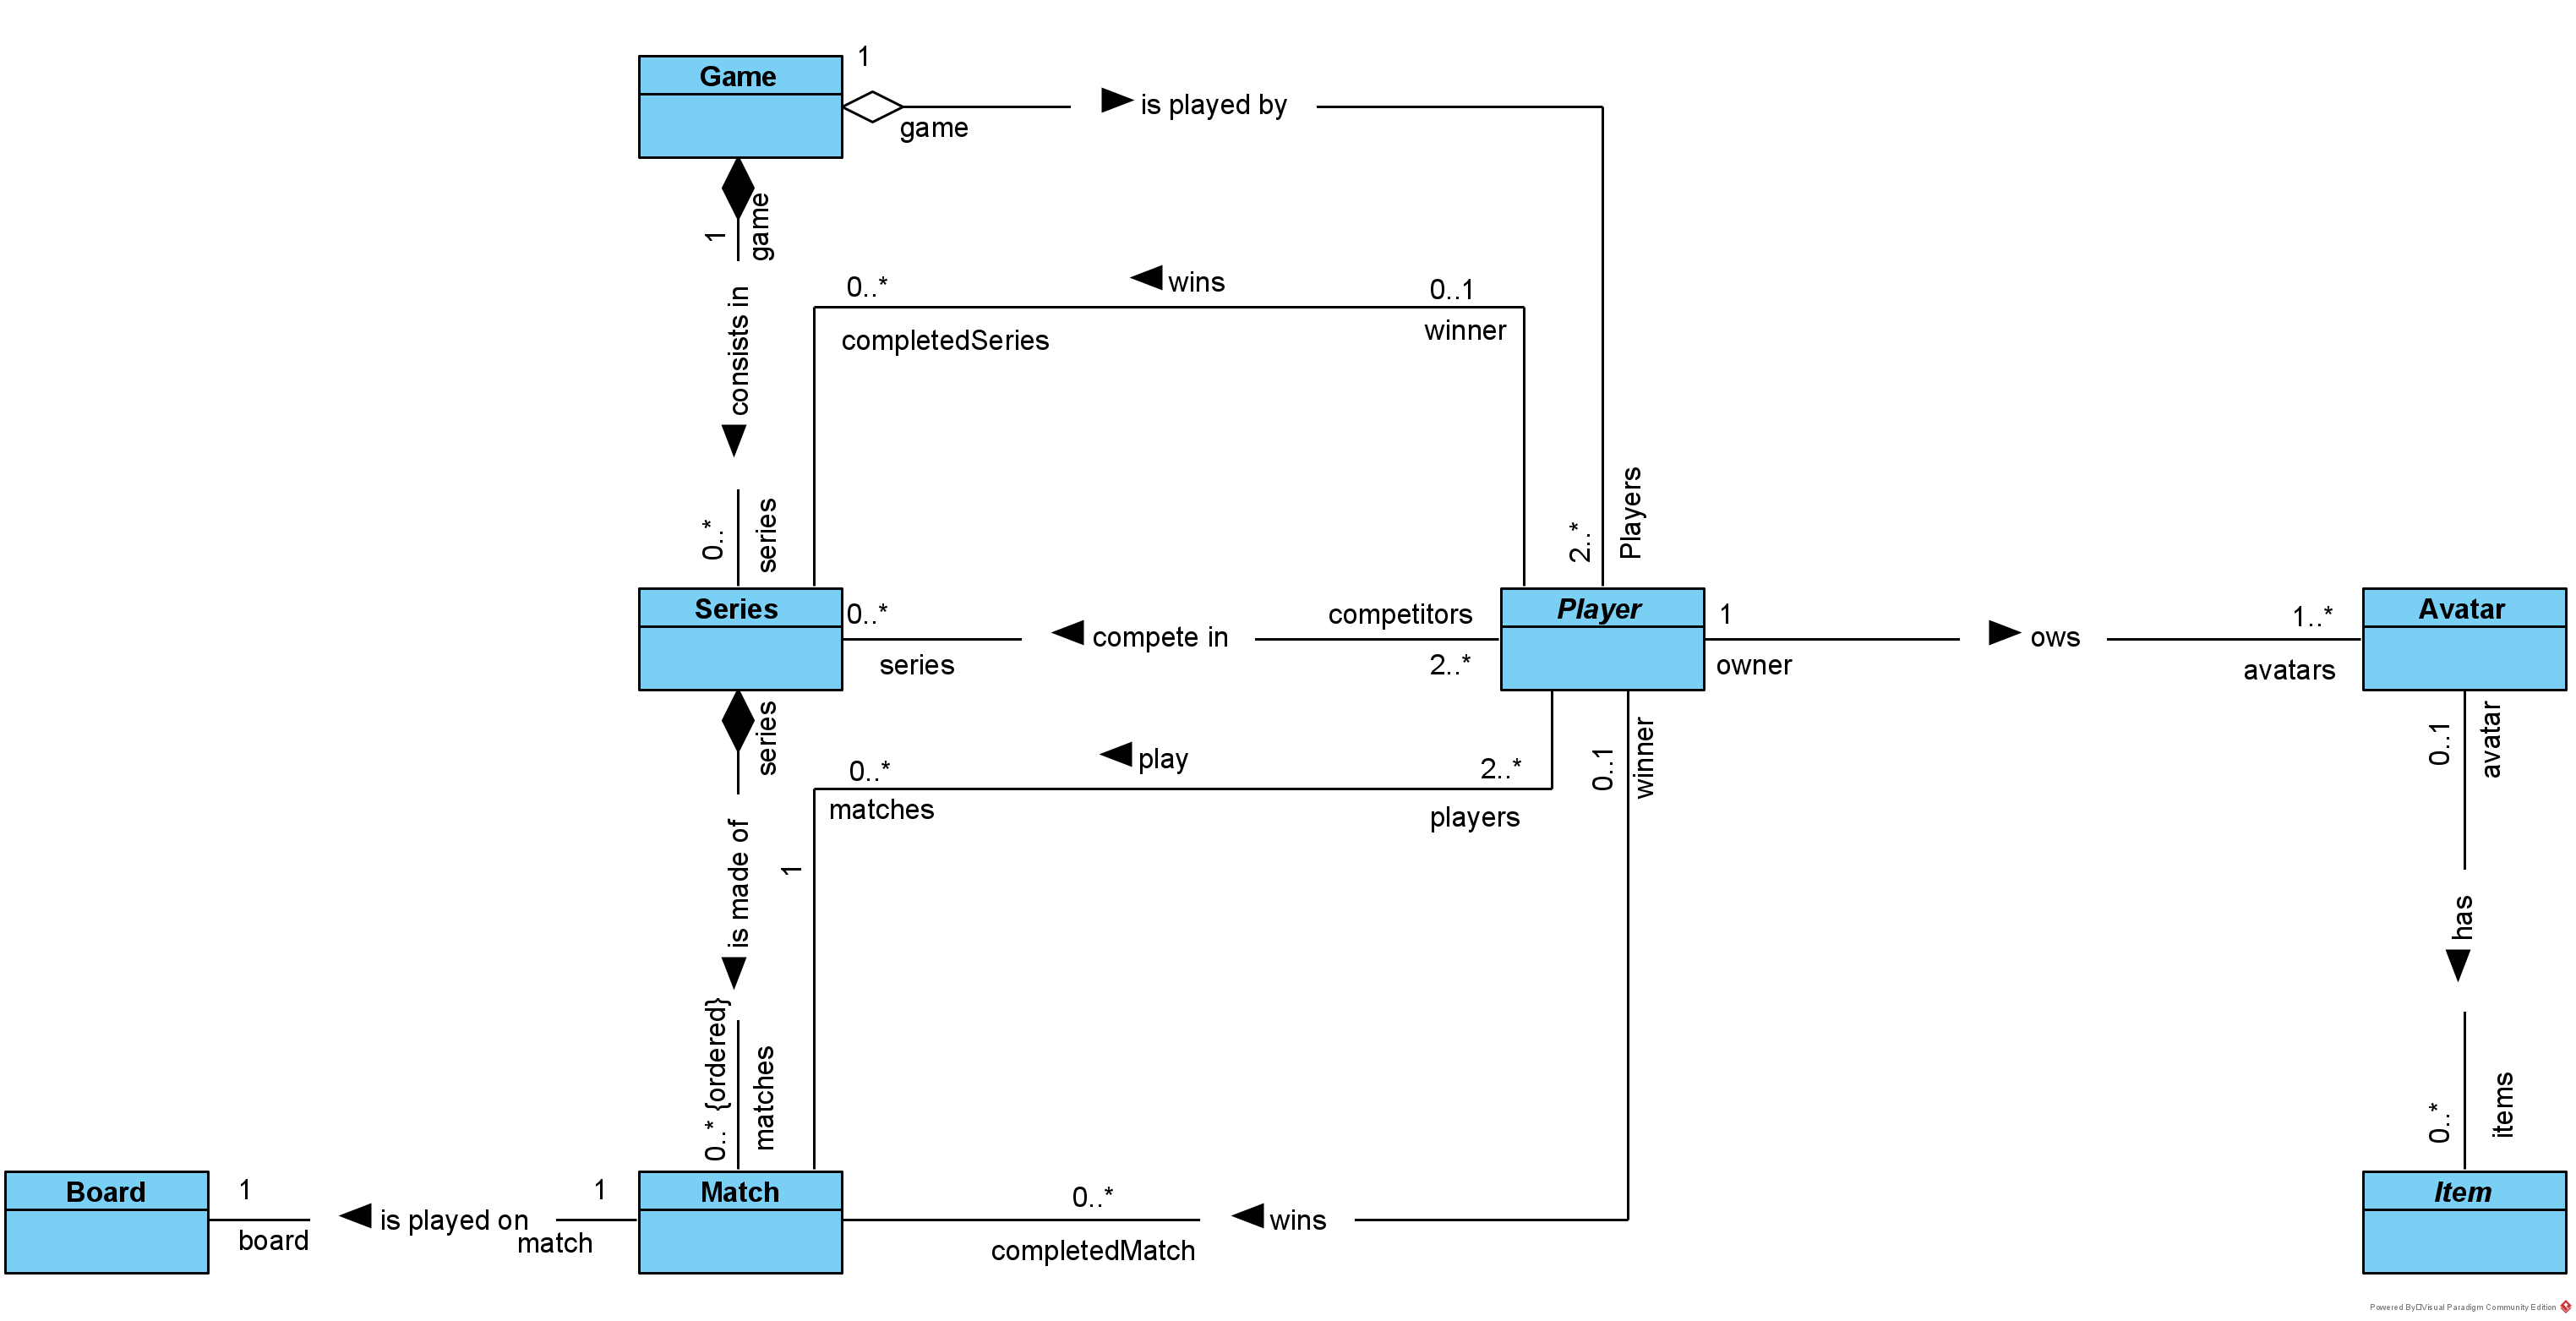
\includegraphics[width=\textwidth,height=.8\textwidth,keepaspectratio]{Diagrams/DJ-preversion.png}\newline
\end{center}

Le jeu décrit par les spécifications est un jeu d'exploration et de combat : des joueurs participent à des séries de rencontres. Sur le terrain d'une rencontre, les joueurs contrôlent des avatars : ils explorent un plateau de jeu, ramassent des objets et affrontent d'autres avatars ainsi que des monstres non-contrôlables. Pour gagner, les joueurs doivent soit tuer tous les autres joueurs (\textit{Battle Royale}) soit trouver la sortie en premier (\textit{Graal}).

\newpage
\section{Description détaillée}
\textbf{Question 4.2.}\label{Question 4.2.}

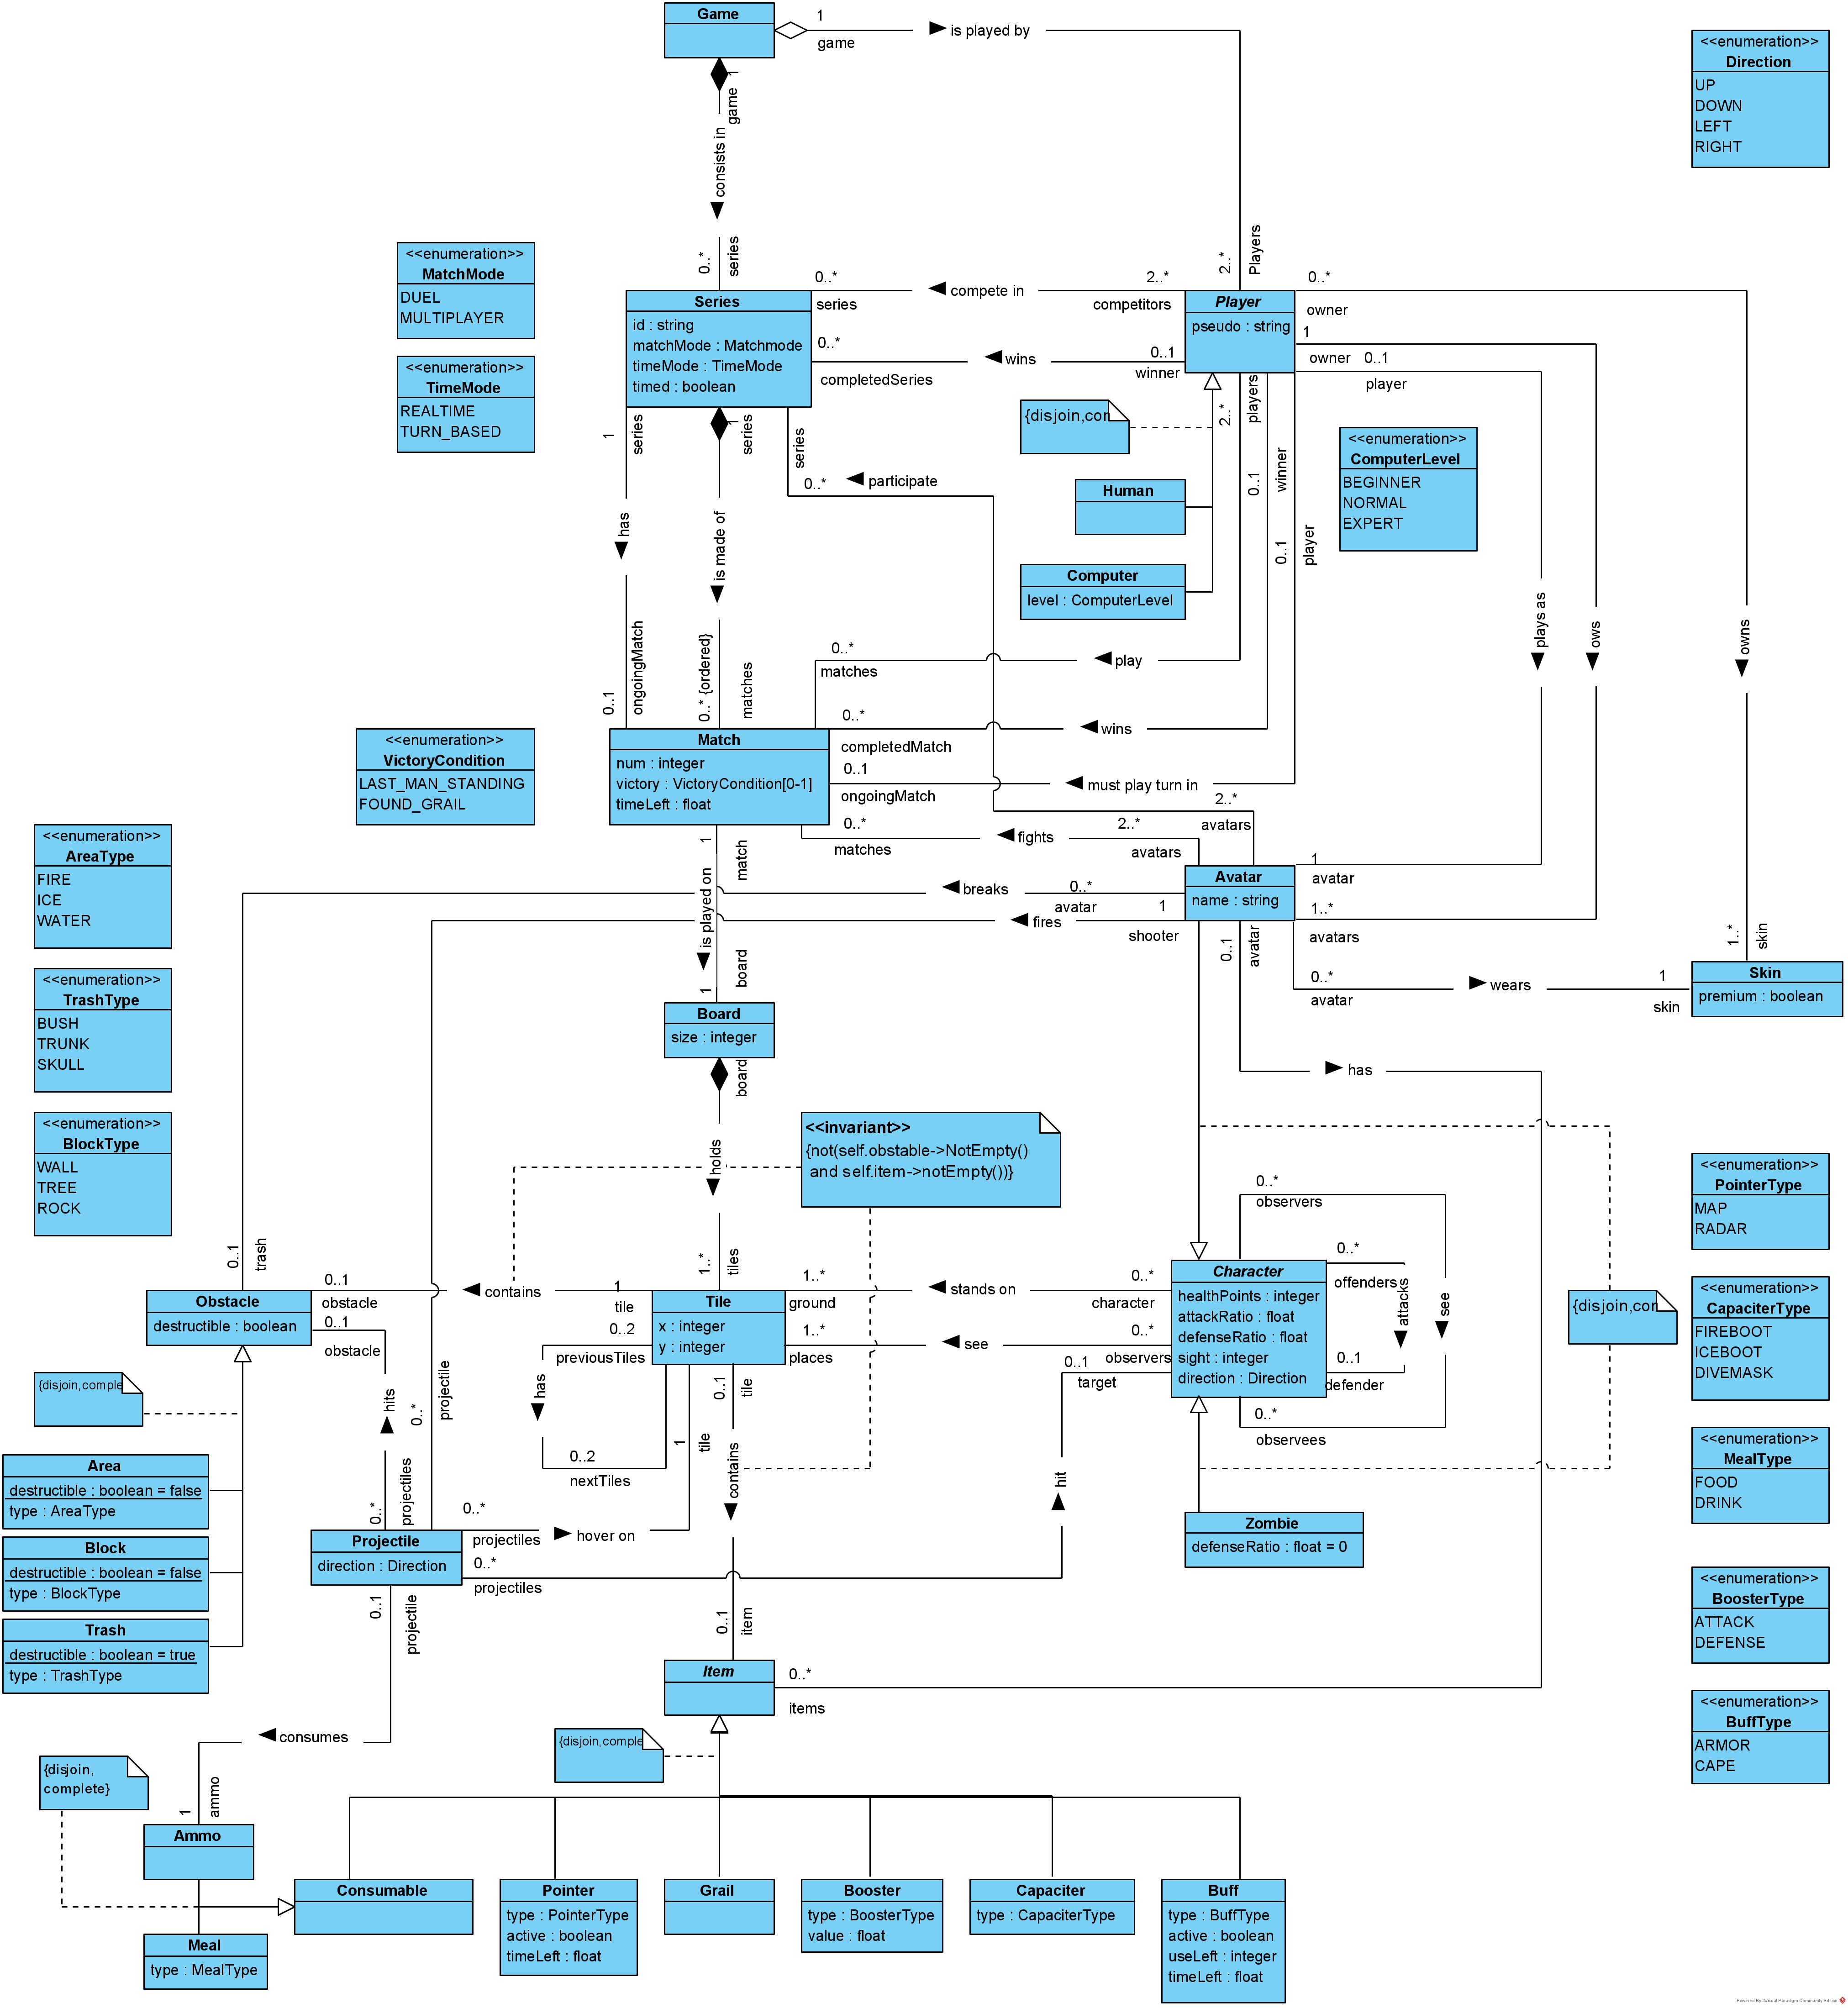
\includegraphics[width=\textwidth,height=\textheight,keepaspectratio]{Diagrams/DJ-fullversion.png}\newline

Dans cette section, nous détaillerons les diagrammes spécifiques aux différentes composantes de la définition du jeu, tel que donnée par les spécifications-client.

\subsection{Jeu}
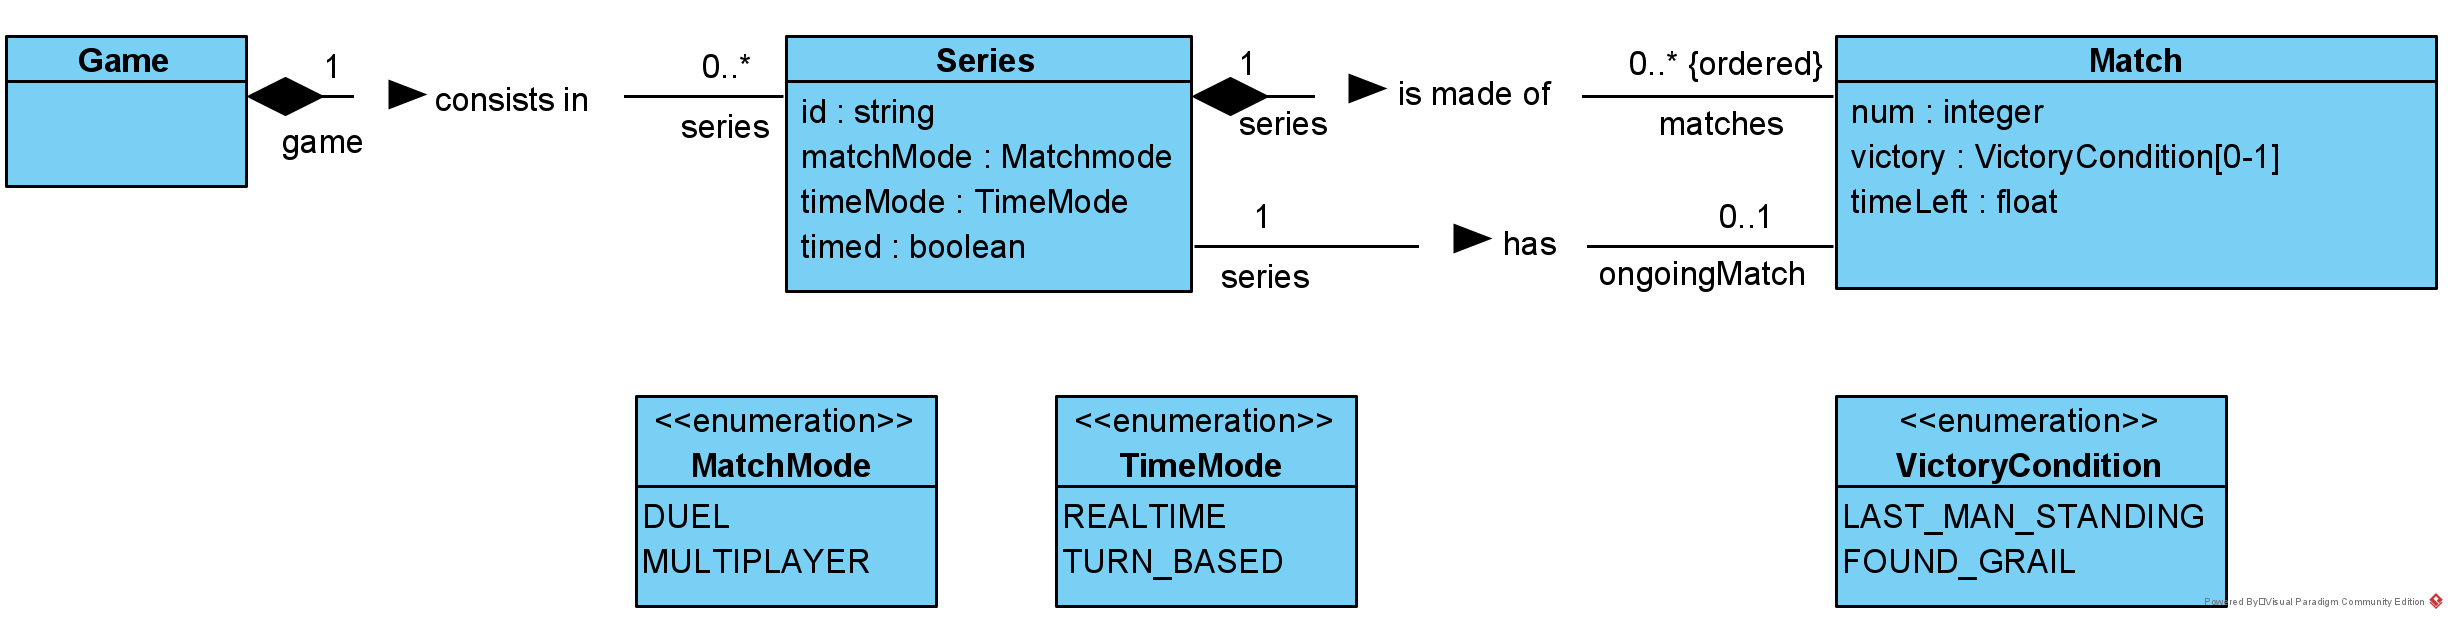
\includegraphics[width=\textwidth,height=\textheight,keepaspectratio]{Diagrams/DJ-Game.png}\newline

Le jeu décrit dans ce laboratoire est découpé en séries de rencontres : 
\begin{itemize}
    \item Le jeu est constitué d'un ensemble de séries.
    \item une série est composée d'au moins une rencontre.
\end{itemize}

Nous avons ainsi deux relations de \textit{composition} : 
\begin{itemize}
    \item Le jeu est composé de séries, c'est-à-dire que toute série implique nécessairement l'existence d'un jeu dont elle fait partie.
    \item La série est composée de rencontres et toute rencontre forme, de par son existence, au moins une série de 1 rencontre.
\end{itemize}

En termes de multiplicité, nous avons
\begin{itemize}
    \item pour un jeu, un ensemble non-ordonné de suites jouées.
    \item pour une série, un ensemble ordonné de rencontres, qui sont jouées de manière séquentielle.
    \item pour une série, il y a au maximum une rencontre en cours (soit il y a une rencontre en cours et la série continue, soit toutes les rencontres ont été jouées et la série est terminée).
\end{itemize}

Nous avons par ailleurs choisi de représenter les différents choix de mode et formule de jeux que peuvent poser les joueurs par des énumérations. En effet, il s'agit à chaque fois d'une information finie et restreinte, qu'il est facile d'énumérer. 

\begin{tcolorbox}
    Nous aurions pu utiliser des marqueurs booléens mais ceux-ci nous ont semblé moins porteurs d'information et d'expressivité dans le schéma. De plus, ils se seraient avérés moins flexibles si d'autres modes/formules devaient faire leur apparition par la suite.
\end{tcolorbox}

Enfin, un match comporte une condition de victoire : il ne s'agit ici pas d'une énonciation à l'instanciation de l'objet mais bien d'un marqueur signifiant (le cas échéant) qu'une rencontre a été remportée et de quelle manière.

\subsection{Joueur}

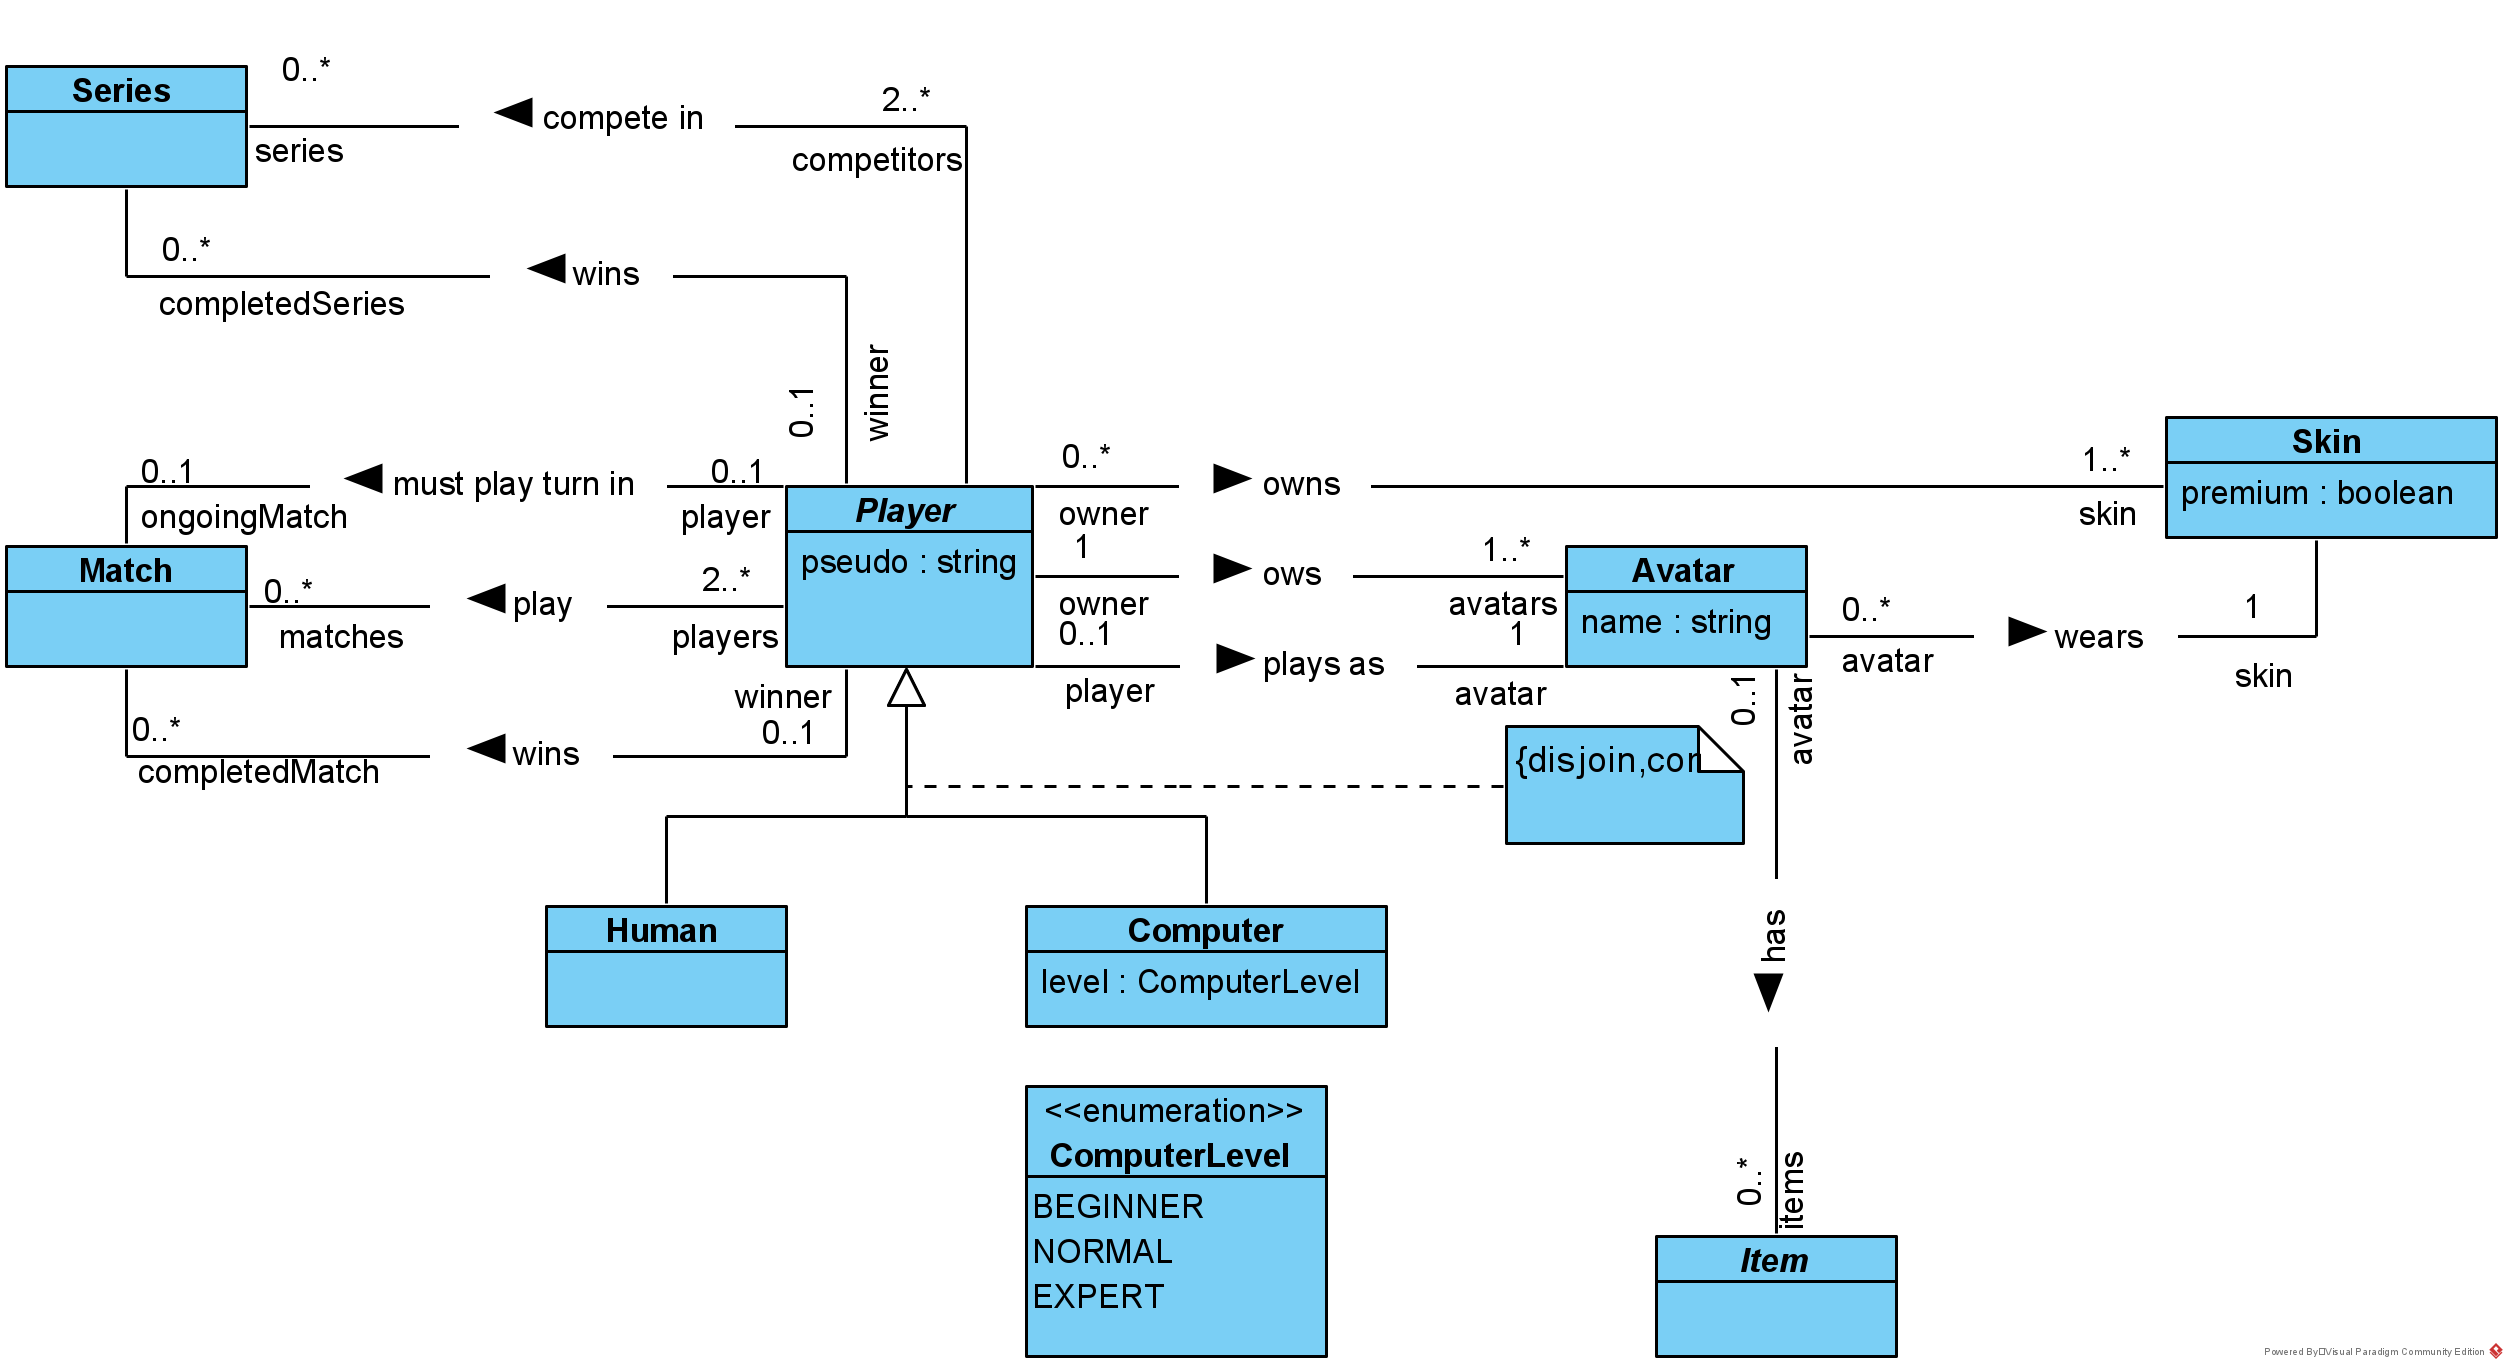
\includegraphics[width=\textwidth,height=\textheight,keepaspectratio]{Diagrams/DJ-Player.png}\newline

Le jeu est fait pour être joué : il a donc besoin de joueurs. 

Nous distingons ici deux sous-catégories de joueurs :
\begin{itemize}
    \item les joueurs humains et
    \item les joueurs-machine.
\end{itemize}

Nous avons ici spécifiquement une association de type \textit{spécialisation} : alors que les joueurs normaux (humains) ne possèdent qu'un nom, les joueurs-machine possèdent en plus un niveau de difficulté.
\begin{tcolorbox}
    En tant que telle, la classe \textit{Human} est redondante dans la relation de spécialisation. Nous aurions en effet pu nous contenter d'avoir une couverture incomplète pour distinguer les joueurs-machines des autres (qui sont les humains par déduction). Nous avons cependant choisi de garder cette classe sur notre diagramme pour des raisons d'expressivité.
\end{tcolorbox}

Un joueur est activement impliqué dans le jeu : il concourt dans des séries, qu'il peut gagner ou perdre, et il joue effectivement dans des rencontres, qu'il peut à nouveau gagner ou perdre. Lorsque le mode tour-par-tour est activé, le joueur peut en outre être appelé à jouer ou à attendre que son tour arrive. \newline

Chaque joueur est désigné par un pseudo qui lui est propre.
\begin{tcolorbox}
    Nous posons ici que même les joueurs-machine ont un pseudo (par ex. \textit{BOT\_1}).
\end{tcolorbox}

Les joueurs possèdent une galerie de personnages : des avatars utilisés dans le jeu et des apparences pour les personnaliser. \newline

En termes de multiplicité, nous avons posé les choix suivants :
\begin{itemize}
    \item Un joueur peut avoir joué un nombre indéfini de séries et de rencontre, allant de 0 pour les nouveaux arrivants à un nombre illimité pour les plus accros.
    \item Toute série et rencontre impliquent nécessairement au moins deux joueurs (aucun mode \textit{joueur vs environnement} n'est prévu). Il peut y en avoir davantage dans un mode multijoueur.
    \item Un joueur ne peut participer au maximum qu'à une rencontre et série à la fois.
    \item Il ne peut jamais y avoir plus qu'un gagnant par rencontre et par série.
        \begin{tcolorbox}
        La spécification du jeu précise que le gagnant d'une série est le joueur qui a remporté le plus de rencontres (raison pour laquelle celles-ci sont en nombre impair). Cette spécification ne tient pas compte du fait que des rencontres peuvent se terminer sans vainqueur parce que le chronomètre est écoulé. 
        Dans ce cas, puisque la spécification ne précise pas le comportement à adopter, le choix sera laissé au développeur de fixer une nouvelle règle : 
            \begin{itemize}
                \item personnage ayant trouvé le dernier Graal.
                \item personnage ayant tué le plus d'ennemis.
                \item ...
            \end{itemize}
        \end{tcolorbox}
    \item Un joueur dispose d'au moins un avatar, qui présente toujours une apparence (que le joueur a le loisir de changer).
    \item Un joueur possède au moins une apparence (par défaut) à appliquer à l'un de ses avatars.
\end{itemize}

\subsection{Plateau}
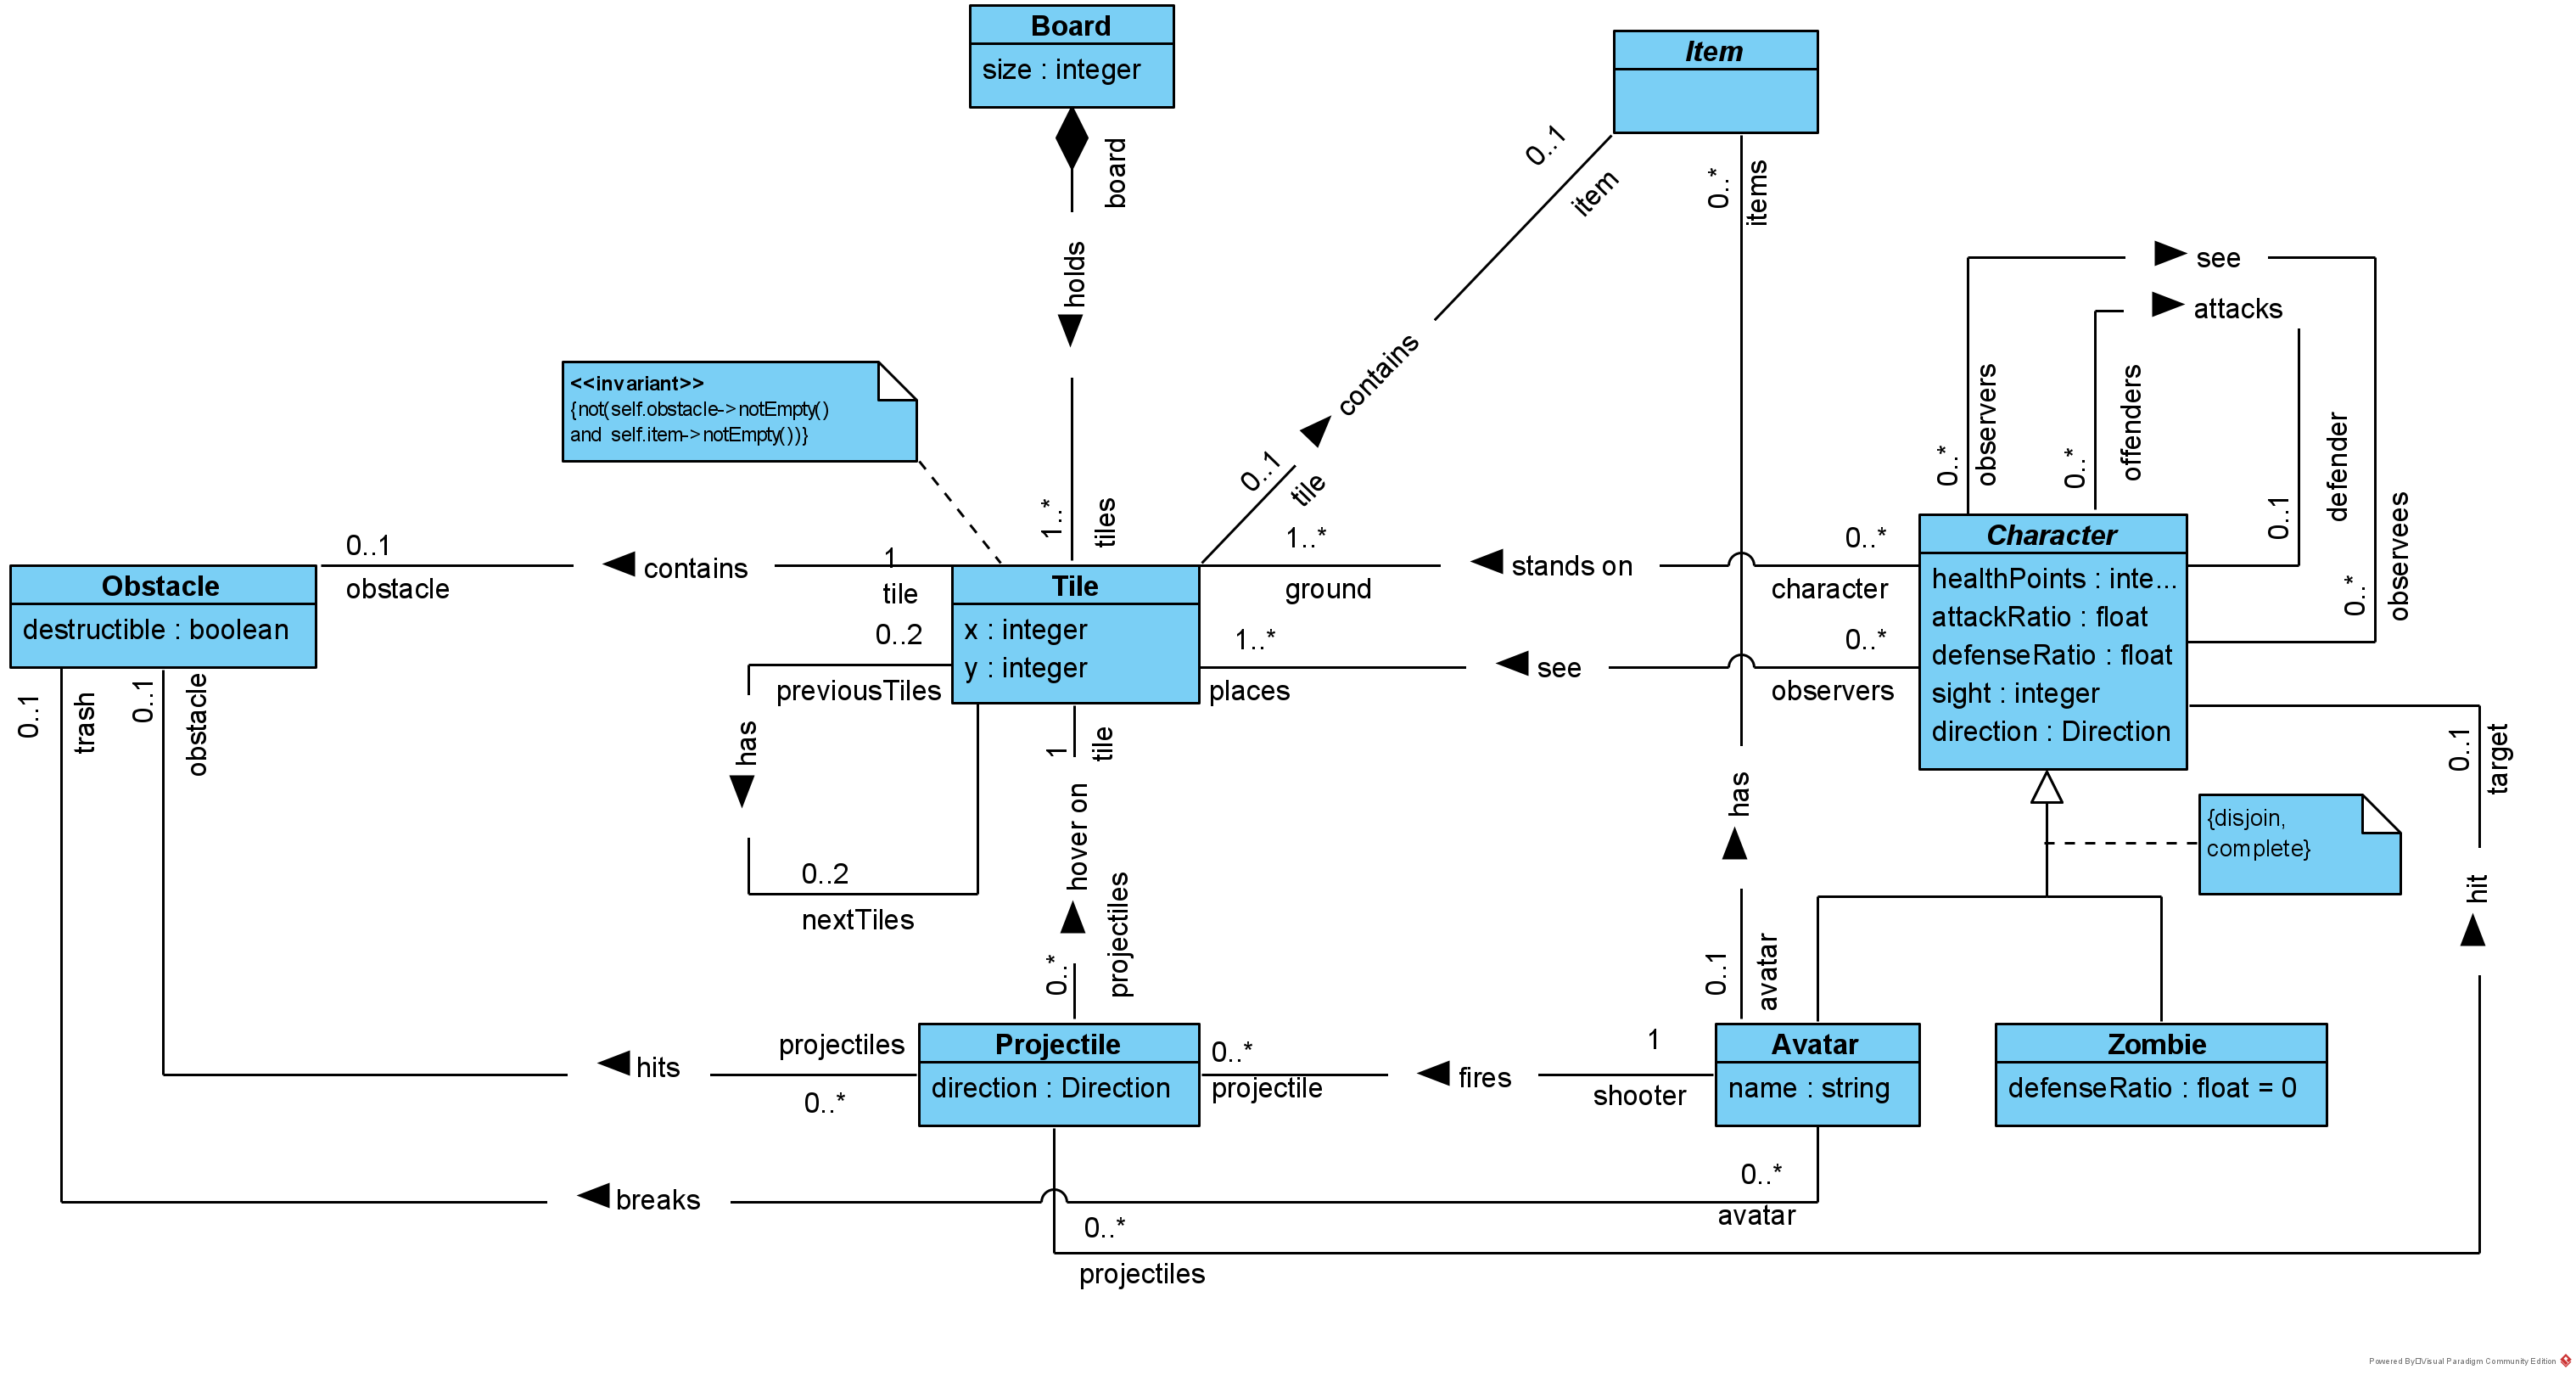
\includegraphics[width=\textwidth,height=\textheight,keepaspectratio]{Diagrams/DJ-Board.png}\newline

Le plateau est l'endroit-clé du jeu : c'est sur celui-ci que les joueurs passent la partie la plus importante du jeu, à explorer, ramasser et attaquer.\newline

Un plateau est constitué de tuiles : des cases numérotées et organisées de manière cardinale. Nous avons ici à nouveau une relation de \textit{composition}\,: un plateau est nécessairement composé de tuiles, et une tuile forme nécessairement au moins un plateau de 1 tuile. \newline

Sur ces tuiles déambulent des personnages : des entités animées, contrôlées par un joueur ou par l'ordinateur et pouvant se mouvoir sur le plateau. Ces personnages sont dotés de caractéristiques et de comportement uniformes : position, attaque et défense, champ de vision, mouvement, ...

En raison de cette uniformisation, nous avons choisi de déployer une super classe de \textit{généralisation} disjointe et complète : tout personnage est nécessairement soit un avatar, soit un zombie. \newline

Les avatars des joueurs sont dotés de capacités supplémentaires, par rapport aux zombies : ils peuvent ramasser des objets, tirer des projectiles ou encore tenter de casser des obstacles destructibles. Les objets qu'ils possèdent sont placés dans un inventaire.\newline
\begin{tcolorbox}
    Nous avons ici choisi de ne pas représenter conceptuellement l'inventaire sous forme de classe distincte, puisqu'il n'aurait pour seules associations que le fait de contenir des objets et appartenir à un avatar. Fonctionnellement, l'inventaire ne désigne que le regroupement des objets amassés par le joueur, ce qui est déjà signifié par l'association \textit{"{[}0..1{]} player has {[}0..*{]} items"} (un joueur peut amasser un nombre indéfini d'objets).
\end{tcolorbox}

En termes de multiplicité, nous avons posé les choix suivants :
\begin{itemize}
    \item Une tuile est située près d'autres tuiles de manière adjacente : 
        \begin{itemize}
            \item Deux tuiles situées à une position inférieure d'un facteur $x$ ou $y$.
            \item Deux tuiles situées à une position supérieure d'un facteur $x$ ou $y$.
        \end{itemize}
        \begin{center}
            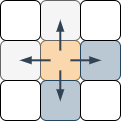
\includegraphics[height=2cm,keepaspectratio]{Images/Tile.png}    
        \end{center}
    \item Une tuile contient au maximum un obstacle ou un objet. La contrainte est ici exprimée en OCL car l'exclusion mutuelle n'est pas descriptible simplement sur le diagramme de classe.
    \begin{tcolorbox}
        Nous aurions pu gérer ce cas en rassemblant obstacles et objets sous une classe abstraite généralisant les objets \textit{statiques} (par opposition aux personnages dynamiques). Il aurait alors suffi de mettre une contrainte de cardinalité [0..1] pour ne permettre la présence que d'un objet ou d'un obstacle sur une tuile. Nous avons choisi de ne pas le faire car nous estimions qu'ils restaient conceptuellement fort éloignés.
    \end{tcolorbox}
    \item Une tuile n'est suffisante que pour accommoder au maximum un personnage, qu'il s'agisse d'un zombie ou d'un avatar.
    \item Un avatar peut ramasser un objet ou tirer un projectile. De manière inverse, tout objet doit être ramassé/tout projectile doit nécessairement être lancé par un avatar.
    \item Un personnage peut voir autant de personnages que le permet son champ de vision. De même, ce personnage peut être vu par autant de personnages que leur champ de vision le leur permet. Il ne s'agit ici pas d'une relation réflexive : un personnage qui en voit un autre n'est pas forcément aperçu par cet autre personnage, car ils ne partagent pas le même champ de vision.
    \item Un personnage ne peut jamais attaquer plus d'un seul personnage (situé en face de lui). Il peut en revanche être attaqué par plusieurs personnages/touché par plusieurs projectiles à la fois (s'il est encerclé).
\end{itemize}

\subsection{Obstacle}
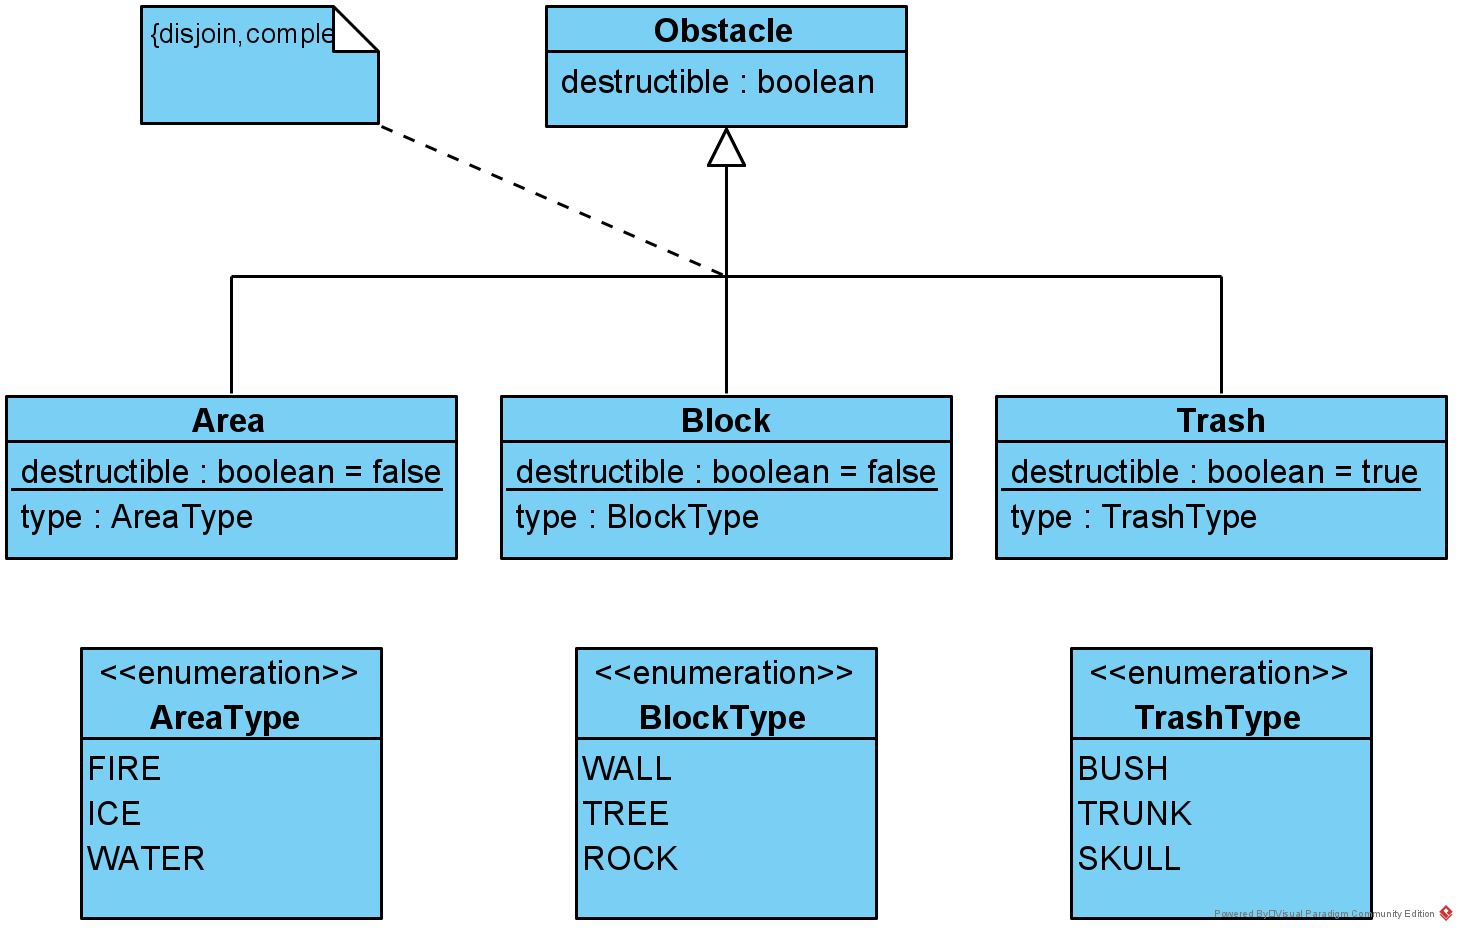
\includegraphics[width=\textwidth,height=\textheight,keepaspectratio]{Diagrams/DJ-Obstacle.png}\newline

Les obstacles sont des éléments fixes du décor, qui peuvent empêcher ou gêner le personnage. \newline

De par les spécifications, nous savons que tout obstacle est traversable par le truchement d'objets. Dès lors, notre catégorisation repose davantage sur des caractéristiques plus pérennes entre les objets :
\begin{itemize}
    \item Certains obstacles sont destructibles (les crasses).
    \item Certains obstacles sont permanents et inactifs (les blocs).
    \item Certains obstacles sont permanents et offrent un certain niveau d'interaction (les zones).
\end{itemize}
Ces obstacles sont mutuellement exclusifs, nous avons donc choisi une relation de \textit{spécialisation} disjointe et complète.
\begin{tcolorbox}
    Nous avons également choisi de marquer la capacité de \textit{destructibilité} par un booléen défini au niveau des classes et non des instances, puisqu'il s'agit d'un trait spécifique à chaque classe mais immuable.
\end{tcolorbox}

\subsection{Objet}
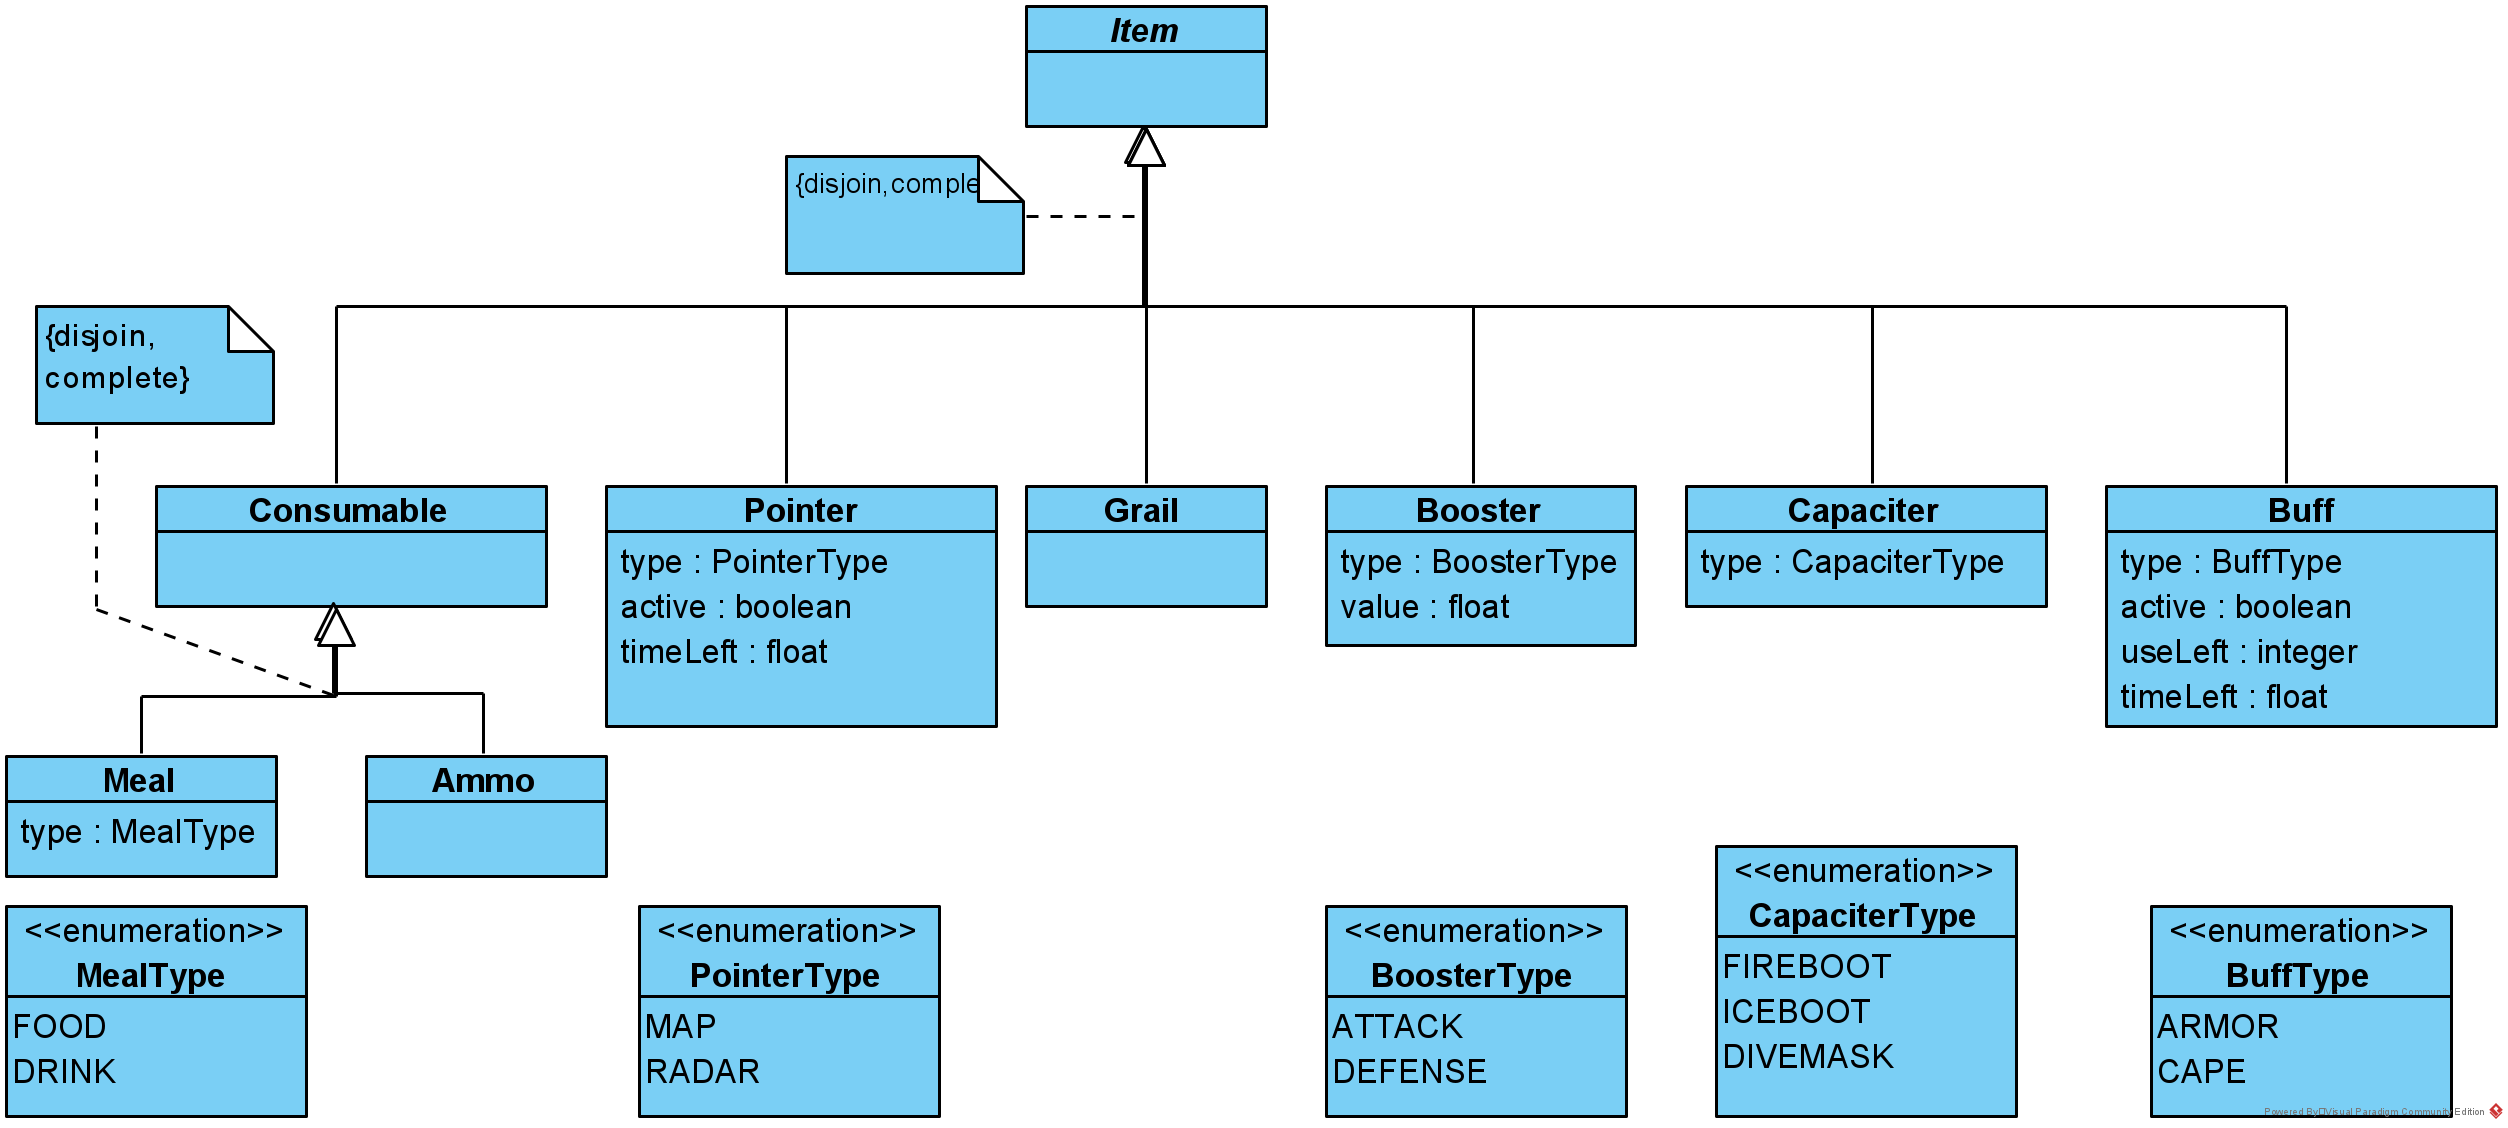
\includegraphics[width=\textwidth,height=\textheight,keepaspectratio]{Diagrams/DJ-Item.png}\newline

Les objets sont des éléments fixes du décor dont le joueur va pouvoir s'emparer pour s'aider dans sa quête.\newline

Comme pour les obstacles, nous avons choisi de dissocier les objets en fonction de leur comportement.
\begin{itemize}
    \item Les consommables (\textit{Consumable}) sont des objets \textit{jetables} dont la fonction est d'être accumulé puis utilisé par l'avatar. 
    \item Les pointeurs (\textit{Pointer}) sont des objets aidant à l'orientation et non accumulables (seule une unique version est conservée, dont on manipule ensuite le compteur).
    \item Le Graal (\textit{Grail}) est le graal, simplement.
    \item Les améliorants (\textit{Booster}) sont des objets instantanés, qui augmentent immédiatement le potentiel de l'avatar.
    \item Les capaciteurs (\textit{Capaciter}) sont des objets permanents conférant au personnage des nouvelles capacités.
    \item Les super-pouvoirs (\textit{Buff}) sont des objets puissants, trouvables en faible quantité et conférant à leur porteur un avantage critique. Ils sont caractérisés par une durée limitée d'utilisation.
\end{itemize}

Il s'agira ici plus d'une association de \textit{spécialisation}, mettant en avant les caractéristiques susmentionnées. Nous avons en outre inclus une sous-spécialisation des consommables, pour signifier l'effet : gain de vie versus munition pour lancer de projectiles.\newline

Pour des raisons d'expressivité et parce que la liste des valeurs possibles est définie et limitée, nous avons choisi d'utiliser des énumérations pour représenter les types finaux possibles des objets.\newline

Il existe par ailleurs deux catégories d'objets qui disposent d'un temps d'utilisation limité : les pointeurs et les super-pouvoirs. Pour représenter l'écoulement du temps, nous avons choisi d'utiliser un seul compteur (\textit{timeLeft}) dont nous faisons varier l'unité en fonction du mode de jeu choisi :
\begin{itemize}
    \item S'il s'agit d'une rencontre en mode tour-par-tour, le compteur sera décrémenté à chaque fin de tour (via des valeurs entières).
    \item S'il s'agit d'une rencontre en mode temps-réel, le compteur sera décrémenté au fur et à mesure du temps qui passe (via des valeurs décimales).
\end{itemize}

\section{Contraintes d'unicité}
\textbf{Question 4.3.}\label{Question 4.3.}
\begin{itemize}
    \item \textit{les matchs sont identifiés de manière unique au sein du jeu ;}
        \begin{lstlisting}
context Game inv uniqueSeries : 
    self.series->forAll(s1,s2|s1<>s2 implies s1.id<>s2.id)
        \end{lstlisting}
        Pour tout jeu donné, toute série différente possède nécessairement un identifiant différent.
        
    \item \textit{les joueurs ont des pseudos différents au sein du jeu ;}
        \begin{lstlisting}
context Game inv uniquePlayer : 
    self.players->forAll(p1,p2|p1<>p2 implies p1.pseudo<>p2.pseudo)
        \end{lstlisting}
    Pour tout joueur donné, s'il existe un autre joueur distinct alors celui-ci aura un pseudo différent.
    
    \item \textit{les personnages/avatars d'un joueur sont nommés différemment, et ont une représentation physique distincte pour pouvoir les reconnaître visuellement au premier coup d'oeil ;}
        \begin{lstlisting}
context Player inv distinctAvatars : 
    self.avatars->forAll(a1,a2|(a1.id=a2.id or a1.skin=a2.skin) implies a1=a2)
        \end{lstlisting}
        Pour tout joueur donné, un même nom ou une même apparence ne peut appartenir qu'à un seul avatar.

    \item \textit{les rencontres d'un match portent un numéro d'ordre unique ;}
        \begin{lstlisting}
context Series inv distinctMatchNum : 
    self.matches->forAll(m1,m2|m1<>m2 implies m1.num <>m2.num)
        \end{lstlisting}
        Pour toute série donnée, l'ensemble des rencontres qui la composent possèdent un numéro différent entre elles.
\end{itemize}

\section{Contraintes de règles}
\textbf{Question 4.4.}\label{Question 4.4.}
\begin{itemize}
    \item \textit{le potentiel de vie d'un joueur est toujours positif ;}
        \begin{lstlisting}
context Character inv positiveHealth : 
    self.healthPoints > 0
        \end{lstlisting}
    Pour un personnage donné, sa santé est toujours positive (sinon, il est mort et enterré \textdagger).
    
    \item \textit{les ratios d'attaque et de défense sont des ratios, c'est-à-dire des valeurs strictement positives et inférieures à 1 ;}
        \begin{lstlisting}
context Character inv positiveAR : 
    self.attackRatio > 0 and self.attackRatio < 1
        \end{lstlisting}
        \begin{lstlisting}
context Avatar inv positiveDR : 
    self.defenseRatio > 0 and self.defenseRatio < 1  
        \end{lstlisting}      
        \begin{lstlisting}
context Zombie inv zeroDR : 
    self.defenseRatio = 0
        \end{lstlisting}
    
    Pour tout personnage donné, le ratio d'attaque est systématiquement compris entre 0 et 1 exclus. Par contre, seuls les avatars ont un ratio de défense non-nul (puisqu'il est spécifié que les zombies n'ont pas de défense).
    
    \item \textit{le nombre de rencontres constituant un match est toujours impair ;}
        \begin{lstlisting}
context Series inv oddNumberOfmatches : 
    self.matches->size().mod(2)=1
        \end{lstlisting}
    Pour toute série, le reste de la division par deux doit être 1 (ce qui signifie qu'il est impair).

    \item \textit{le numéro identifiant la rencontre au sein d'un match correspond à l'ordre dans lequel il sera joué (ou plus précisément, l'ordre dans la collection qui le stocke, à supposer que les rencontres sont jouées dans l'ordre de stockage) ;}
        \begin{lstlisting}
context Series inv matchNumEqualsOrder : 
    self.matches->forAll(m|self.matches->at(m.num)=m)
        \end{lstlisting}
    Pour toute série, on trouve à chaque indice un match dont le numéro est égal à cet indice.

    \item \textit{l'inventaire d'un joueur contient trois types d'items : les items ramassables (nourriture, boisson ou munitions), les objets d'aide à l'orientation, et les objets d'aide (cotte de maille et cape) ;}
        \begin{lstlisting}
context Avatar inv inventory : 
    self.items->forAll(i|i.oclIsKindOf(Item) and 
                         not(i.oclIsTypeOf(Grail))and
                         not(i.oclIsTypeOf(Booster)))
        \end{lstlisting}
    Pour un avatar donné, tous les éléments de l'inventaire sont des objets de super type \textit{Item}, mais aucun n'est le Graal ni un booster (qui sont consommés immédiatement).
    
    \item \textit{une seule des cases d'un monde contient un Graal ;}
        \begin{lstlisting}
context Board inv onlyOneGrail : 
    self.tiles.item->one(oclIsTypeOf(Grail))
        \end{lstlisting}
        Pour un plateau donné, de tous les objets présents sur toutes les tuiles, seul un est le Graal.

    \item \textit{les coordonnées d'une case ne peuvent excéder la longueur d'un monde ;}
        \begin{lstlisting}
context Board inv tileNotExceedLimit : 
    self.tiles->select(t|t.x<1 or 
                         t.x>self.size or 
                         t.y<1 O 
                         t.y>self.size)->isEmpty()
        \end{lstlisting}
    Pour un plateau donné, il n'existe aucune tuile dont l'un des paramètres est hors-limite (en dehors de l'intervalle \textit{{[}1:size{]}}).
    
    \item \textit{la disposition des cases correspond à leur coordonnées. Par exemple, l'abscisse d'une case à droite d'une case donnée est l'entier successeur de l'abscisse de la case de référence (et similairement pour les autres directions, en tenant compte des bords du plateau) ;}
        \begin{lstlisting}
context Board inv isFull : 
    self.tiles.count()=(self.size * self.size)
        \end{lstlisting}
        \begin{lstlisting}
context Board inv noDuplicateTile : 
    self.tiles->forAll(t1,t2|(t1.x=t2.x and t1.y=t2.y)
                             implies t1=t2)
        \end{lstlisting}
\begin{minipage}{\linewidth}
        \begin{lstlisting}
context Board inv isNextTo : 
    self.tiles->forAll(t1,t2|t1.nextTiles->includes(t2) 
                             implies (t2.x=t1.x+1 and t2.y=t1.y  ) or
                                     (t2.x=t1.x   and t2.y=t1.y+1))
        \end{lstlisting}
\end{minipage}
        \begin{lstlisting}
context Board inv onlyOneFirstTile : 
    self->previousTiles->isEmpty() implies self.x=1 and self.y=1
        \end{lstlisting}
    Pour un plateau donné, pour chacune des cases, une case qui est voisine suivante d'une autre a nécessairement soit un x plus grand de 1, soit un y plus grand de 1.
    \begin{itemize}
        \item Une tuile peut avoir deux voisines: 1 au sud, 1 à l'est, par exemple pour la case $1\,\times\,1$.
        \item Une tuile peut avoir seulement une voisine (si elle se trouve en extrémité de plateau par un côté)
        \item Une tuile peut avoir zéro voisine (si elle se trouve en tout fin du plateau, à $size \times size$).
        \item La seule tuile qui n'a aucune tuile précédente est la tuile $1\times 1$.
    \end{itemize}

    \begin{tcolorbox}
        Si on combine les règles \textit{isNexto}, \textit{tileNotExceedLimit}, \textit{isFull} et \textit{onlyOneFirstTile}, on obtient par récurrence que les tuiles sont placées au bon emplacement et que le plateau n'a pas de case manquante : il existe le bon nombre de tuiles, qui sont toutes différentes et comprises dans les limites du plateau, qui sont placées par ordre croissant et dont la première est nécessairement la tuile $1\,\times\,1$.   
    \end{tcolorbox}
    
    \item \textit{un joueur se trouve toujours dans la case correspondant à sa position absolue ;}

    Pas de contrainte OCL à exprimer ici.
    \begin{tcolorbox}
        Un personnage est lié au maximum à une et une seule case :
        \begin{itemize}
            \item soit il est utilisé par le joueur dans une partie définie et alors, sa position absolue est fonction de la case (\textit{ground}) sur laquelle il se trouve.
            \item soit il n'est pas utilisé par le joueur, n'est donc pas présent sur le plateau et n'a dès lors pas de position absolue.
        \end{itemize}
    Dès lors que le personnage n'est lié qu'à une seule case, il est possible d'en déduire sa position absolue depuis cette case.
    \end{tcolorbox}
    
    \item \textit{la bordure d'un plateau contient toujours des éléments infranchissables (pour éviter aux personnages de « sortir » du monde) ;}
        \begin{lstlisting}
context Board inv isWalled : 
    self.tiles.forAll(t|(t.x=1 or
                         t.x=self.size or
                         t.y=1 or
                         t.y=self.size)
        implies t.obstacle.oclIsKindOf(Block))
        \end{lstlisting}
        Pour toute tuile du jeu, si celle-ci est comprise à une extrémité (càd qu'un des paramètres de sa position est 1 ou la taille), alors elle doit contenir un obstacle de sous-type de \textbf{Block}.
        
        \begin{tcolorbox}
            Cette règle n'empêchera pas un joueur qui possède une cape de mage de sortir de la cape, puisque celle-ci lui permet de traverser tout obstacle, même ceux de type \textit{Block}. \newline
            Pour empêcher un joueur de sortir effectivement, il faudra utiliser les coordonnées de la case de destination pour vérifier que le mouvement est valide.
        \end{tcolorbox}
    
    \item \textit{Le nombre de cases visibles correspond à la valeur de visibilité liée au joueur. Par exemple, dans le plateau à droite dans la Figure 2, la visibilité de 3 rend « découvertes » trois lignes au-dessus, en dessous, et trois colonnes à droite et à gauche ;} 
        \begin{lstlisting}
context Avatar inv canSeeTile : 
    self.visibleTiles->forAll(t|t.x <= self.ground.x+self.sight and
                                t.x >= self.ground.x-self.sight and
                                t.y <= self.ground.y+self.sight and
                                t.y >= self.ground.y-self.sight)
        \end{lstlisting}
        Pour un personnage donné, les tuiles visibles sont celles dont la position est incluse dans deux intervalles au centre desquels se trouve le personnage:
        \begin{itemize}
            \item {[}x-sight: x+sight{]}
            \item {[}y-sight: y+sight{]}
        \end{itemize}
    
    \item \textit{un personnage ne peut pas se trouver sur une case portant un obstacle infranchissable ;}
    \begin{samepage}
        \begin{lstlisting}
context Tile inv nonCrossableObstacle : 
    self.obstacle->notEmpty() and self.character->notEmpty()
    implies 
         self.character.oclIsTypeOf(Avatar) and
        (self.obstacle.oclIsTypeOf(Area) and
                (self.obstacle.type=AreaType::FIRE 
            or  (self.obstacle.type=AreaType::ICE and
                 self.character->oclAsType(Avatar).items
                    ->select(i|i.oclIsTypeOf(Capaciter) and
                               i.type=CapaciterType::ICEBOOT)->notEmpty()) 
            or  (self.obstacle.type=AreaType::WATER and
                 self.character->oclAsType(Avatar).items
                    ->select(i|i.oclIsTypeOf(Capaciter) and
                               i.type=CapaciterType::DIVEMASK)->notEmpty())))
    or (self.obstacle.oclIsTypeOf(Area) and
        self.character->oclAsType(Avatar).items
            ->select(i|i.oclIsTypeOf(Buff) and
                       i.type=BuffType::CAPE)->notEmpty())
    or (self.character.items
            ->select(i|i.oclIsTypeOf(Buff) and
                       i.type=BuffType::CAPE and
                       i.useLeft>0)->notEmpty()))
        \end{lstlisting}
    \end{samepage}
    \begin{samepage}
    Si, sur une tuile donnée, on trouve un avatar et un obstacle, alors cela implique que
    \begin{itemize}
        \item soit l'obstacle est une zone de feu (et le joueur peut le franchir au prix de points de vie),
        \item soit l'obstacle est une zone de glace et le personnage possède un capaciteur "botte à crampons" dans son inventaire,
        \item soit l'obstacle est une zone d'eau et le personnage possède un capaciteur "kit de plongée" dans son inventaire,
        \item soit l'obstacle est un obstacle de zone et le personnage possède la cape de mage,
        \item soit l'obstacle est n'importe quel autre obstacle et le personnage possède la cape de mage avec des points d'utilisation restants.
    \end{itemize}
    \end{samepage}

\begin{tcolorbox}
    Nous acceptons ici plusieurs postulats :
    \begin{itemize}
        \item Les obstacles destructibles sont infranchissables tant qu'ils ne sont pas détruits (sauf avec la cape), et disparaissent quand ils sont détruits.
        \item La cape reste suffisante pour pouvoir traverser les zones \textit{feu-eau-glace}, même si elle n'a plus de point d'utilisation restant: on pourrait ainsi imaginer une situation où le joueur conserve la cape après expiration de son utilisation pour les obstacles infranchissables.
        \item La cape qui n'a plus de temps (tour) actif restant est retirée de l'inventaire et ne doit donc pas être testée pour son(ses) temps (tours) restant(s).
    \end{itemize}
\end{tcolorbox}
    
    \item \textit{deux personnages (y compris les zombies) ne peuvent pas se trouver sur la même case ;}
    
    
    Il n'est pas nécessaire de vérifier par OCL si deux personnages sont sur une même tuile car cela est déjà réglé par la cardinalité de la relation \textit{"{[}0..1{]} character stands on {[}0..1{]} ground"}.
    
    Nous avons ici deux aspects :
    \begin{itemize}
        \item Un personnage ne se trouve pas nécessairement sur une tuile : cette cardinalité est rendue nécessaire par le fait qu'un joueur peut posséder un avatar sans jouer à une partie. Dès lors qu'il n'est pas en partie, il ne peut y avoir de tuile sur laquelle se trouver. Il faut donc admettre le cas où il n'existe pas de tuile pour un avatar donné.
        
        Les zombies doivent en revanche nécessairement avoir une tuile, puisqu'ils n'existent que pour un monde à la fois. Cette contrainte doit être exprimée en OCL.
        \begin{lstlisting}
context Zombie inv alwaysOnTile:
    self.ground->notEmpty()
        \end{lstlisting}
        \item Une tuile ne comprend pas nécessairement un personnage : toutes les tuiles ne sont en effet pas occupées (sinon, le plateau serait rempli de joueurs... et le jeu serait injouable).
    \end{itemize}
    
\end{itemize}

\begin{minipage}{\textwidth}
\section{Question de stratégies}

\textbf{Question 4.5.}\label{Question 4.5.}\newline

\textit{La définition des deux DSLs, pour spécifier les mondes et pour définir les stratégies, est séparée en deux morceaux. Cependant, pour que le jeu soit utilisable, ces deux éléments doivent être harmonieusement connectés. Comment, et où, apparaît la notion de stratégie dans votre Diagramme de Classes pour spécifier les mondes?}\newline

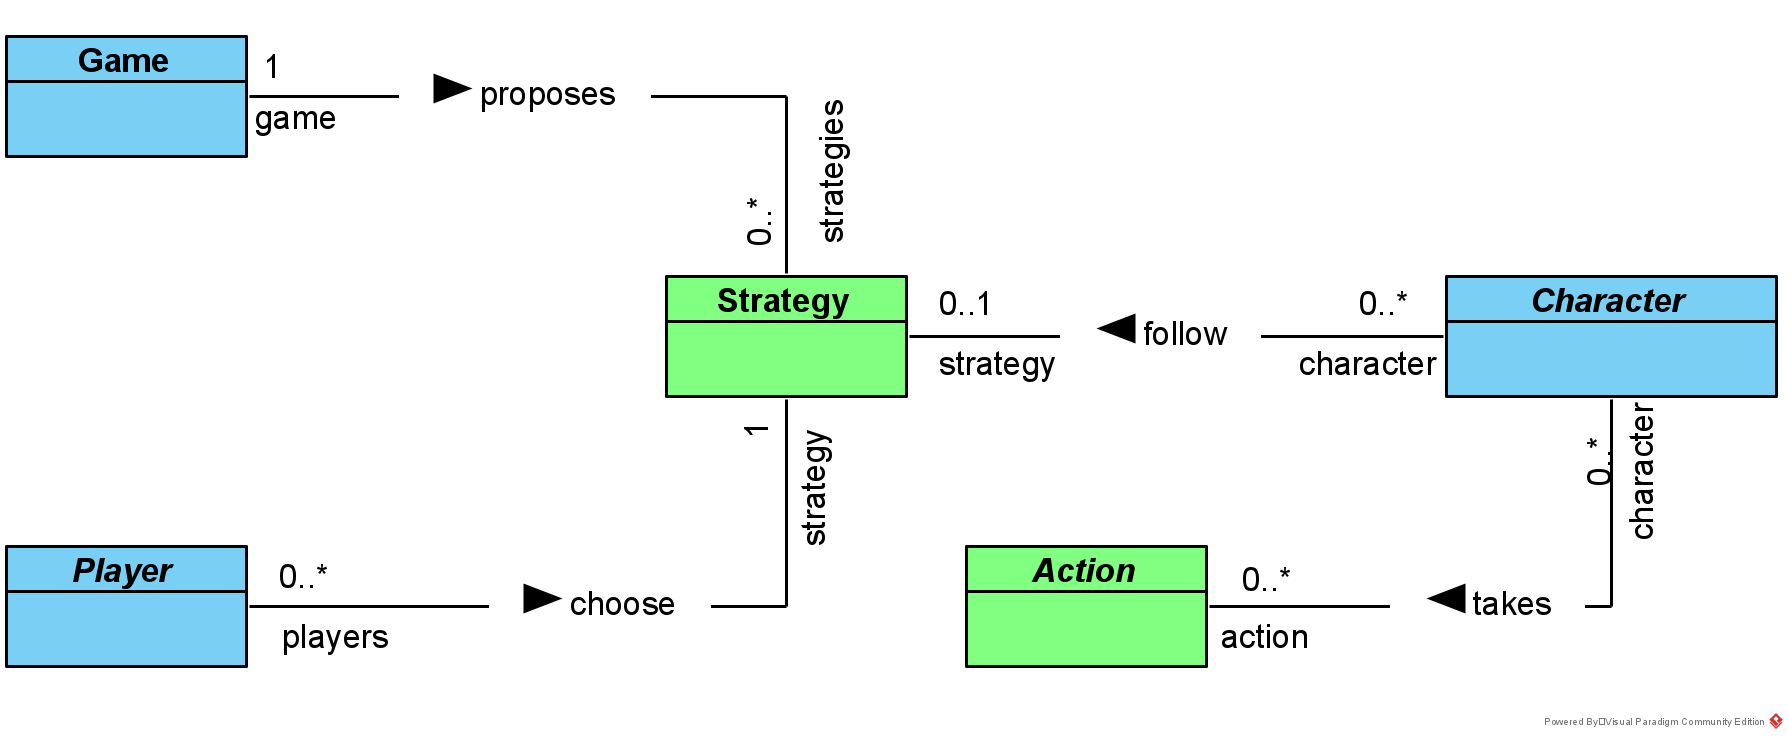
\includegraphics[width=\textwidth,height=\textheight,keepaspectratio]{Diagrams/DJ-Strategy.png}
\end{minipage}
\begin{samepage}
La notion de stratégie doit apparaître à quatre endroits :
\begin{itemize}
    \item Dans la définition même du jeu, au sein d'une liste ayant été élaborée par les développeurs pour permettre de jouer en mode tour-par-tour.
    \item Dans le choix que peuvent faire les joueurs de la stratégie à suivre au cours d'une rencontre tour-par-tour.
    \item Dans le comportement des personnages, qui suivent une stratégie dans une rencontre tour-par-tour: les avatars qui suivent la stratégie choisie par leur propriétaire et les zombies qui appliquent une stratégie par défaut, que l'on suppose être long-terme=RANDOM, court-terme=ATTACK (les zombies errent sans but jusqu'à apercevoir un avatar qu'ils vont tenter d'occire prestement).
    \item Dans les actions concrètes réalisées par les personnages, en fonction de la stratégie suivie.
\end{itemize}
\end{samepage}

En termes de cardinalité, il est possible que le jeu, dans une version alpha, ne comprenne que le mode temps-réel et puisse donc se jouer sans stratégie. Pour celui-là, la présence de stratégie n'est pas une condition nécessaire à son existence. \newline

Pour les stratégies existantes, il peut y avoir certains stratégies rencontrant plus de succès que d'autres : une stratégie peut donc avoir été choisie par un ou plusieurs joueurs, mais aussi n'avoir été sélectionnée par aucun. Elles appartiennent en revanche toutes nécessairement à une et une seule instance du jeu.\newline

Enfin, un personnage peut (ou peut ne pas) avoir de stratégie. Ceci dépend de son sous-type et du mode de jeu. Ainsi, dans une partie en temps réel, les avatars suivent les commandes directes des joueurs plutôt que d'une stratégie. En revanche, ils en suivent une et une seule (qui peut changer) dans les parties en tour-par-tour. Les zombies étant contrôlés par ordinateur, on suppose qu'ils suivront toujours une seule et même stratégie, qui sera adaptée aux conditions du jeu.\newline

En suivant les stratégies, les personnages entreprennent des actions concrètes : ils vont se déplacer, ramasser des objets, attaquer des ennemis.

\chapter{Diagrammes d'objet}

\textbf{Question 4.6.}\label{Question 4.6.}\newline

\textit{Définir un diagramme d'objets pour un monde de taille 4 (càd. $2\times 2$) dont les bordures sont délimitées par des murs, et où les coins en bas à gauche et à droite sont occupés par les deux joueurs; et les coins en haut à gauche et à droite sont occupés par le Graal et un zombie. On donnera au joueur et au zombie les mêmes potentiel et caractéristiques, et on supposera que le joueur possède un item de chaque sorte. Les autres valeurs nécessaires pour compléter le modèle peuvent être choisies arbitrairement.}

\begin{center}
    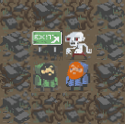
\includegraphics[width=4cm,keepaspectratio]{Images/board-reduced.png}
\end{center}

Pour la réalisation de ces diagrammes, nous avons décidé de diviser le diagramme en cinq sous-diagrammes mettant chacun l'accent sur un aspect du monde ci-dessus :
\begin{itemize}
    \item Le jeu actuellement en cours.
    \item Le plateau de jeu en lui-même.
    \item Le monde tel qu'il est perçu par l'avatar 1 (en vert).
    \item Le monde tel qu'il est perçu par l'avatar 2 (en bleu).
    \item Le monde tel qu'il est perçu par le zombie.
\end{itemize}

\section{Jeu}
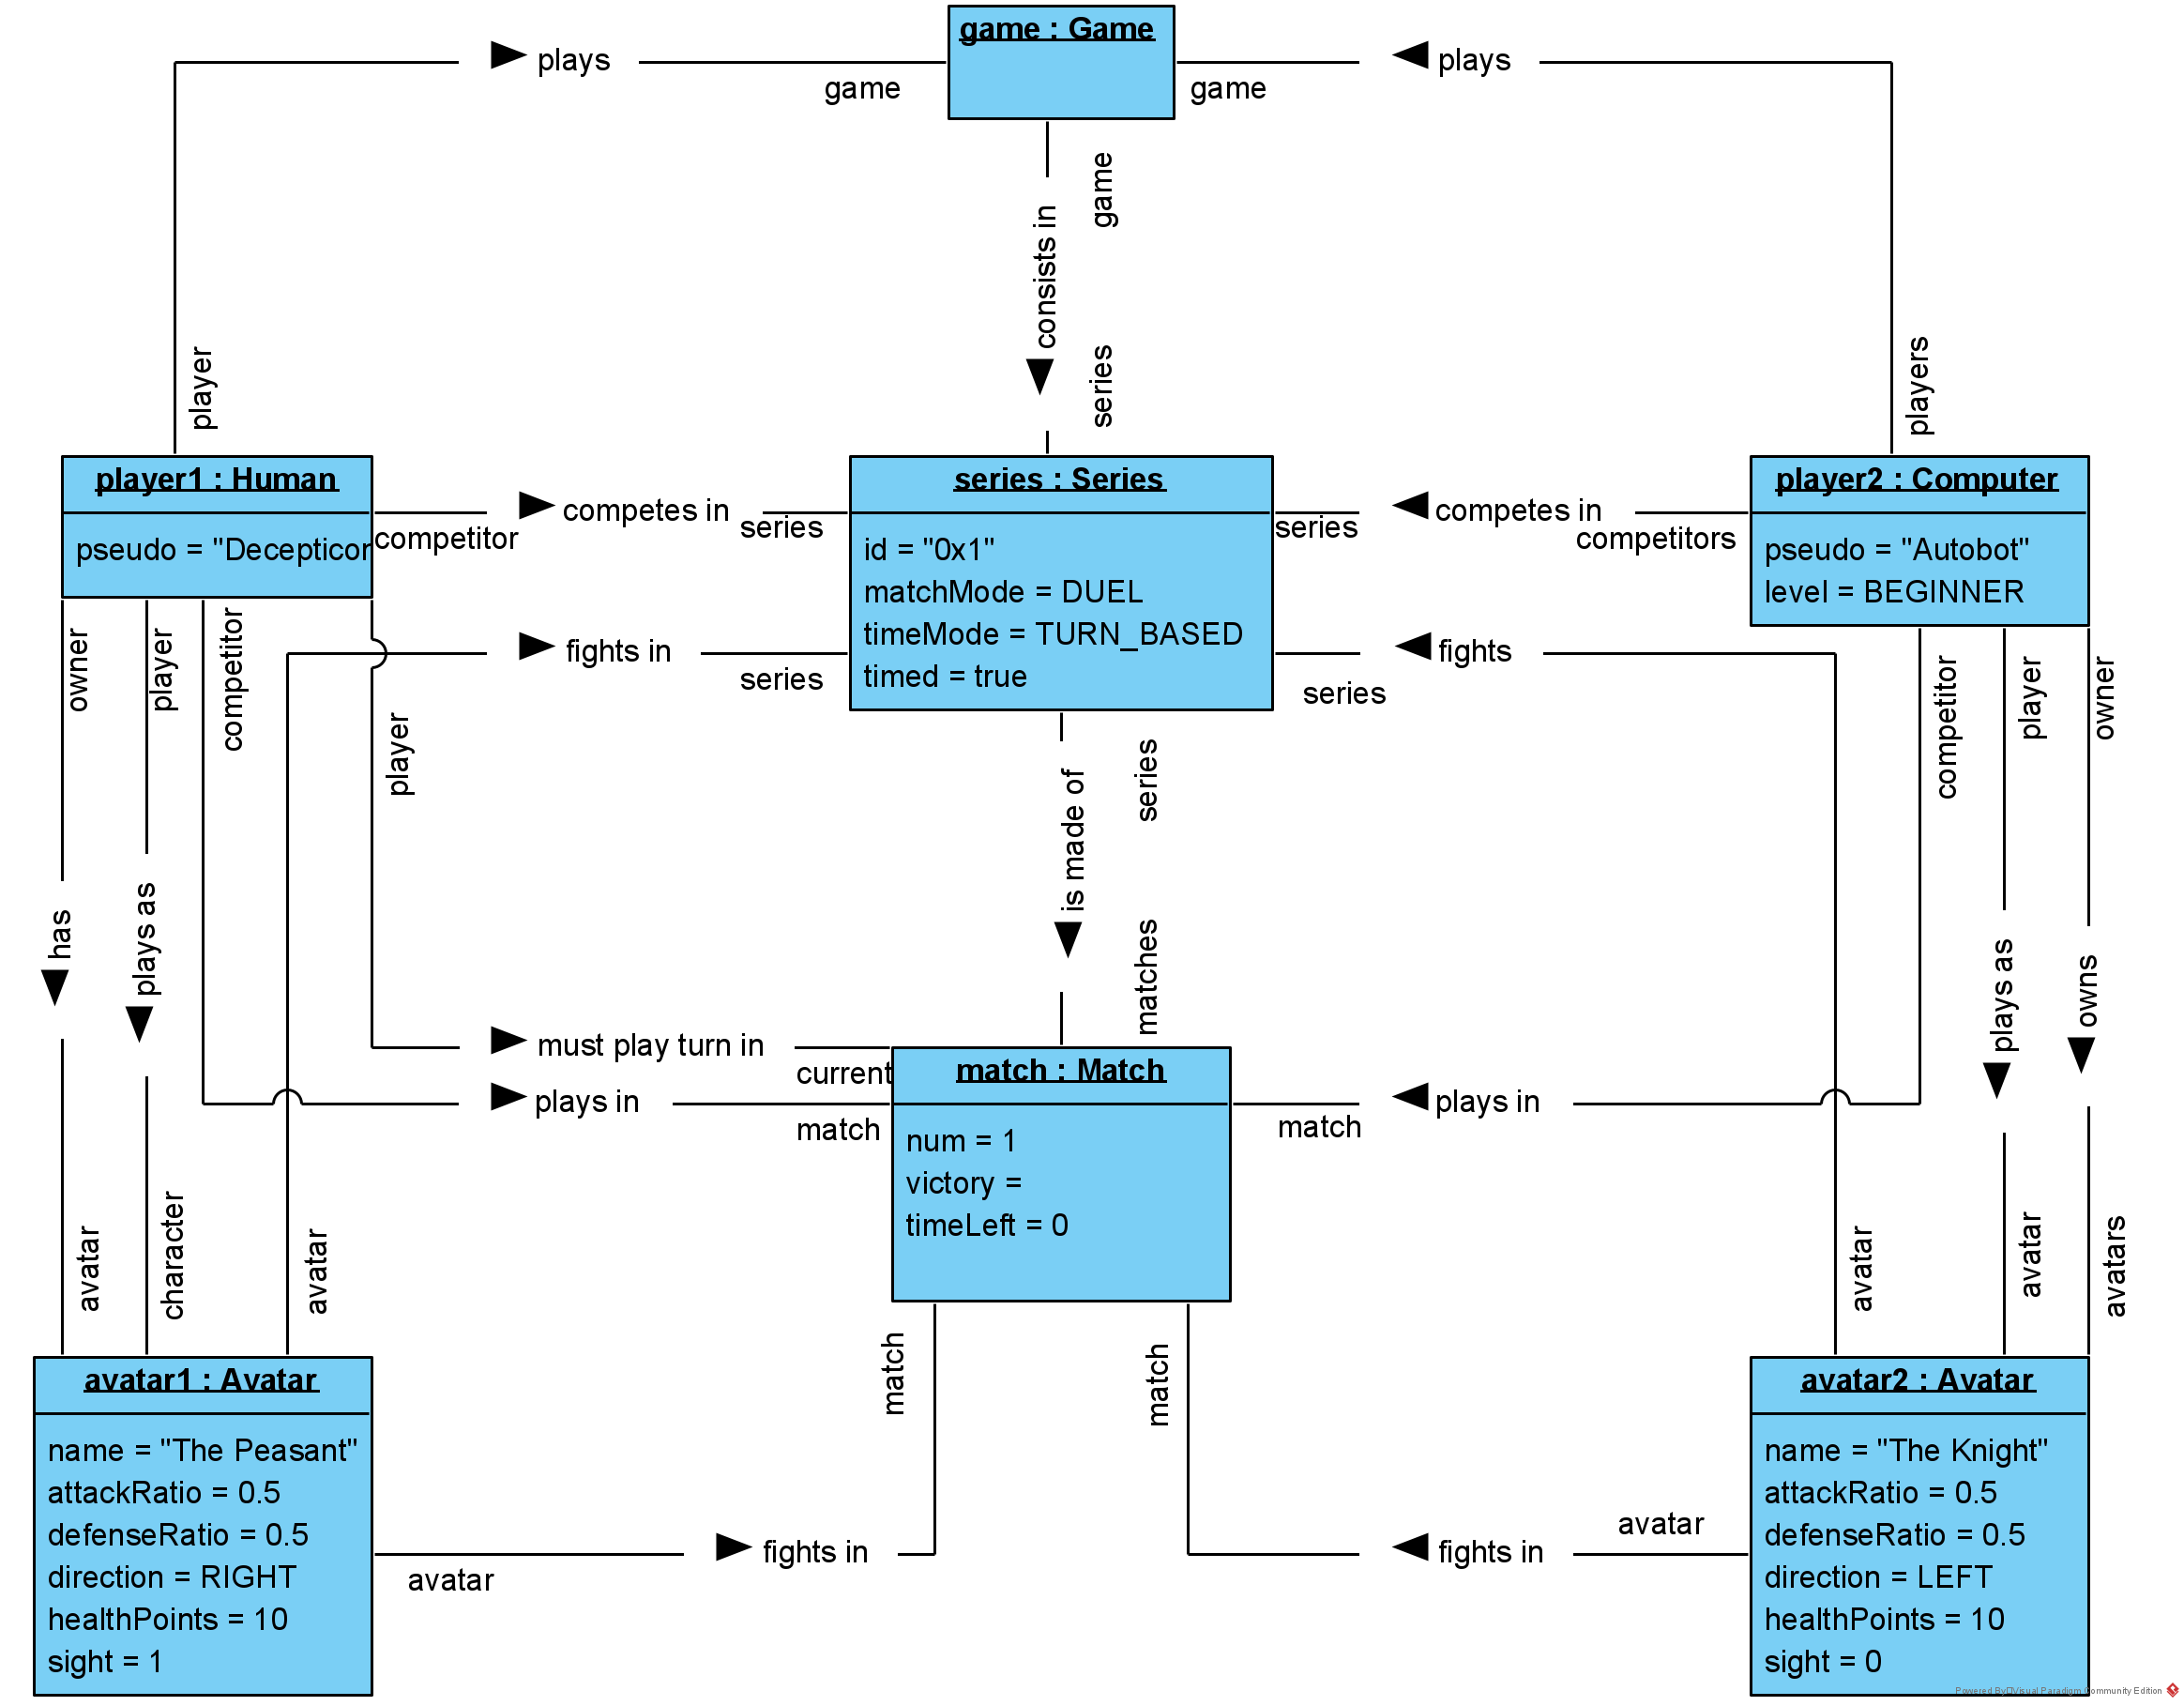
\includegraphics[width=\textwidth,height=\textheight,keepaspectratio]{Diagrams/OD-Game.png}\newline

Le jeu actuellement en cours rassemble deux joueurs :
\begin{itemize}
    \item Un joueur humain - le joueur 1.
    \item Un joueur artificiel, contrôlé par l'ordinateur - le joueur 2.
\end{itemize}

Ces deux joueurs sont engagés dans une suite de rencontres en mode DUEL, en tour-par-tour avec une limite de temps. Ils ont pour cela chacun choisi un avatar pour disputer les rencontres de cette suite. L'identifiant unique de la série est 0x1.\newline

La suite est composée d'un unique match, dans lequel sont engagés les joueurs et leurs avatars. Ce match porte le numéro unique 1, n'a pas encore été gagné (par mort subite ou découverte du Graal) et ne compte plus que 3 tours avant de s'achever.\newline

C'est au tour du joueur 1 de choisir son action pour le tour.\newline

\section{Plateau}
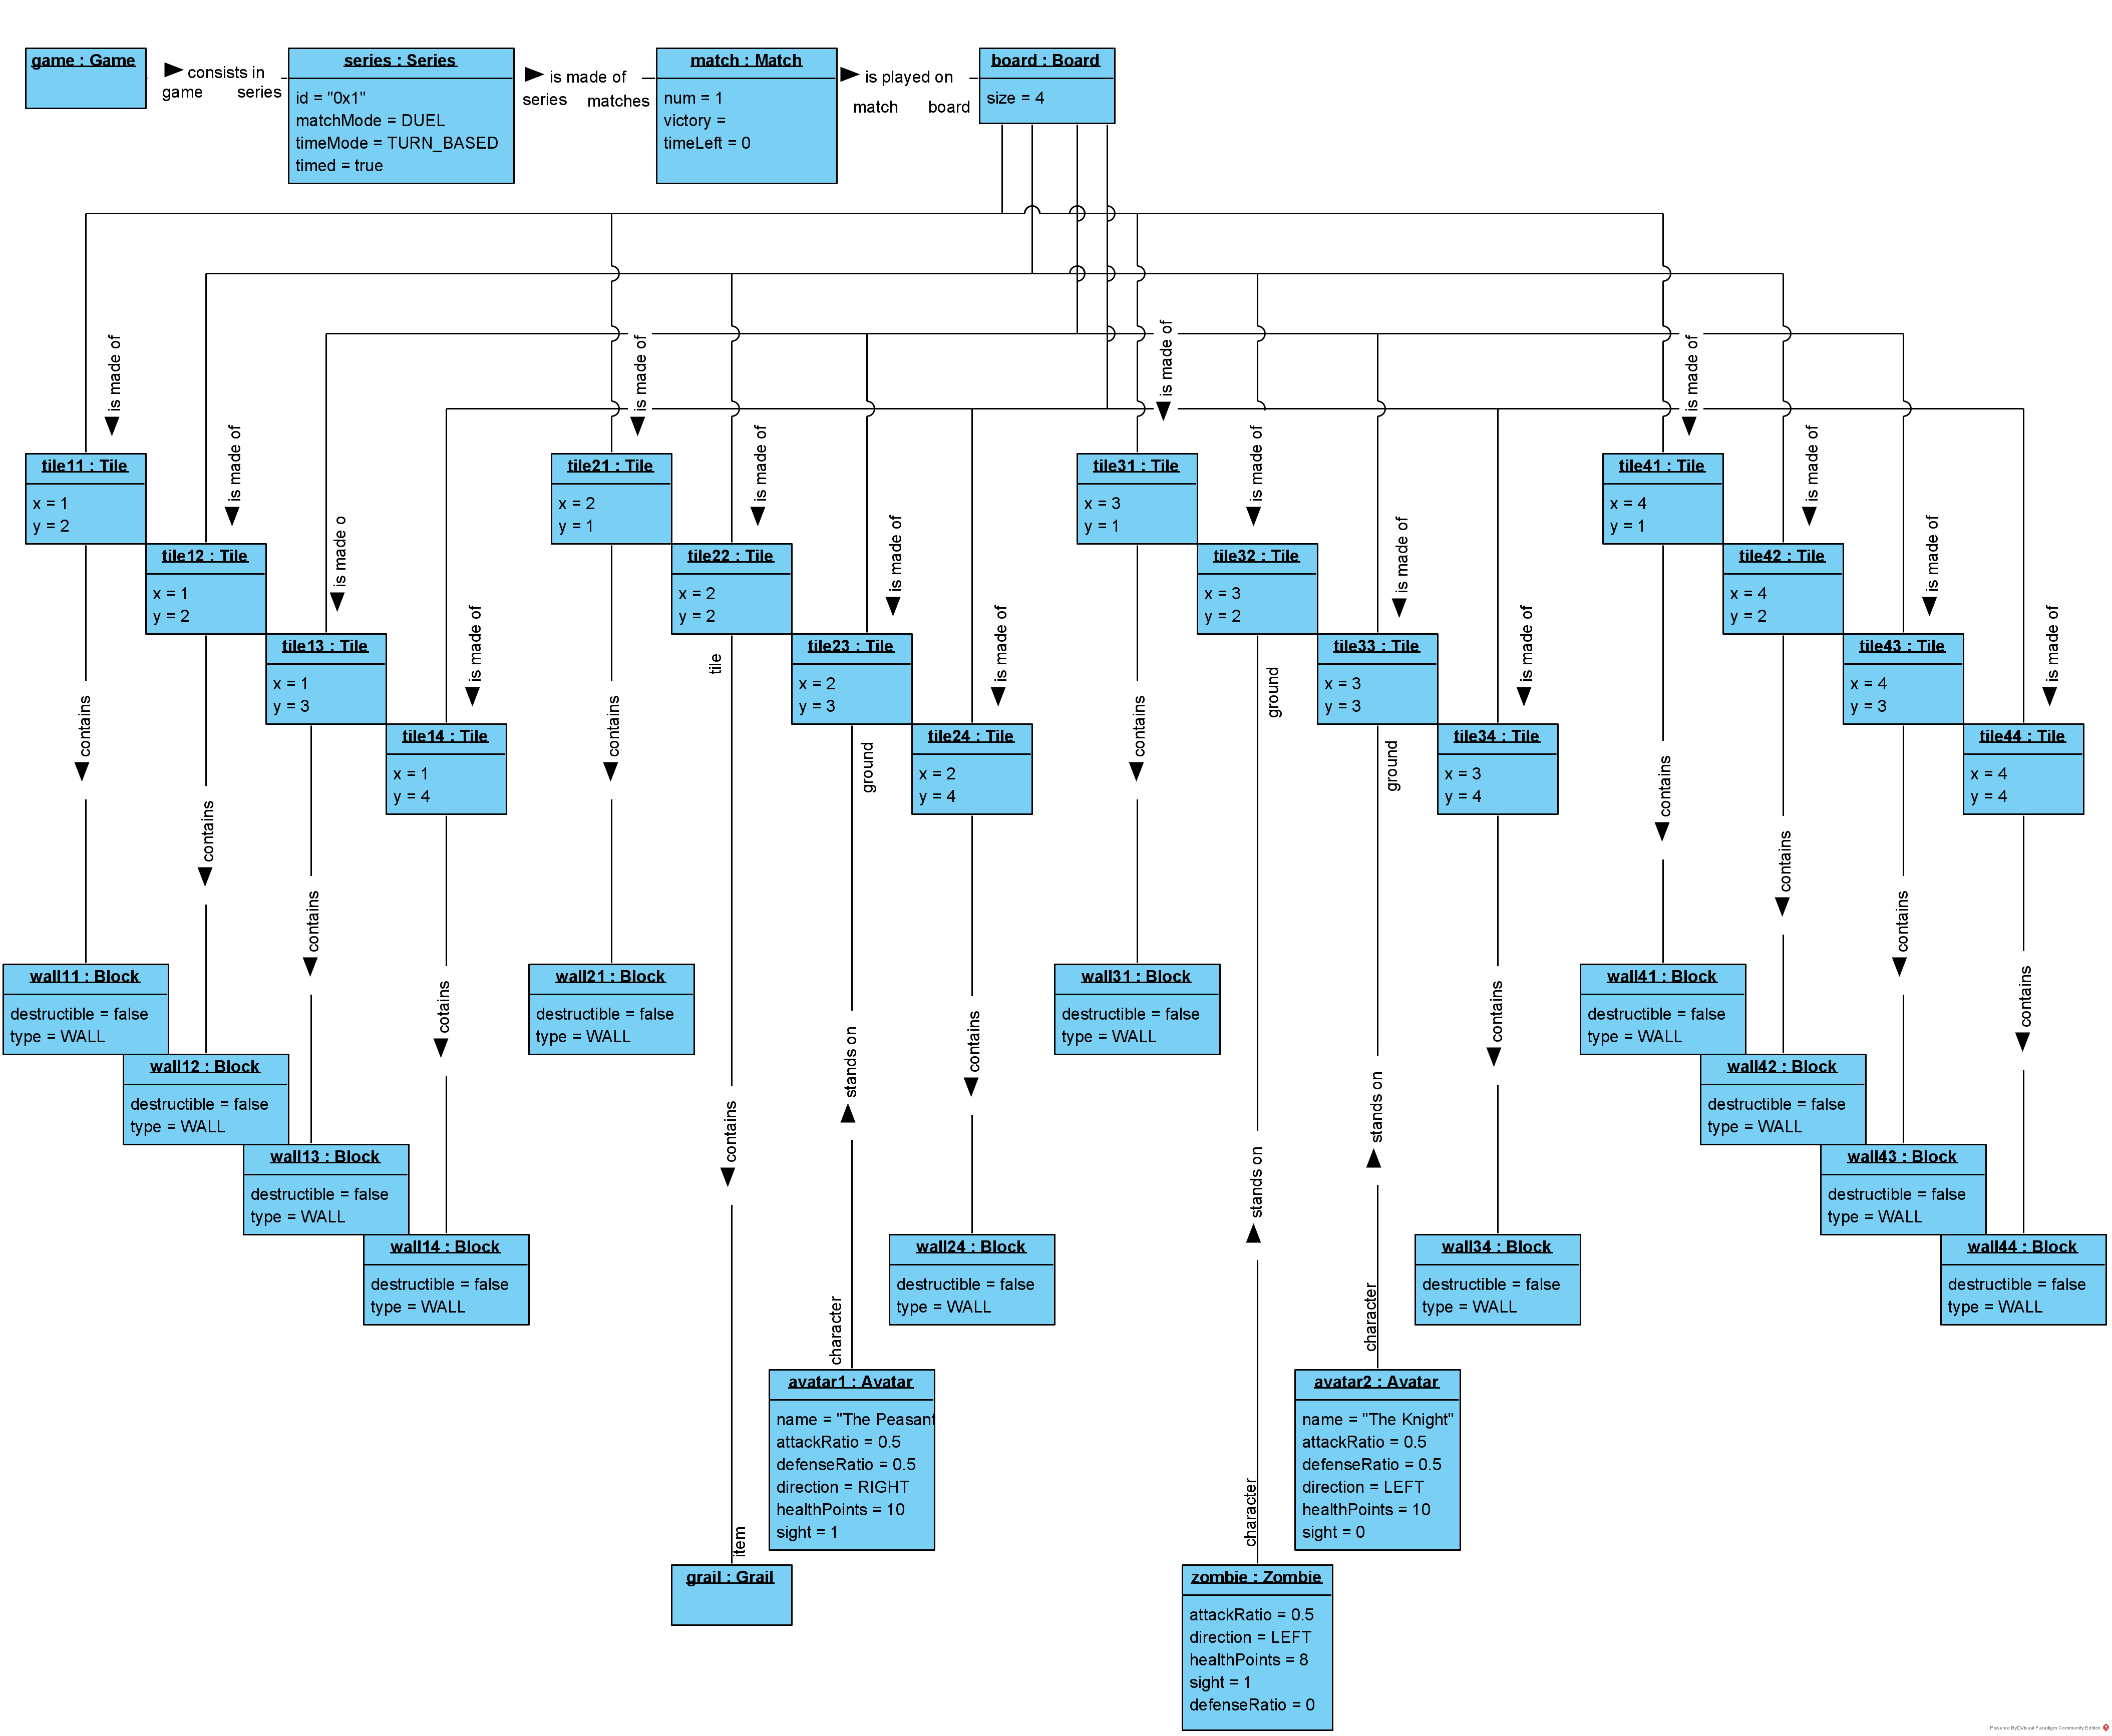
\includegraphics[width=\textheight,height=\textwidth,keepaspectratio,angle=90,origin=c]{Diagrams/OD-Board.png}\newline

Le plateau présente 16 tuiles, dont 4 servent de plateau réel de jeu.
\begin{itemize}
    \item Les bords comprennent tous un obstacle de type \textit{Block} (c'est-à-dire infranchissable et indestructible).
    \item Trois tuiles comprennent des personnages.
    \item Une tuile comprend un objet, le Graal.
\end{itemize}

    \begin{tcolorbox}
    Nous avons volontairement omis ici de préciser les éléments des relations \textit{"[1] board is made of [1..*] tiles"}, afin de ne pas surcharger le diagramme.
    \end{tcolorbox}

\section{Avatar 1}
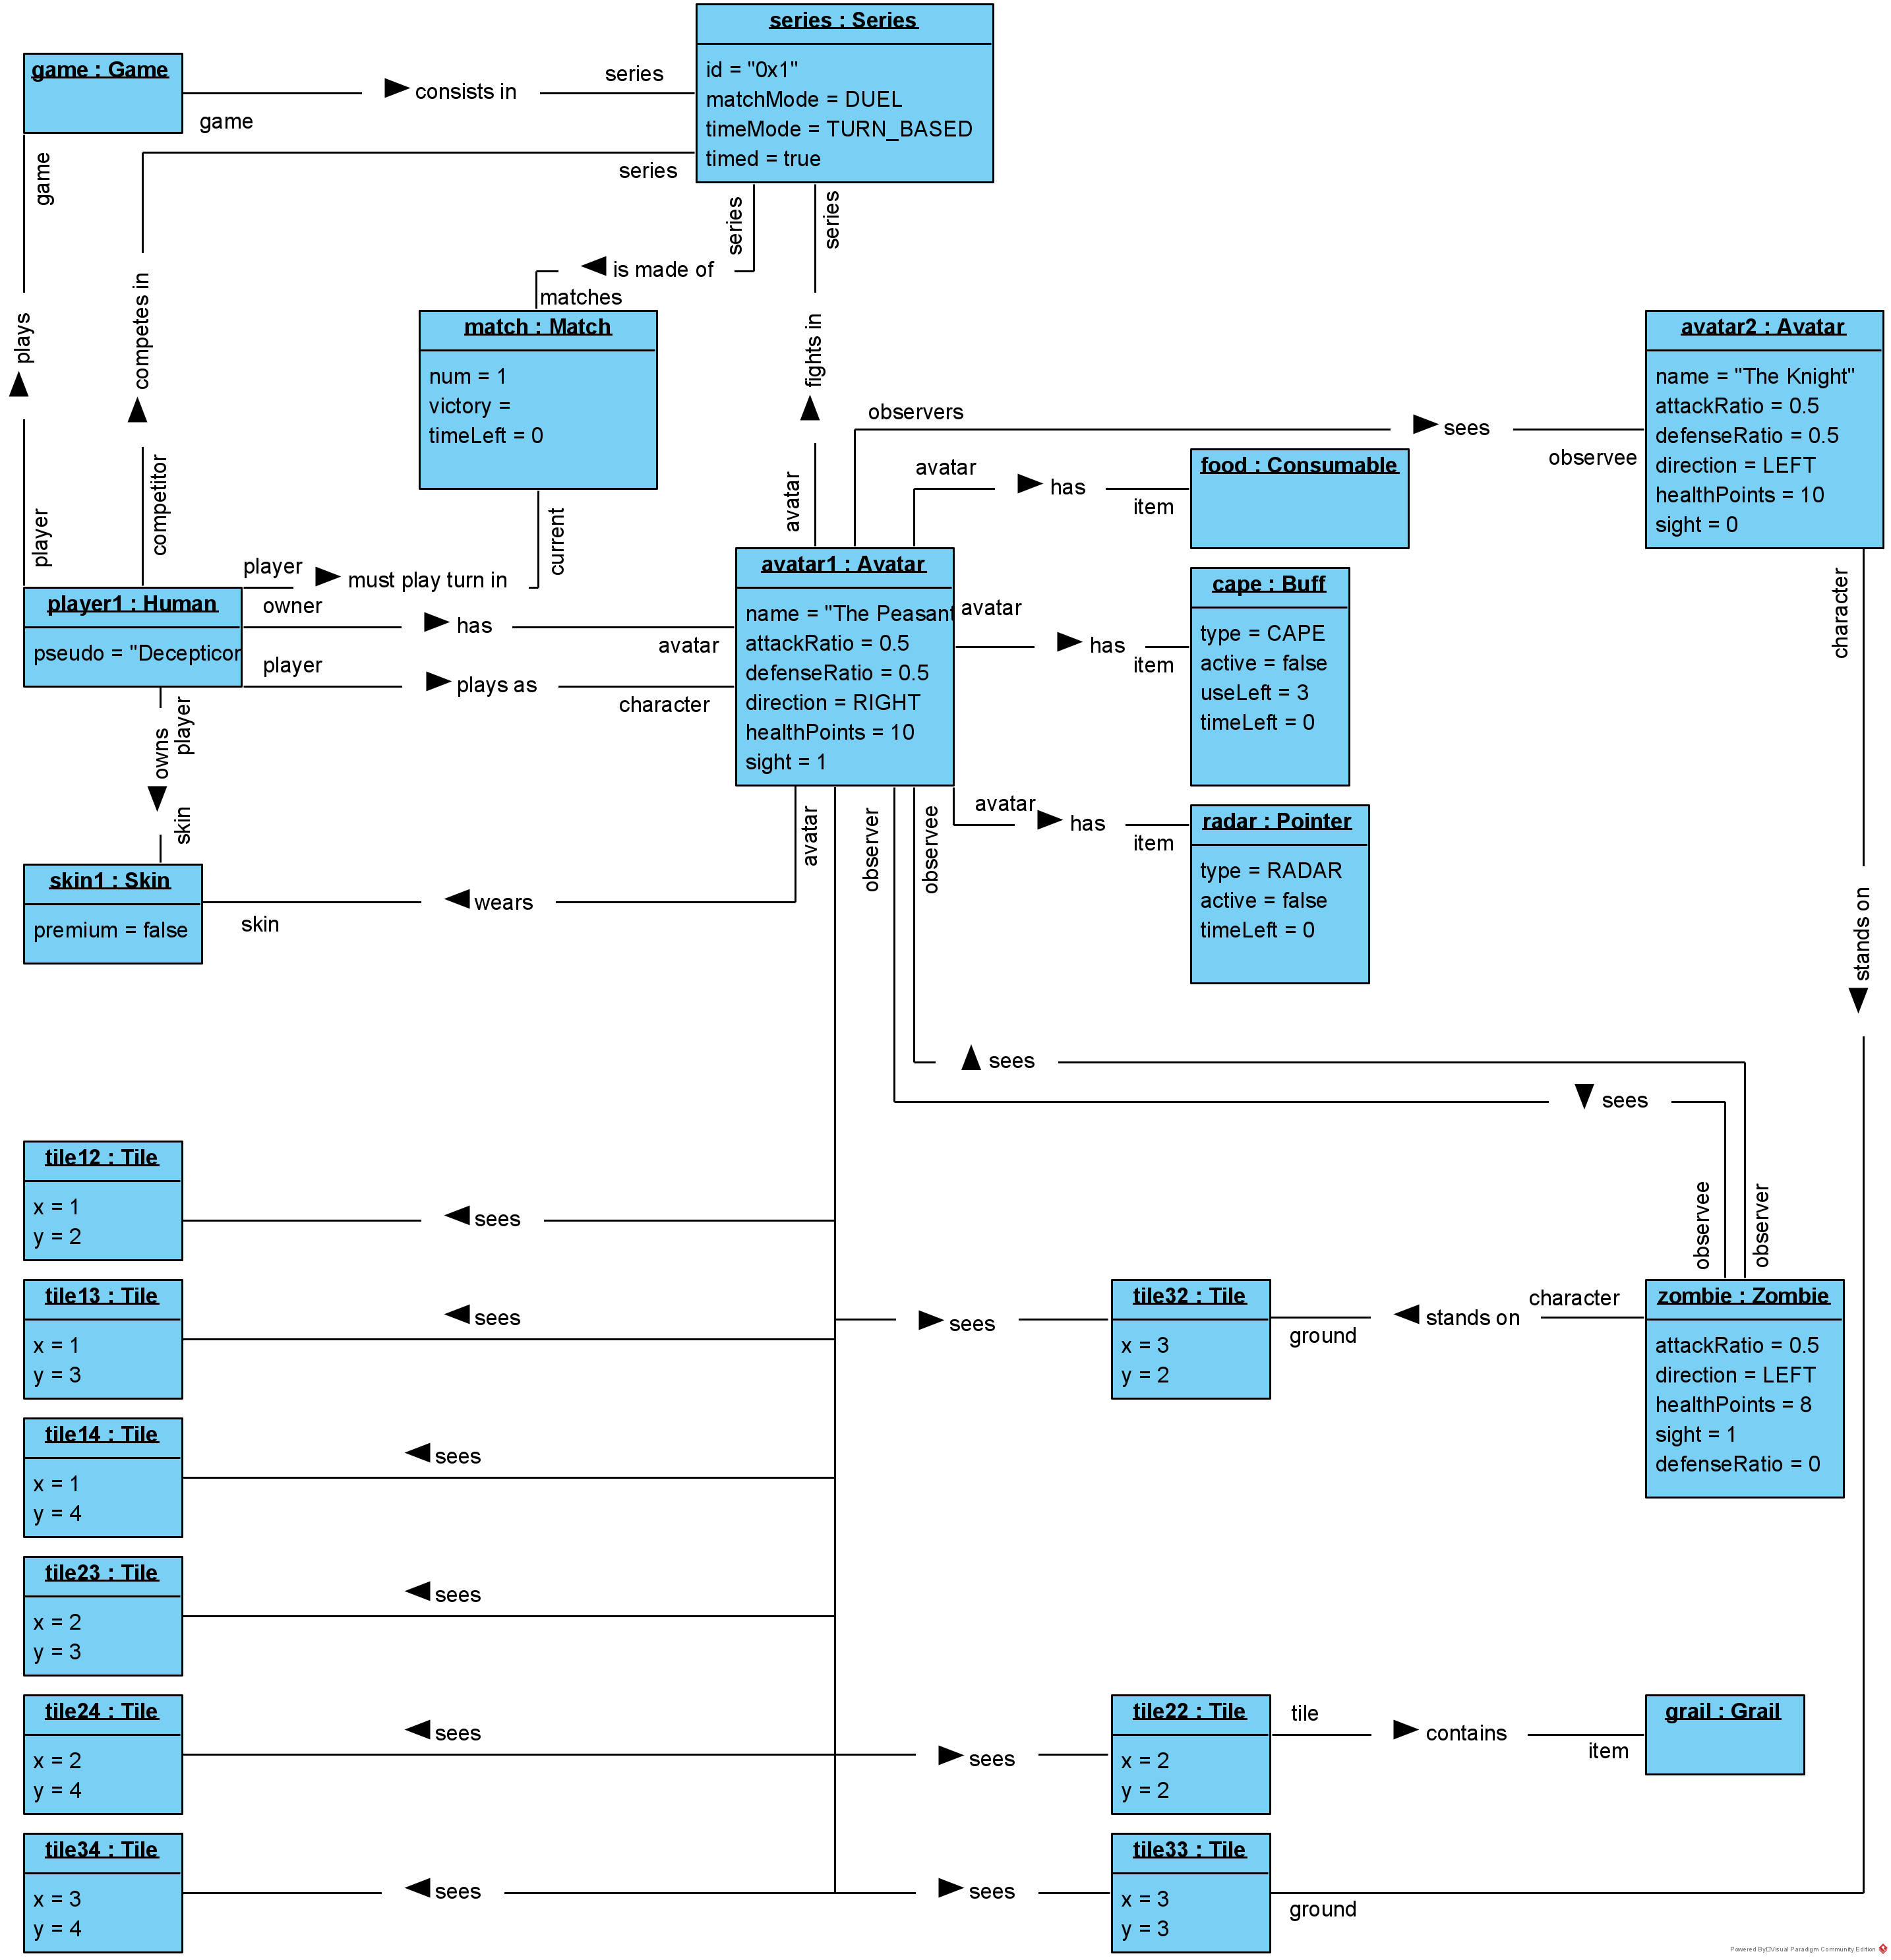
\includegraphics[width=\textwidth,height=\textheight,keepaspectratio]{Diagrams/OD-Player1.png}\newline

Le monde perçu par l'avatar 1 dépend de son indice de vision : celui-ci étant de 1, ce personnage "voit" sa tuile plus les 8 tuiles qui l'entourent. Ce faisant, il peut apercevoir l'avatar 2, le zombie et le Graal.\newline

L'avatar utilise l'apparence par défaut, non-payante et a un inventaire constitué de 1 nourriture, une cape de mage avec 3 points d'utilisation et 9 tours restants et encore 10 points de vie. Il possède également un objet-radar dont il reste 1 tour.\newline

Il porte en outre le nom de \textit{The Peasant} et présente les ratios AP=0.5 et DP=0.5 et un solde de points de vie de 10. N'ayant pas encore pu faire de déplacement, sa direction a été arbitrairement initialisée à \textit{Direction.RIGHT}.\newline

Ce personnage est contrôlé par le joueur 1, dont c'est le tour de jouer.

    \begin{tcolorbox}
    Nous avons volontairement omis ici de préciser les éléments des relations \textit{"[0..*] observers sees [1..*] tiles"}, afin de ne pas surcharger le diagramme.
    \end{tcolorbox}

\section{Avatar 2}
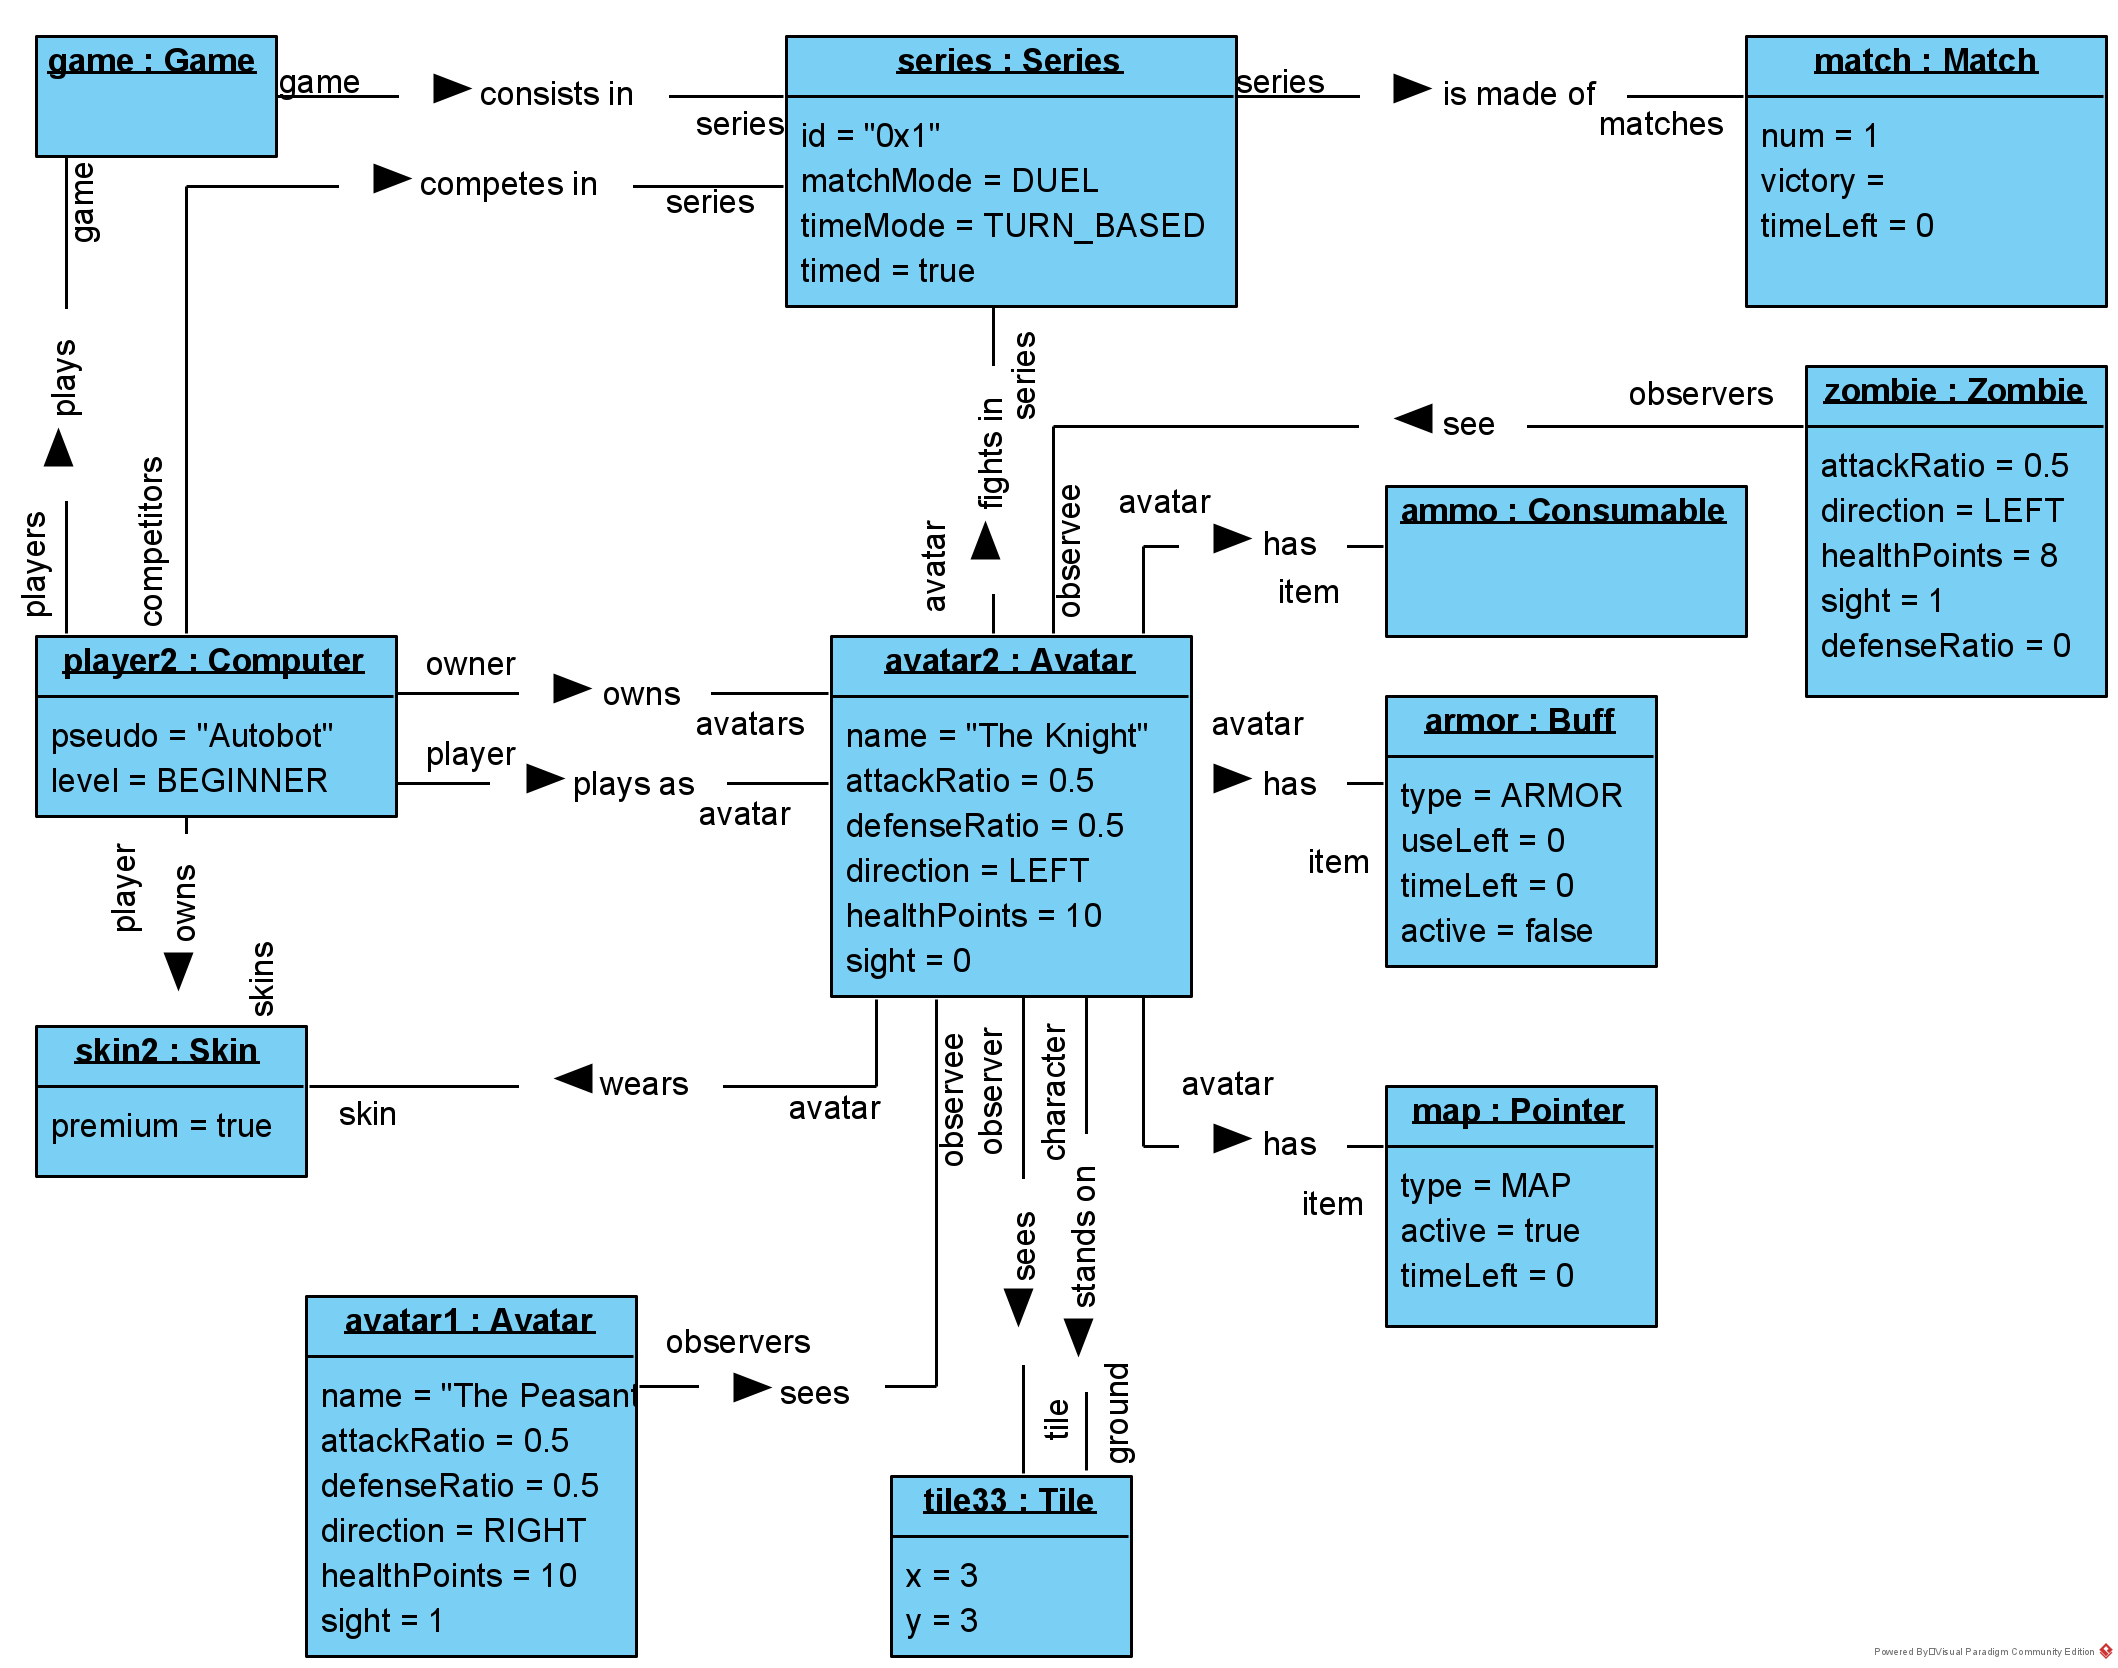
\includegraphics[width=\textwidth,height=\textheight,keepaspectratio]{Diagrams/OD-Player2.png}\newline

Le monde perçu par l'avatar 2 est beaucoup plus restreint, puisque son indice de vision est 0 : il ne voit par conséquent que la tuile sur laquelle il est positionné. Ceci ne l'empêche pas d'être vu à la fois par le zombie et l'avatar 1 (qui possèdent une plus grand portée de vue).\newline

Ce personnage, dénommé \textit{The Knight}, porte une apparence \textit{Premium}, possédé par le joueur 2. Il possède en outre dans son inventaire une munition, une cotte de maille encore non-utilisée et un pointeur vers le Graal automatiquement activé (et sans limite d'utilisation).\newline

Tout comme l'avatar 1, il présente les ratios AP=0.5 et DP=0.5 et un solde de points de vie de 10. Sa direction a également été posée arbitrairement comme \textit{Direction.LEFT}.\newline

Cet avatar est contrôlé par l'ordinateur et ne devrait pas poser un gros challenge (son niveau est débutant).

    \begin{tcolorbox}
    Nous avons volontairement omis ici de préciser les éléments des relations \textit{"[0..*] observers sees [1..*] tiles"}, afin de ne pas surcharger le diagramme.
    \end{tcolorbox}

\section{zombie}
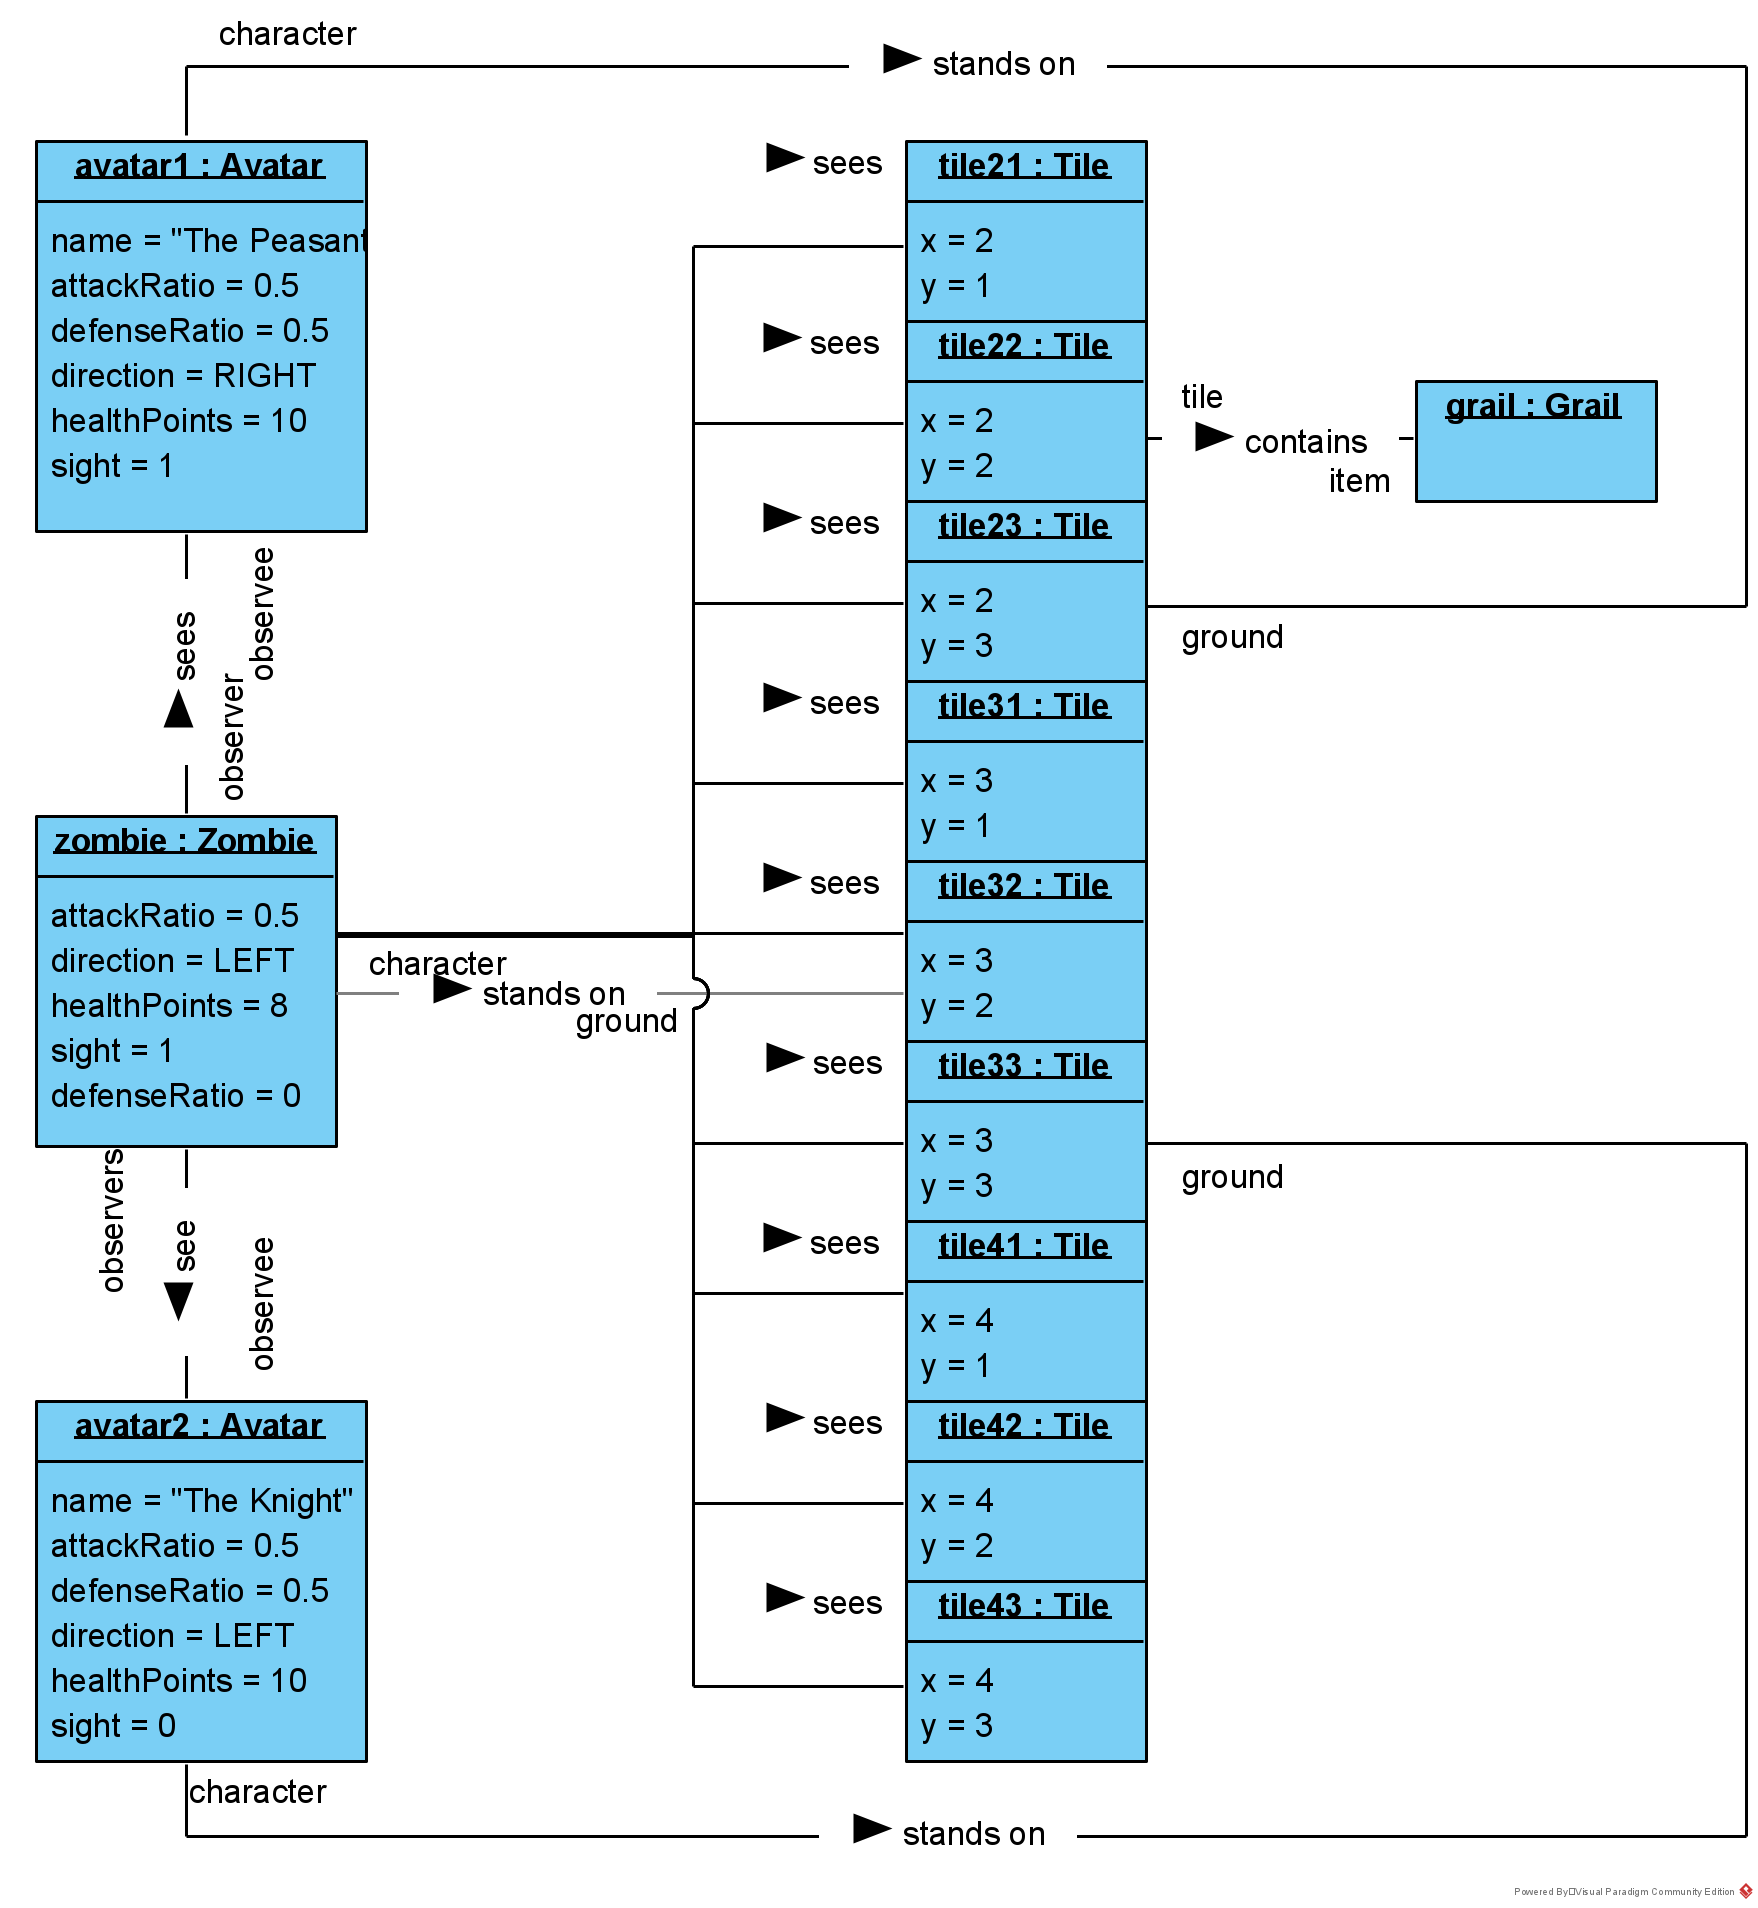
\includegraphics[width=\textwidth,height=\textheight,keepaspectratio]{Diagrams/OD-Zombie.png}\newline

Le zombie est pour sa part doté des caractéristiques suivantes : AP=0.5, DP=0;5, direction arbitraire vers la gauche. Il voit les deux personnages contrôlés par les joueurs, ainsi que 9 tuiles dont l'une contient le Graal.

    \begin{tcolorbox}
    Nous avons volontairement omis ici de préciser les éléments des relations \textit{"[0..*] observers sees [1..*] tiles"}, afin de ne pas surcharger le diagramme.
    \end{tcolorbox}

\newpage
\chapter{Description des stratégies}

\section{Pré-version}

\textbf{Question 4.7.}\label{Question 4.7.}\newline
 
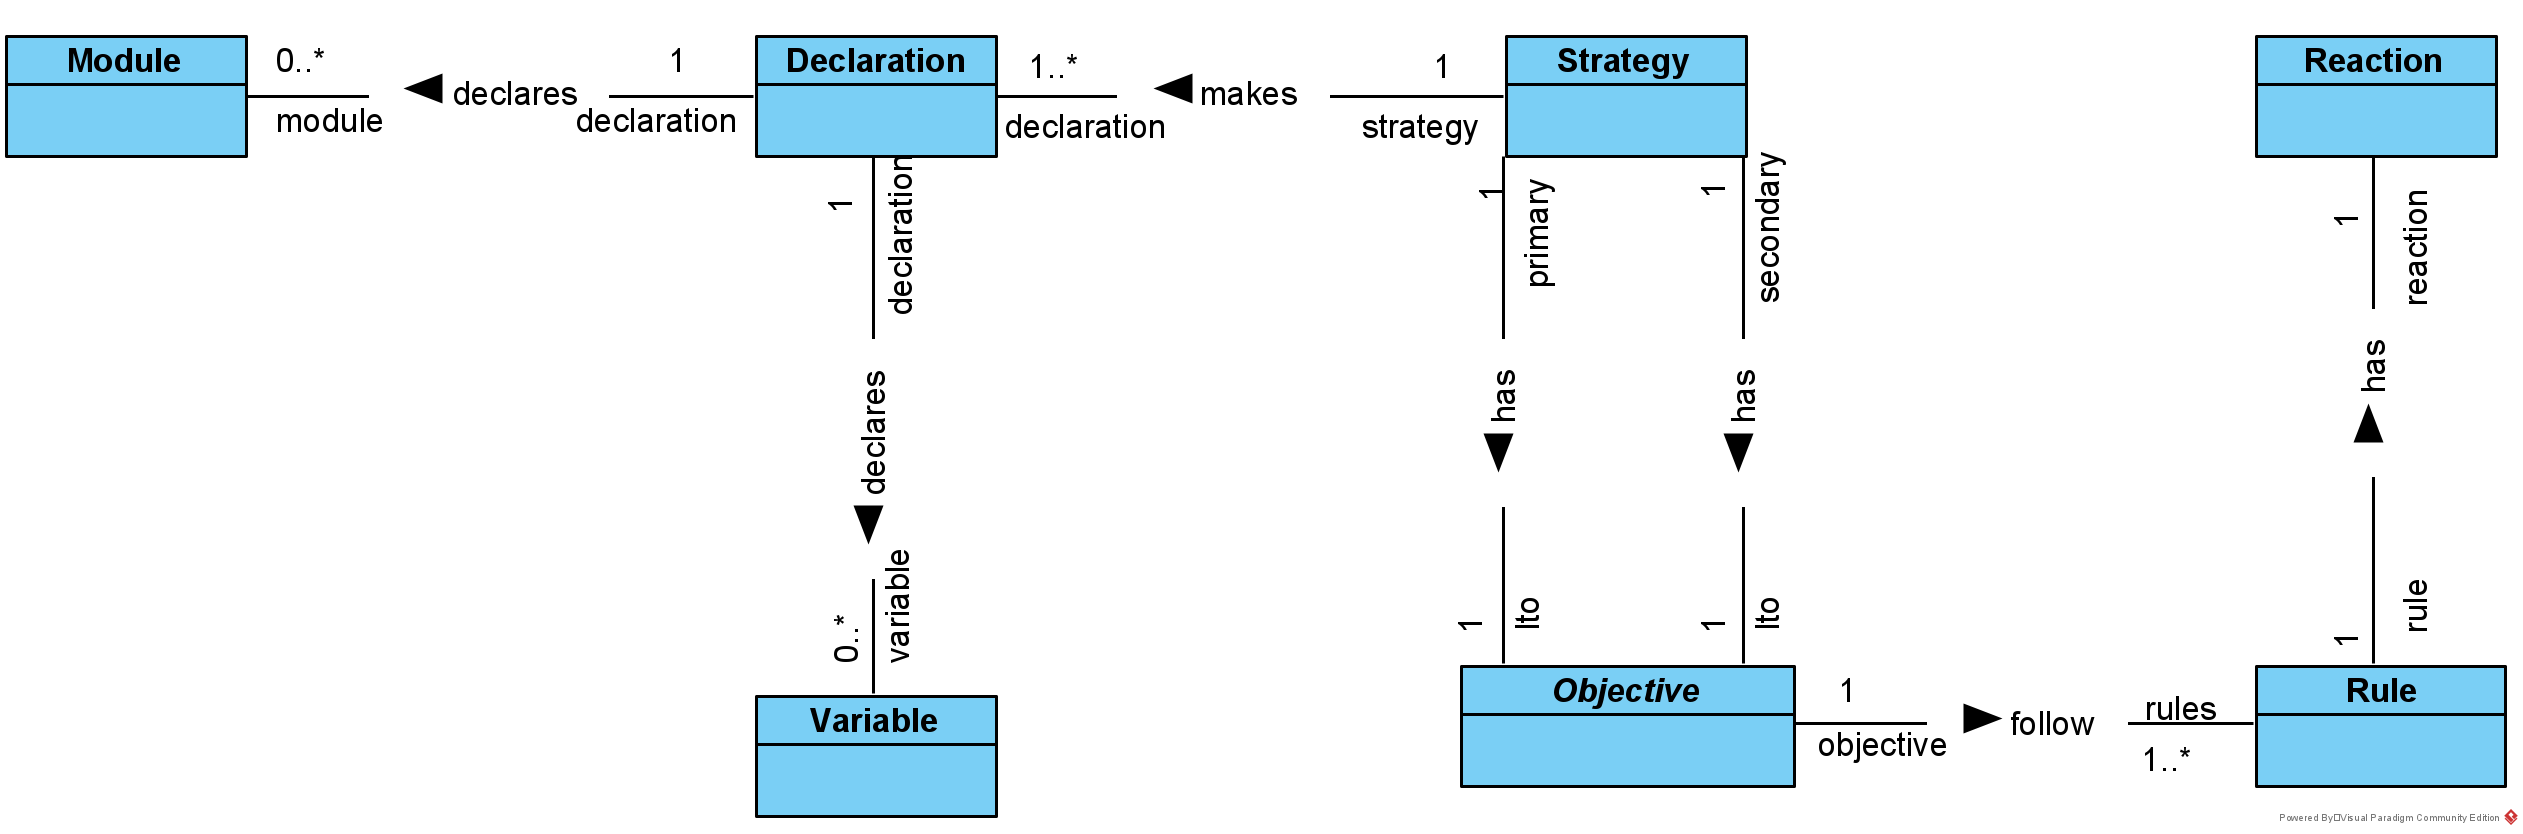
\includegraphics[width=\textwidth,height=\textheight,keepaspectratio]{Diagrams/DS-preversion.png}\newline

Les stratégies décrivent les mécanismes d'instructions et de réalisation de comportements automatisés au sein du jeu. Un personnage se voit ainsi attribuer une stratégie qui va guider le sens de ses actions et lui donner une série d'outils pour les mener à bien. On distingue ainsi les objectifs (primaires et secondaires) qui vont prescrire un comportement général et donner une série de directives pour réagir à certaines circonstances, et les modules qui sont des descriptions de sous-comportements.

\section{Version détaillée}
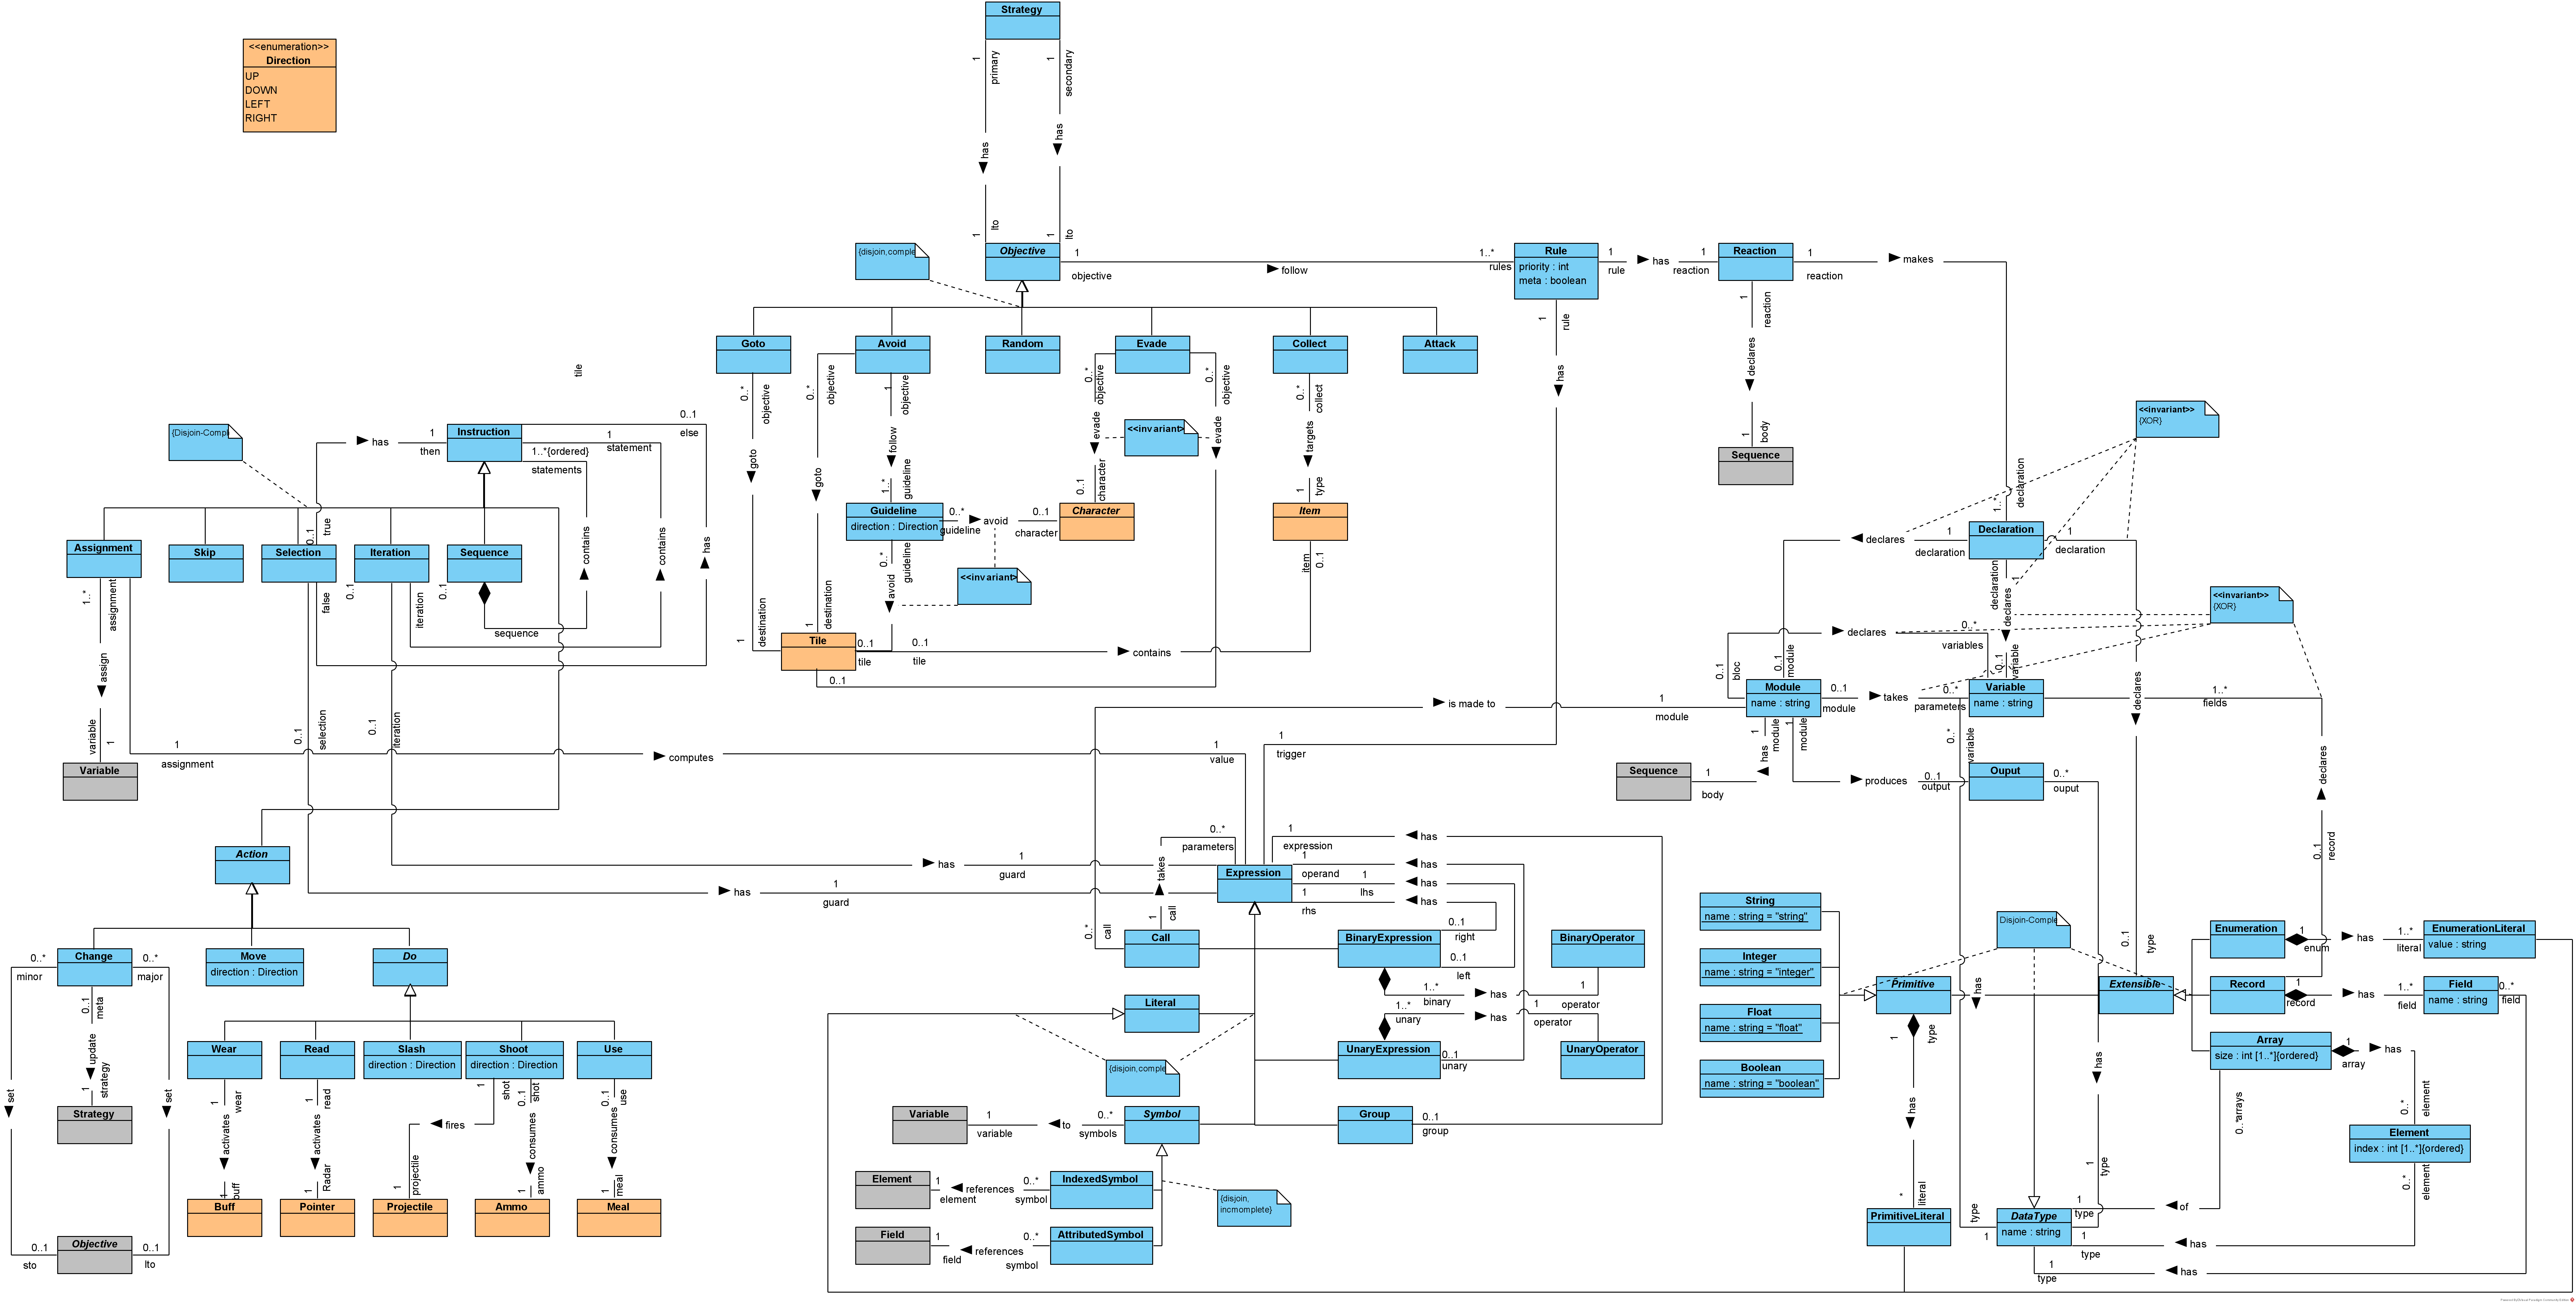
\includegraphics[width=.95\textheight,height=\textwidth,keepaspectratio,angle=90,origin=c]{Diagrams/DS-fullversion.png}\newline

(En orange sont les classes issues du modèle de jeu, et en gris sont les classes qui ont été dupliquées pour permettre la réalisation d'un diagramme lisible).\newline

Dans cette section, nous détaillerons les diagrammes spécifiques aux différentes composantes de la définition des stratégies.

\subsection{Définition}

\subsubsection{Stratégie et directives}

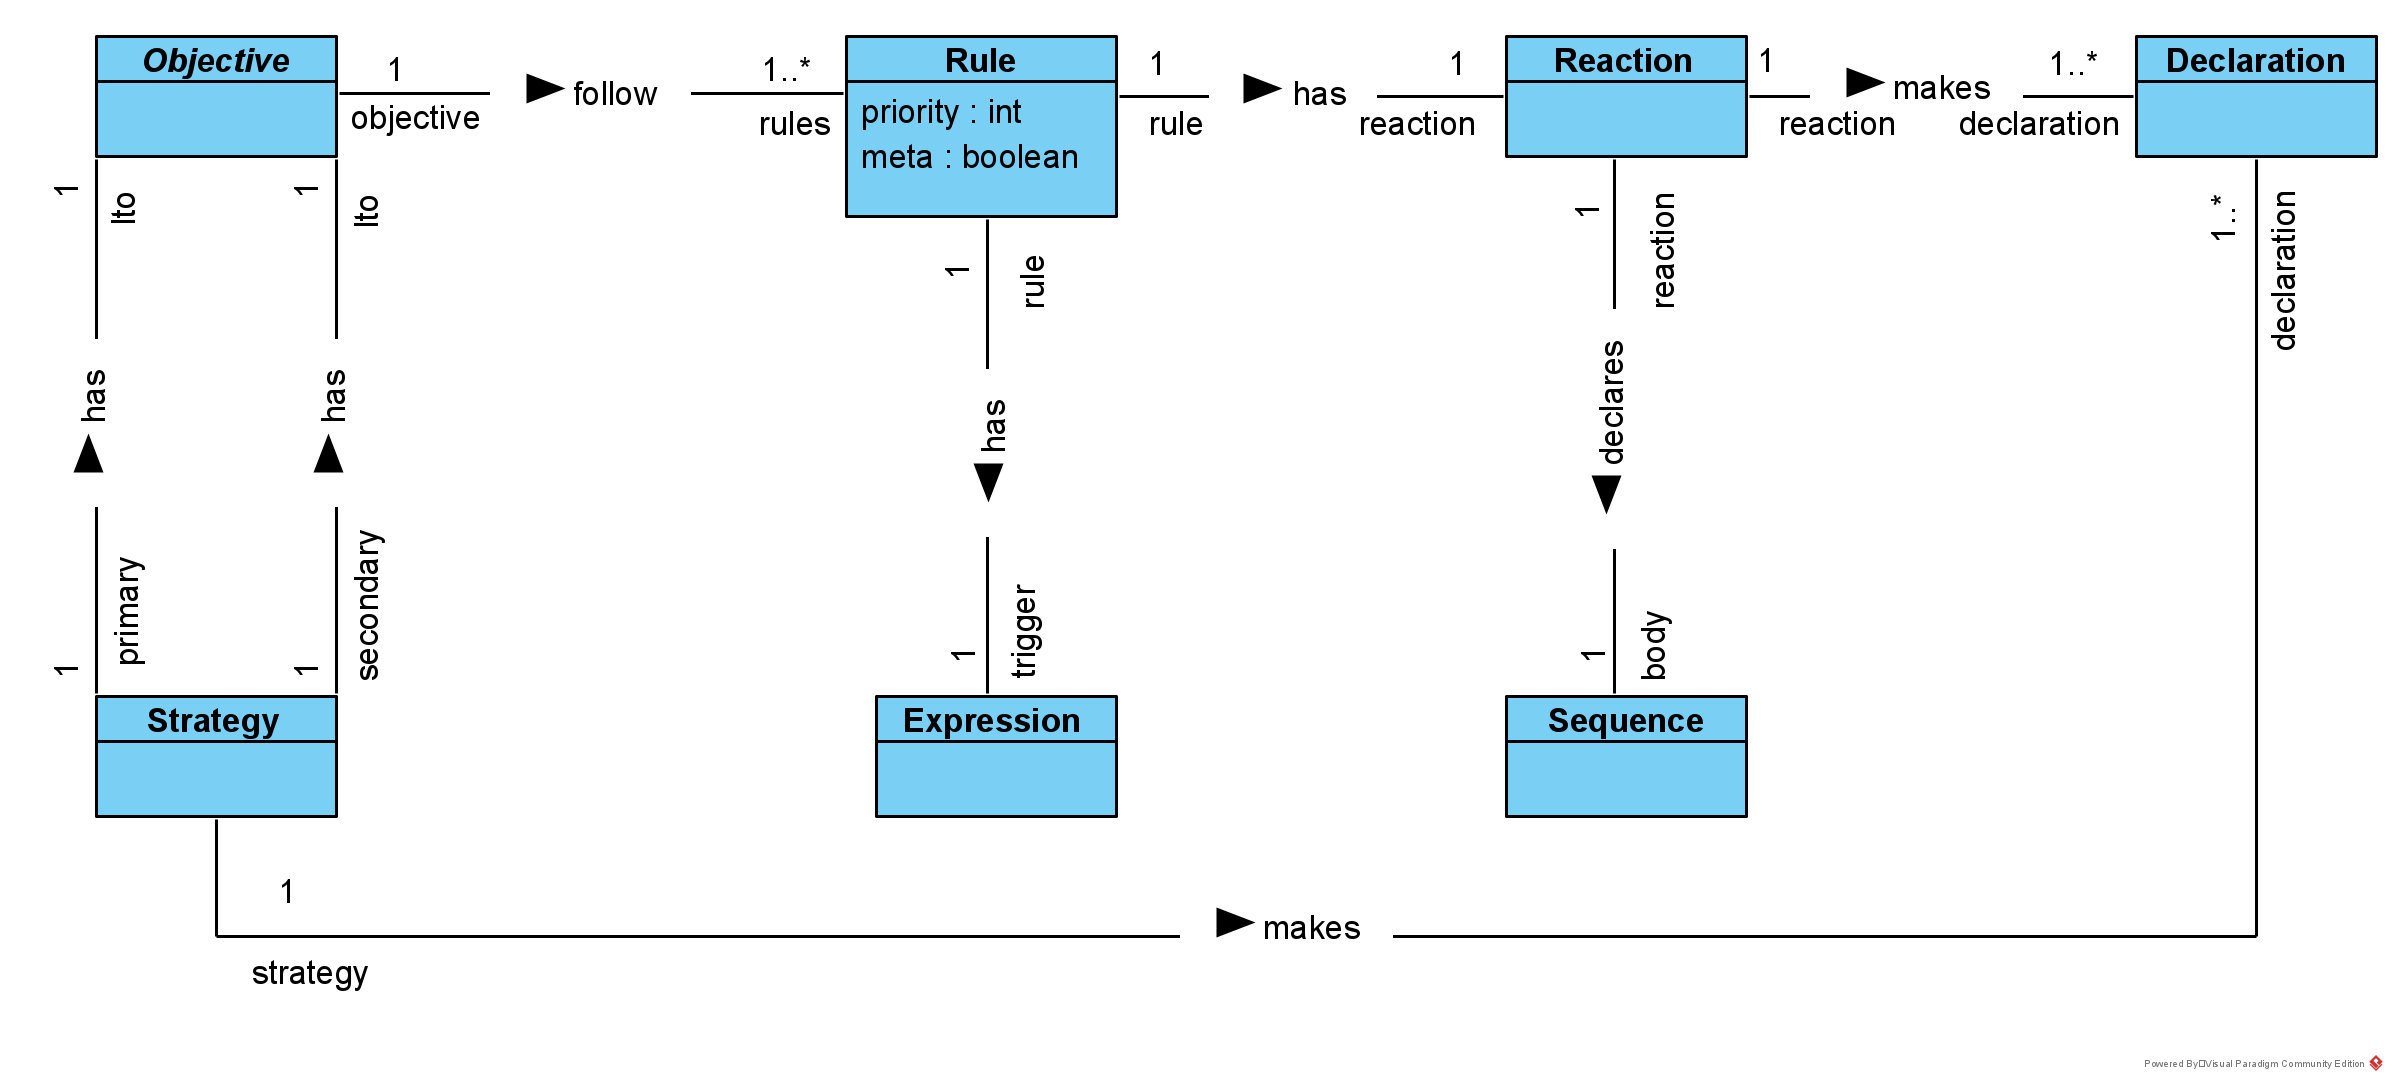
\includegraphics[width=\textwidth,height=\textheight,keepaspectratio]{Diagrams/DS-Strategy.png}\newline

Les stratégies permettent de décrire le comportement prescrit à un personnage au cours d'une rencontre durant laquelle ce personnage est contrôlé automatiquement.
Elles se composent de deux aspects :
\begin{itemize}
    \item Un objectif principal (\textit{Long-Term Objective - LTO}), qui sert de fil rouge et reste globalement stable.
    \item Un objectif secondaire (\textit{Short-Term Objective - STO}), déclaré en fonction des conditions avoisinantes.
\end{itemize}

Au moment d'agir, le personnage fait l'état de ses objectifs : l'objectif secondaire étant présumé plus rapide à exécuter, celui-ci sera prioritaire dans l'exécution par rapport à l'objectif principal. Si l'objectif secondaire est atteint, alors le personnage peut soit en changer, soit se concentrer sur son objectif principal.\newline

Pour réaliser un objectif, un personnage suivra un ensemble de directives : un ensemble de comportements spécifiques à activer lorsque les conditions le permettent.
Nous avons ainsi les trois éléments suivants :
\begin{itemize}
    \item Le déclencheur / la garde : une expression permettant de vérifier si les conditions sont réunies pour l'exécution.
    \item La réaction / le corps : une suite d'instructions permettant de réaliser le comportement.
    \item La priorité : un marqueur permettant de déterminer la directive à appliquer en cas de conflit entre plusieurs directives activées simultanément. 
\end{itemize}

La directive choisie permet alors au personnage de réaliser un ensemble de comportements qu'elle documente dans une déclaration : elle fournit ainsi des variables significatives et des actions concrètes qui prendront le parti de ces variables.\newline

\begin{samepage}
Décrivons ici la stratégie suivie par les zombies à titre d'exemple.

\begin{center}
    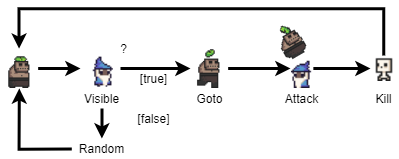
\includegraphics[width=7cm,keepaspectratio]{Images/Pseudo-activity.png}
\end{center}
\end{samepage}

Les zombies poursuivent un objectif principal clair : tuer tous les humains (qu'ils soient contrôlés par un joueur ou un ordinateur). Il s'agit d'un objectif de \textit{long-terme}, qui ne peut être réalisé si aucun humain n'est à proximité. Face à cela, les zombies adoptent en objectif secondaire de trouver les humains. Ils errent de manière aléatoire sur le plateau jusqu'à ce qu'ils croisent un personnage. Dès cet instant, l'objectif secondaire d'errance change pour intimer aux zombies de se rapprocher du personnage (de manière à pouvoir le mordre). Ce nouvel objectif s'accompagne de variables et d'actions très concrètes : information sur la position du personnage, choix de l'itinéraire le plus approprié pour s'en rapprocher, comment réagir face à un obstacle,etc. Les zombies se mettent alors en chasse du joueur jusqu'à l'atteindre. 

Dès le moment où les zombies ont atteint le personnage, tous les objectifs secondaires sont remplis et les zombies peuvent alors appliquer leur objectif principal : \textit{kill all humans}. Ils retournent enfin à leur phase d'errance et se remettent à chercher une nouvelle victime.

\subsubsection{Objectif}

\textbf{Question 4.10.}\label{Question 4.10.}\newline

\nopagebreak 

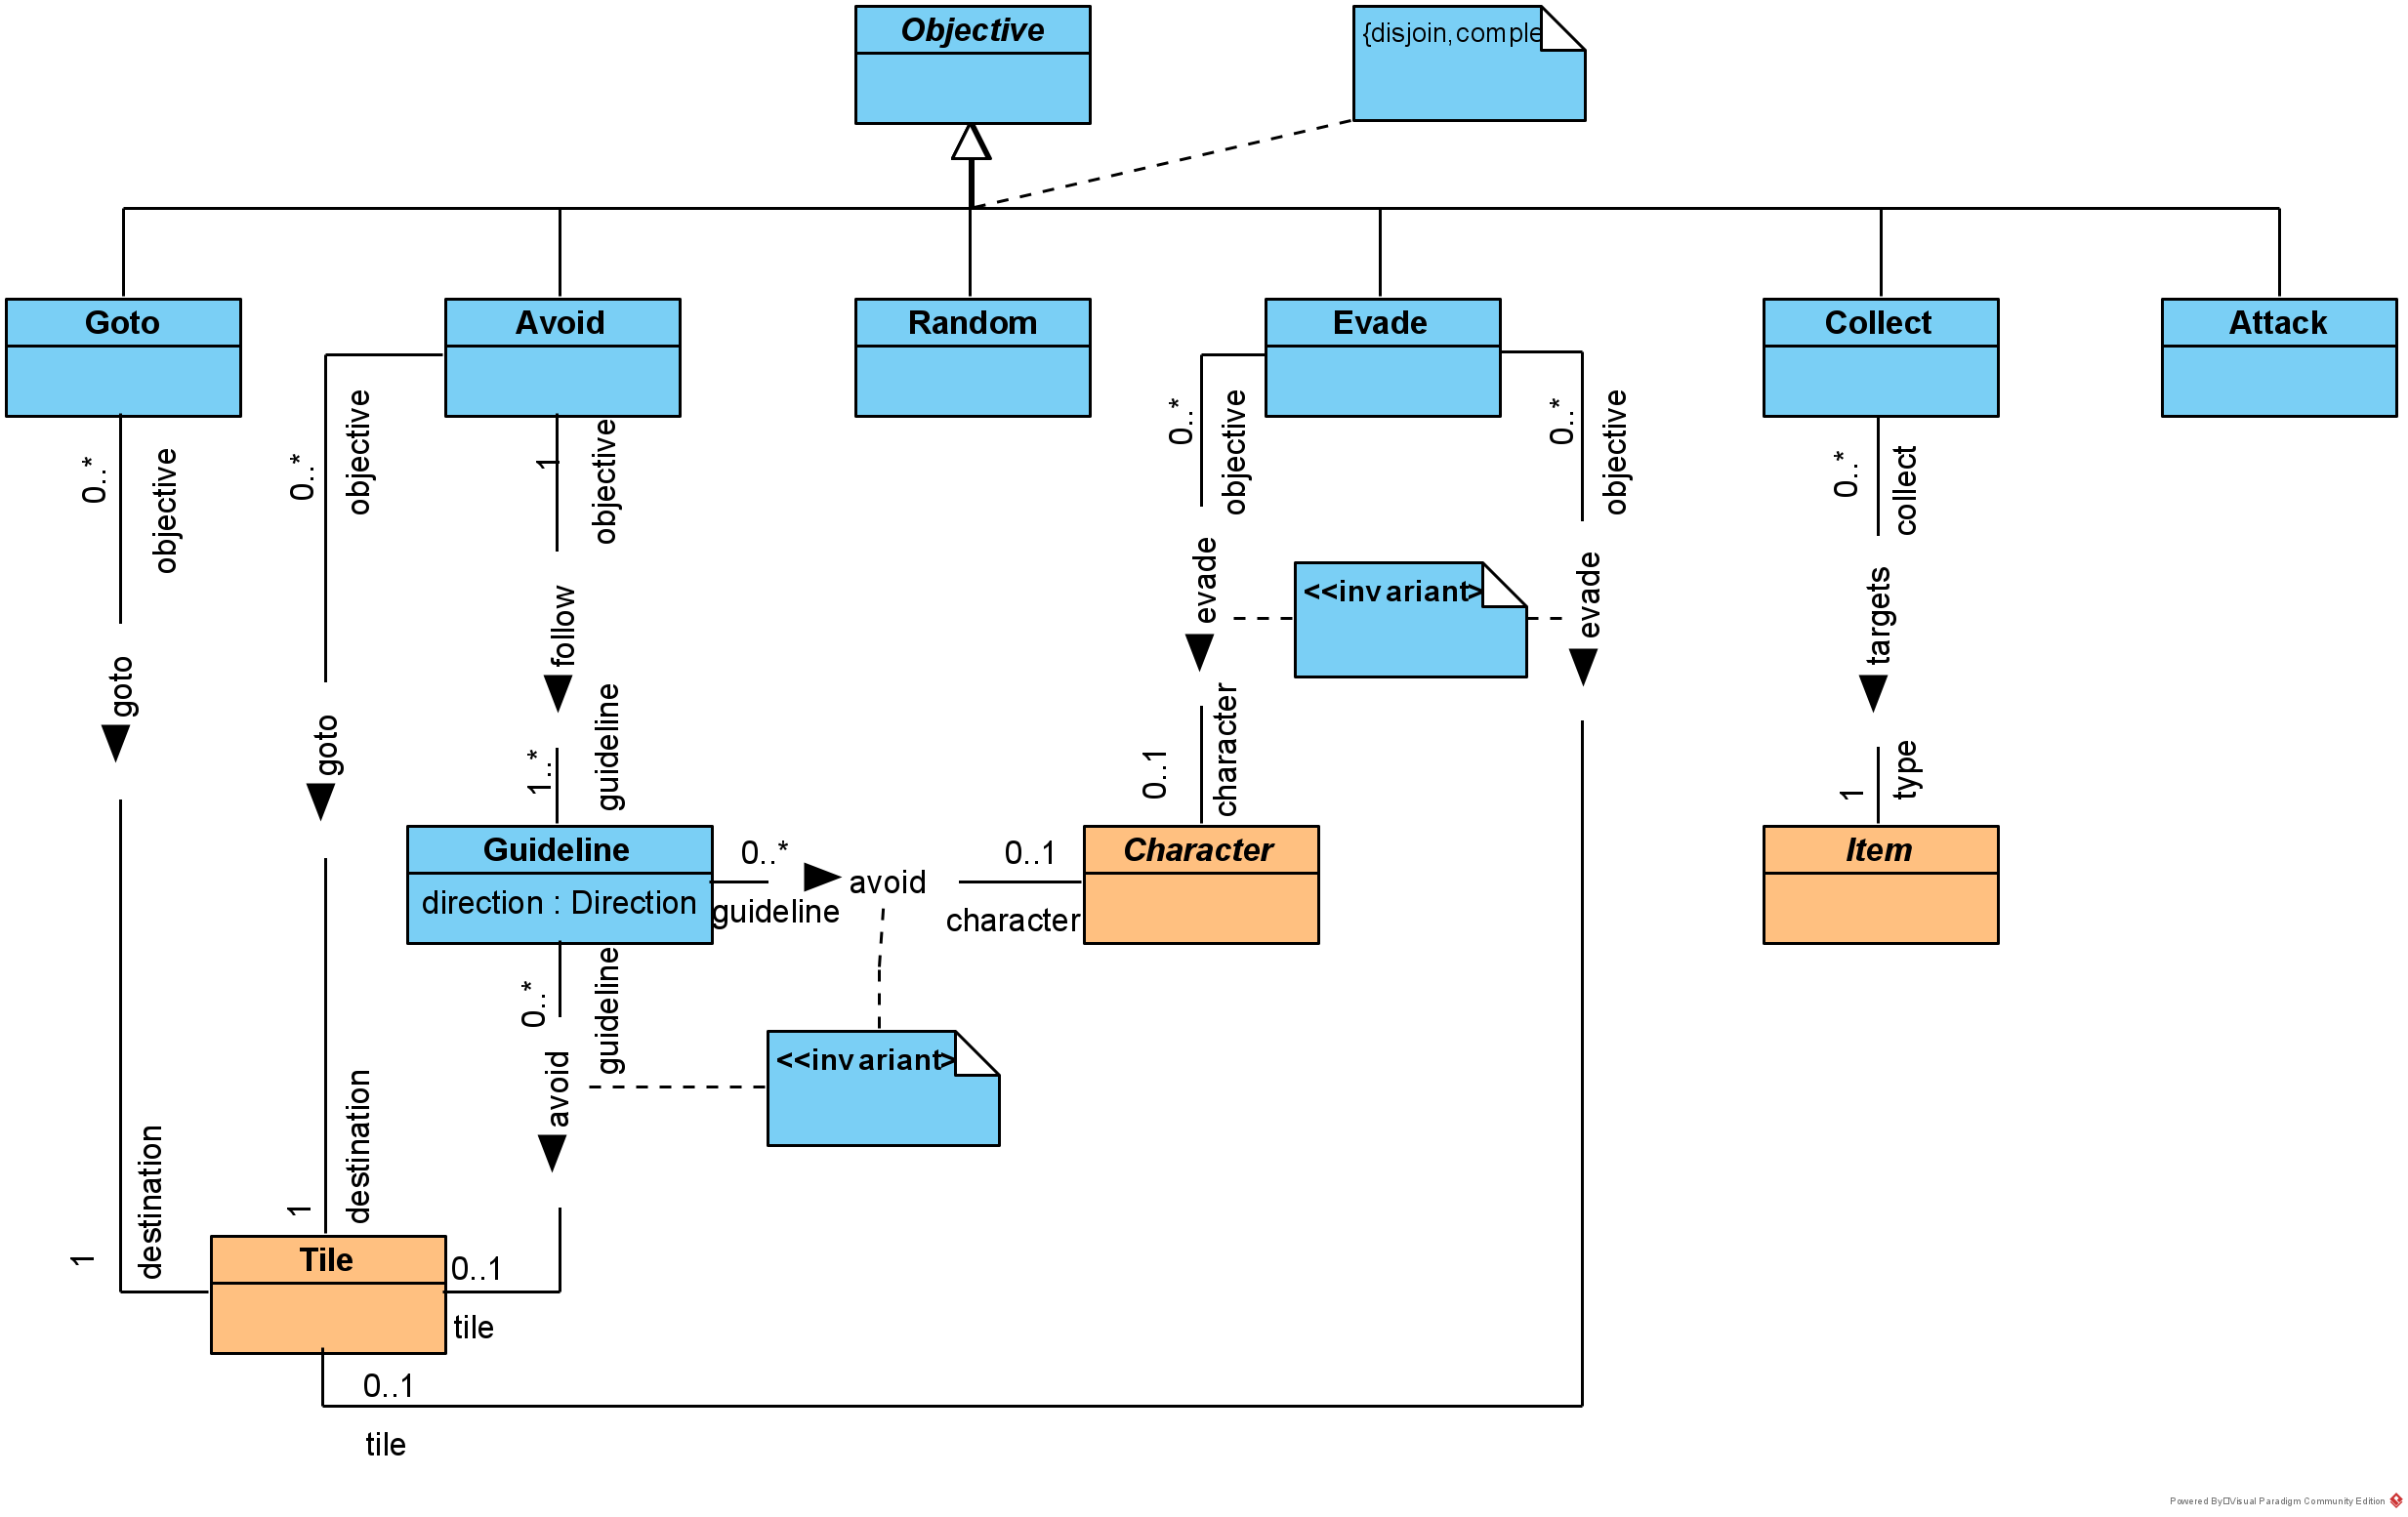
\includegraphics[width=\textwidth,height=\textheight,keepaspectratio]{Diagrams/DS-Objective.png}\newline

Les objectifs dirigent les comportements des personnages de la manière suivante :
\begin{itemize}
    \item L'objectif \textit{Néant} laisse le personnage errer de manière aléatoire et ne nécessite aucun paramètre.
    \item L'objectif \textit{AllerVers} donne à un personnage une case de destination et lui permet ainsi de déterminer à un chemin à suivre.
    \begin{tcolorbox}
        La spécification n'indique pas si l'objectif \textit{AllerVers} peut prendre un personnage plutôt qu'une case (comme pour la stratégie d'évitement). Nous avons donc choisi de ne pas représenter cette possibilité.
    \end{tcolorbox}
    \item L'objectif \textit{Contourner} donne à nouveau à un personnage une case du destination, mais également un ensemble de contraintes à respecter pour tracer son chemin jusqu'à cette case : un ensemble d'obstacles et/ou de personnages à éviter, ainsi que le côté cardinal par lequel les dépasser.
    \begin{tcolorbox}
        Les consignes de contournement prennent chacune en paramètre soit une case, soit un personnage (contrainte XOR).
    \end{tcolorbox}
    \item L'objectif \textit{Éviter} est le pendant inverse d'un objectif \textit{AllerVers} : le personnage reçoit à nouveau une case, mais celle-ci est cette fois-ci la case dont il faut s'éloigner. Le personnage peut donc à nouveau déterminer un chemin. 
    \begin{tcolorbox}
        Les consignes d'évitement peuvent prendre une case ou un joueur (au moins un et jamais deux) (contrainte XOR).
    \end{tcolorbox}
    \item L'objectif \textit{Combattre} ne prend pas de paramètre car il instruit au personnage non pas d'attaquer un ennemi en particulier, mais de choisir de lui-même selon une logique indéfinie les ennemis à attaquer : ennemi le plus proche, préséance de cible vers les autres joueurs plutôt que les zombies, etc.
    \item L'objectif \textit{CollecterMax} donne à l'avatar un exemple d'objet à ramasser autant que possible.
    \begin{tcolorbox}
        Cet objectif diffère des autres objectifs en ce sens qu'il fait appel au méta-modèle\,: plus qu'un objet, c'est une classe d'objet telle que décrite dans la description de jeu que cet objectif prend en compte. Nous avons cependant choisi de procéder de manière assez pragmatique en donnant un \textit{exemple} d'objet à ramaser plutôt qu'une abstraction issue du modèle.
    \end{tcolorbox}
\end{itemize}

Les objectifs sont dans une logique de spécialisation \textbf{disjointe} et \textbf{complète} : un objectif est nécessairement d'un et un seul sous-type. Le personnage peut cependant combiner deux objectifs grâce à la stratégie qui accepte un objectif de court terme et de long terme.\newline

\begin{samepage}
Par souci de cohérence linguistique, nous avons traduit les types d'objectifs comme suit :
\begin{center}
\begin{tabular}{c|c}
      \textbf{Terme} & \textbf{Traduction} \\\hline\hline
      Néant & \textit{Random}\\
      AllerVers & \textit{Goto}\\
      Contourner & \textit{Avoid}\\
      Éviter & \textit{Evade}\\
      Combattre & \textit{Fight}\\
      CollecterMax & \textit{Collect}\\
\end{tabular}
\end{center}
\end{samepage}

Décrivons ici comment l'enchaînement d'objectif cumulé à leur priorité peut influencer leur comportement en prenant deux objectifs et en les réorganisant:
\begin{center}
    \begin{tabular}{p{2,7cm}|p{5cm}|p{5cm}}
        \textbf{Stratégie} & \textbf{Cas 1} & \textbf{Cas 2}\\\hline\hline
         \textbf{STO} &  Goto(tile) & Collect(Consumable)\\\hline
         \textbf{LTO} & Collect(Consumable) & Goto(Tile)\\\hline
         \textbf{Réalisation} & Le personnage tente de rejoindre une tuile et fera des détours si nécessaires pour collecter des objets consommables. & Le personnage se rend vers une tuile pour collecter les objets alentours une fois sur place.\\
          & (trajet avec détour) & (trajet direct)
    \end{tabular}
\end{center}

\subsubsection{Action}

\textbf{Question 4.11.}\label{Question 4.11.}\newline

\nopagebreak 

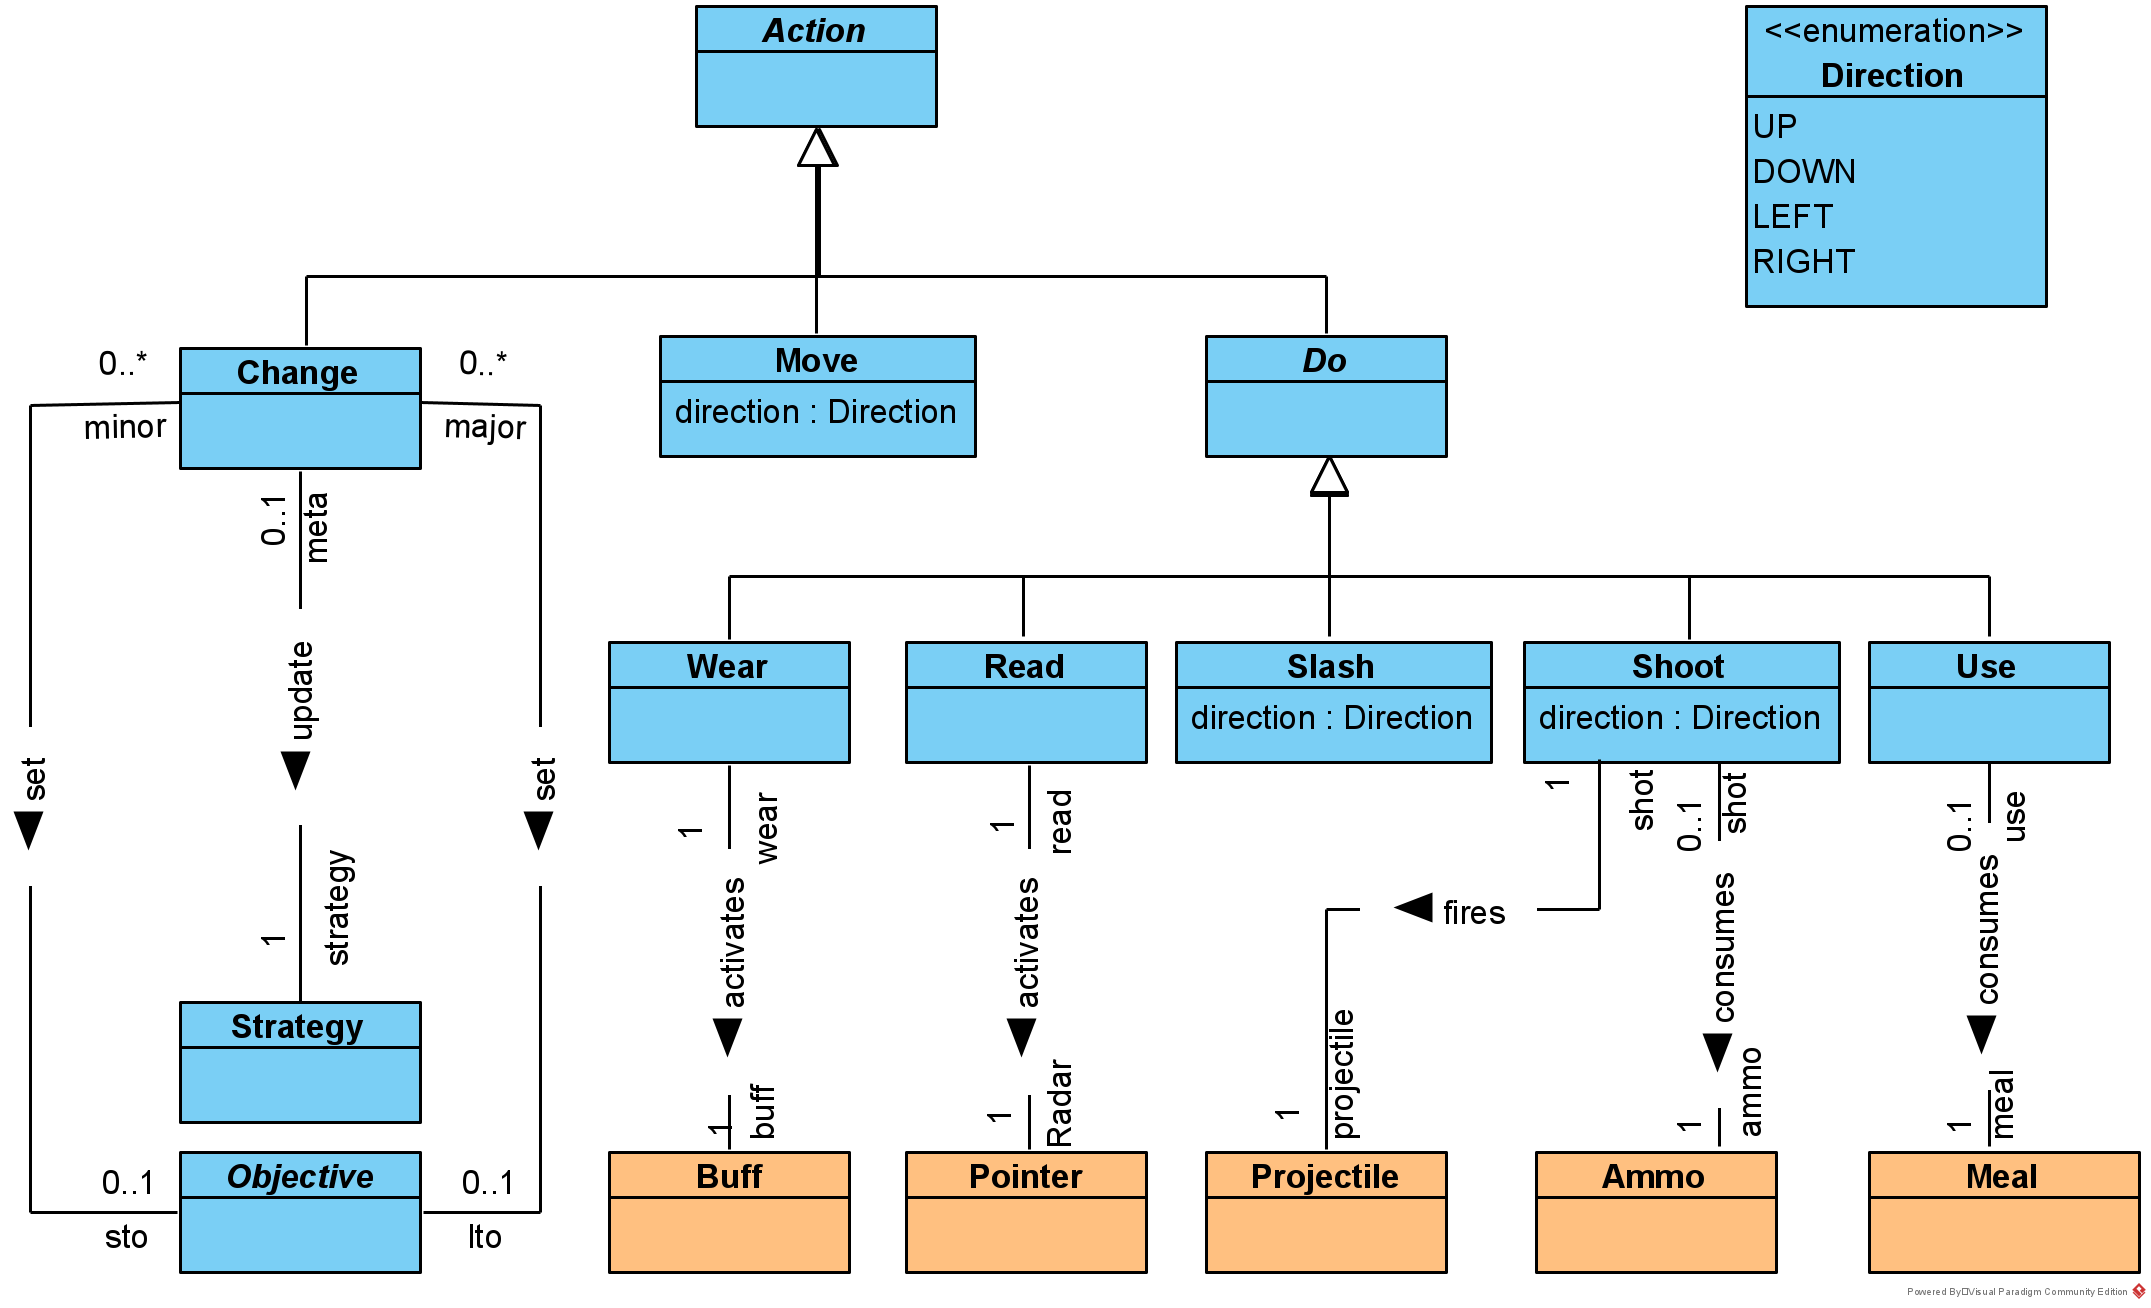
\includegraphics[width=\textwidth,height=\textheight,keepaspectratio]{Diagrams/DS-Action.png}

Les actions sont des types d'instruction spécifiques permettant au joueur de contrôler les actions de son personnage.
Elles se décomposent en trois catégories :
\begin{itemize}
    \item Les actions de type \textit{mouvement} (MOVE) permettent au personnage de se déplacer sur le plateau de jeu dans une des directions cardinales.
    \item Les actions de type \textit{activité} (DO) permettent au personnage d'interagir avec le monde qui l'entoure.
    \item Les actions de type \textit{méta} (META) permettent au joueur de provoquer un changement de comportement de leur personnage.
\end{itemize}

Par souci de cohérence linguistique, nous avons traduit les types d'activités comme suit :
\begin{center}
\begin{tabular}{c|c}
      \textbf{Terme} & \textbf{Traduction} \\\hline\hline
      Frapper & \textit{Slash}\\
      Tirer & \textit{Shoot}\\
      UtiliserItem & \textit{Use}\\
      Revêtir & \textit{Wear}\\
      ConsulterRadar & \textit{Read}\\
\end{tabular}
\end{center}

\begin{samepage}
Les actions nécessitent différents paramètres :
\begin{itemize}
    \item L'action \textit{Revêtir} nécessite logiquement d'avoir un objet enfilable (cape de mage ou cotte de maille).
    \item L'action \textit{Lire} nécessite tout aussi logiquement d'avoir un objet d'aide à l'orientation à disposition.
    \item L'action \textit{Frapper} ne prend pas de paramètre en entrée et consiste à faire tournoyer l'épée dans une certaine direction.
        \begin{tcolorbox}
            Nous aurions pu requérir que cette action nécessite d'avoir un ennemi ou un obstacle destructible en face. Cependant, il nous a semblé qu'un personnage pouvait jouer les Don Quichotte et de frapper dans le vide, sans cible, ou s'acharner à escrimer un mur infranchissable par frustration. 
        \end{tcolorbox}
    \item L'action \textit{Tirer} nécessite de pouvoir consommer une munition depuis l'inventaire et envoie alors un projectile dans la direction demandée.
    \item L'action \textit{UtiliserItem} permet enfin de regagner quelques points de vie en mangeant un repas bien mérité (càd nourriture et boisson).
\end{itemize}
\end{samepage}

\subsection{Langage}

\subsubsection{Déclaration}
\textbf{Question 4.9.}\label{Question 4.9.}\newline

\nopagebreak 

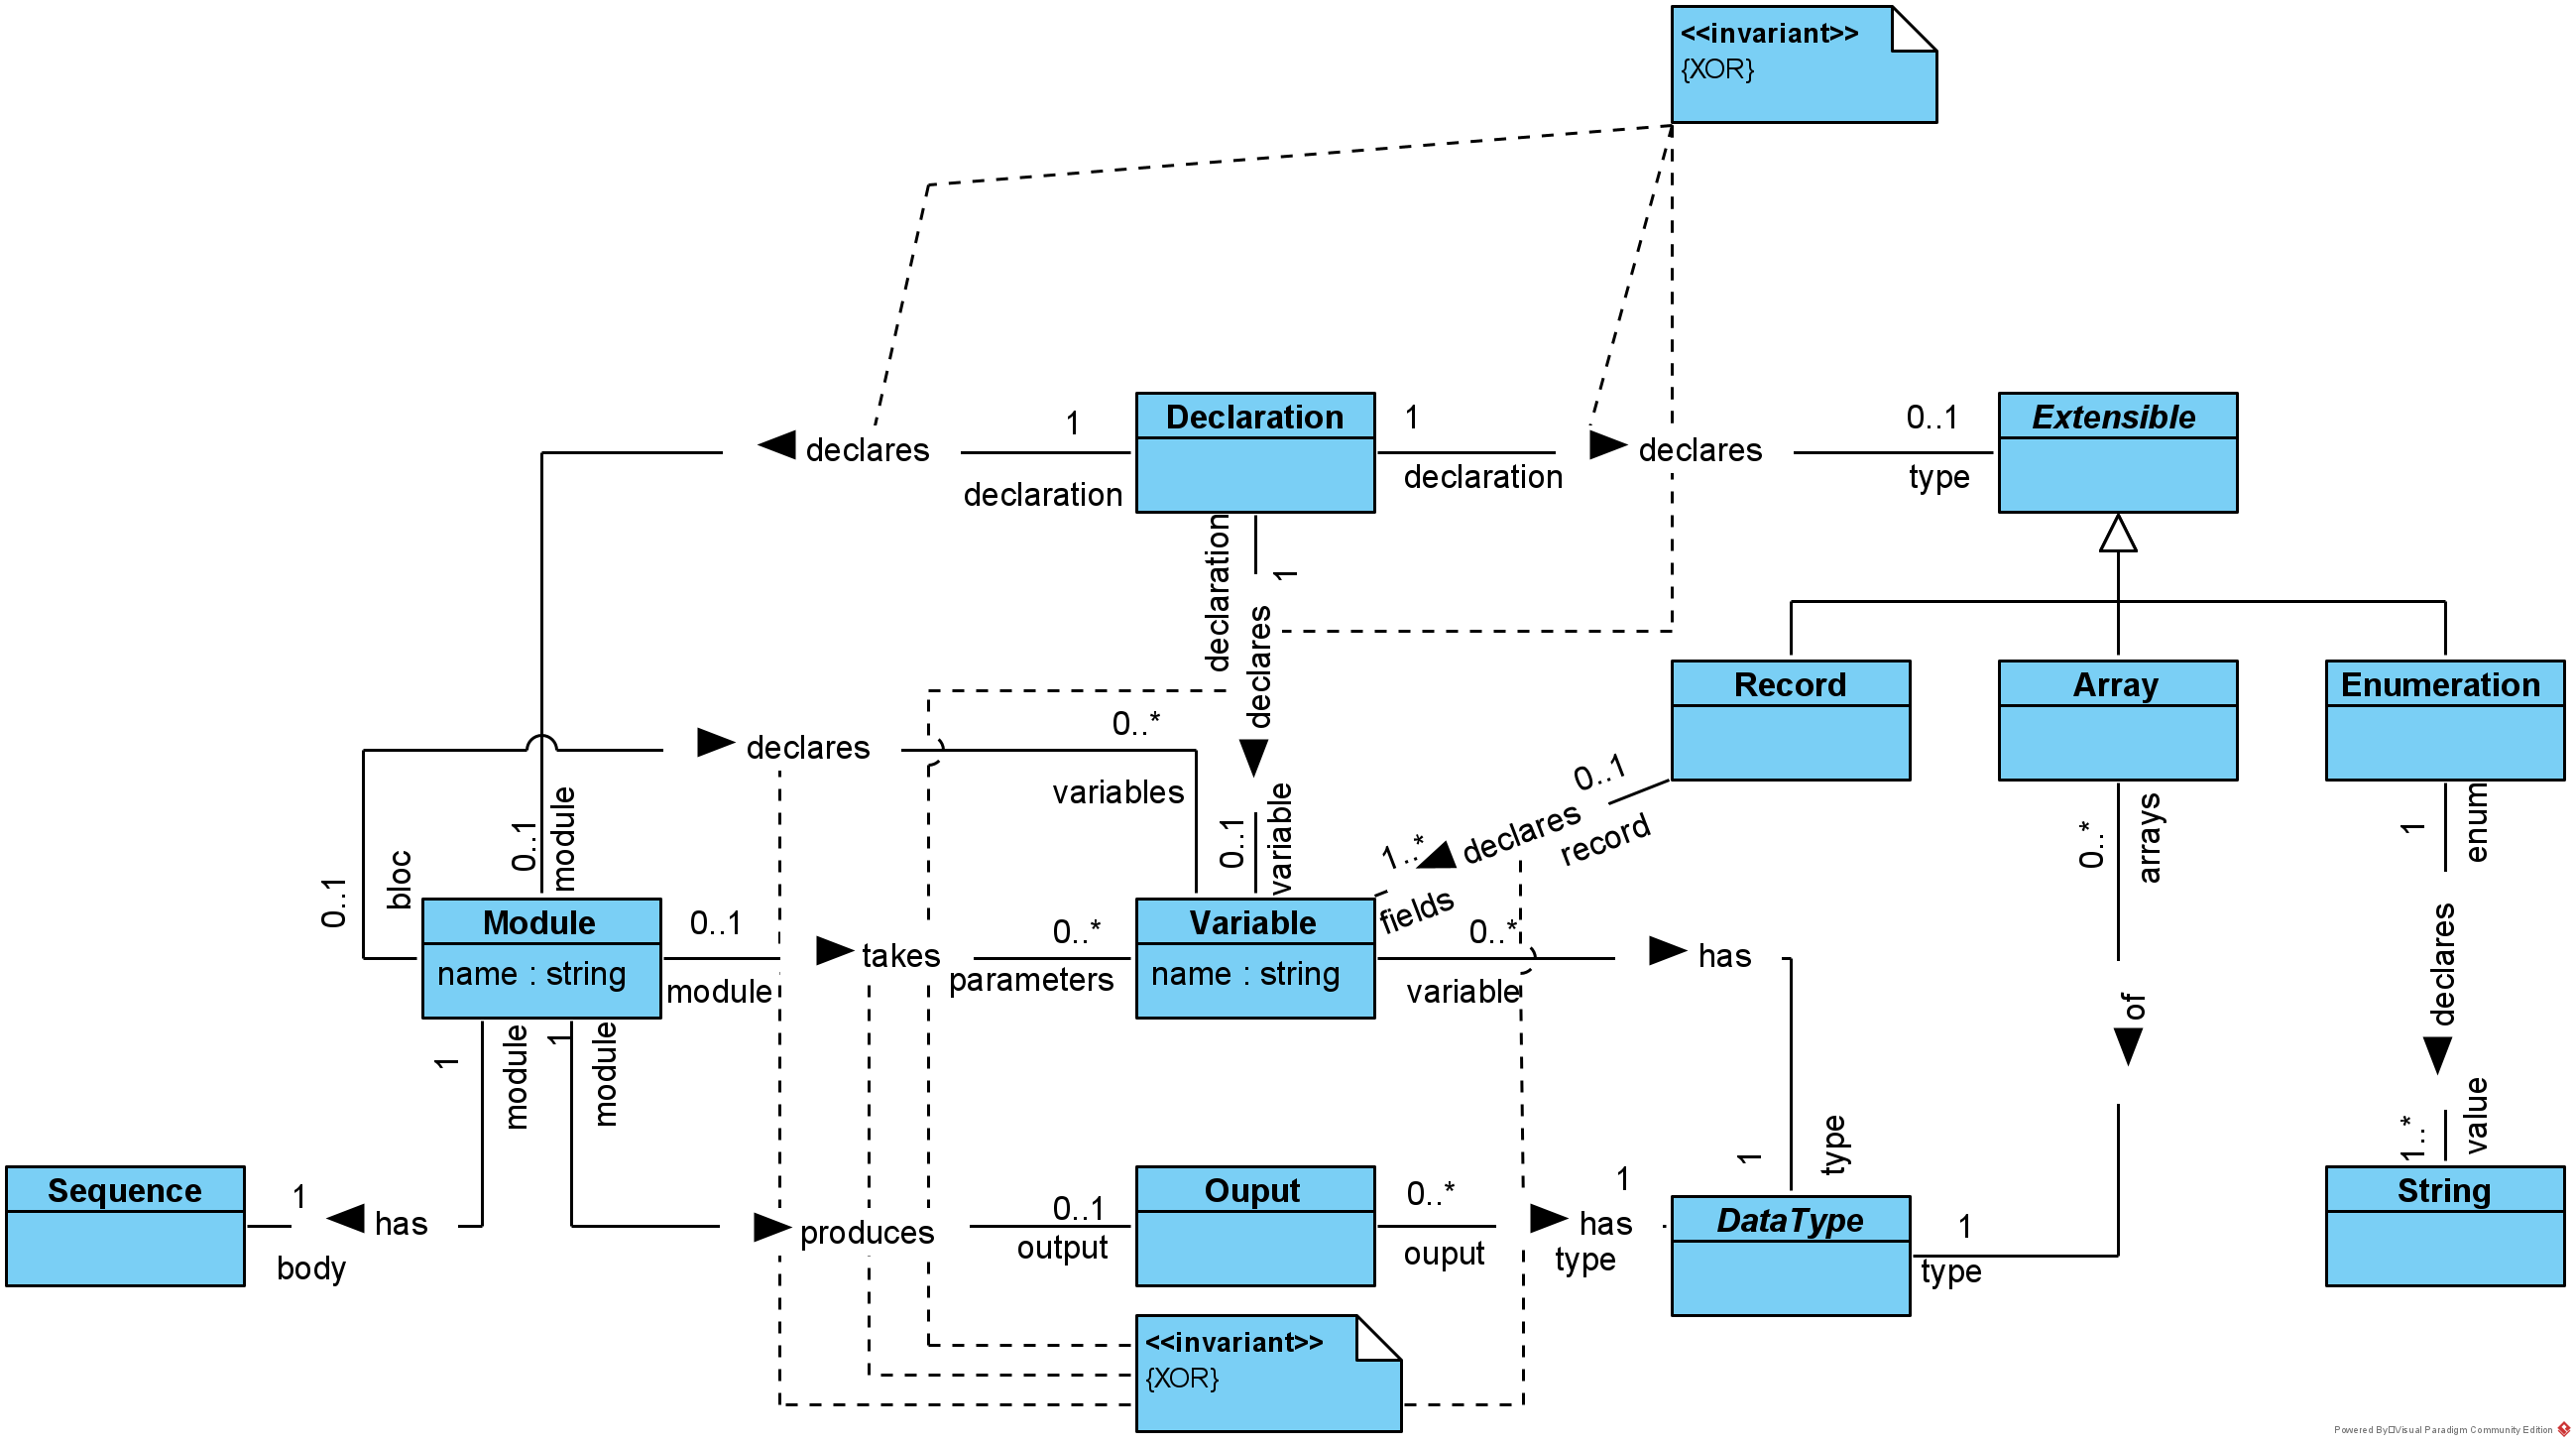
\includegraphics[width=\textwidth,height=\textheight,keepaspectratio]{Diagrams/DS-Declaration.png}\newline

Nous avons dénombré trois types distincts de déclarations :
\begin{itemize}
    \item Les déclarations de modules ;
    \item Les déclarations de variables ;
    \item Les déclarations de types extensibles (tableau, enregistrement, énumération).
\end{itemize}\newline

\lstset{
	tabsize=4,
	rulecolor=,
    emph={total, shortestDistance, start, stop, x, y},emphstyle={\color{dark-green}},
    basicstyle=\footnotesize\ttfamily,
    upquote=true,
    aboveskip={1.5\baselineskip},
    columns=fixed,
    showstringspaces=false,
    extendedchars=true,
    breaklines=true,
    prebreak = \raisebox{0ex}[0ex][0ex]{\ensuremath{\hookleftarrow}},
    frame=none,
    showtabs=false,
    showspaces=false,
    showstringspaces=false,
    stringstyle=\color{pred},
    keywords={var, module, type},
    keywordstyle=\slshape\bfseries,
    classoffset=1,
    keywordstyle={\color[rgb]{0,0,1}\bfseries},
    morekeywords={boolean},
    classoffset=0,
    commentstyle=\color[rgb]{0.133,0.545,0.133},
    stringstyle=\color[rgb]{0.627,0.126,0.941},
}
\begin{minipage}[t]{.33\textwidth}
    \textit{Variables}
     \begin{lstlisting}
var total : integer;
     \end{lstlisting}
\end{minipage}
\begin{minipage}[t]{.33\textwidth}
    \textit{Modules}
     \begin{lstlisting}
module shortestDistance
param start, stop : Cell
produces integer
begin
var count : integer
...
end
     \end{lstlisting}
\end{minipage}
\begin{minipage}[t]{.33\textwidth}
    \textit{Types extensibles}
     \begin{lstlisting}
type Cell : record
    x : integer;
    y : integer;
endrecord

type Sight = array[1..MAX] of integer;

type majuscule = 'A'..'Z';
     \end{lstlisting}
\end{minipage}\newline

\begin{samepage}
Une variable est simplement une entité-mémoire nommée et associée à un type de données. Elles sont présentes à plusieurs niveaux dans le langage de programmation des stratégies :
    \begin{itemize}
        \item En tant qu'objet explicitement déclaré.
        \item en tant que paramètre d'un module
        \item en tant que champ d'un enregistrement.
    \end{itemize}
\end{samepage}

Un module est quant à lui un objet plus complexe, qui encapsule une logique de programmation. Il possède lui aussi un nom et déclare lui-même une série de paramètres et une valeur de retour si nécessaire. Il possède en outre un corps d'instructions permettant de réaliser effectivement sa logique.  Outre ses paramètres, le module peut également faire ses propres déclarations internes (de variables uniquement\newline

Enfin, un type extensible n'existe pas en tant que tel dans le langage : ils doivent nécessairement avoir été déclarés et définis à un moment ou l'autre dans le développement.
\begin{itemize}
    \item Un enregistrement doit avoir été nommé et la liste de ses champs doit avoir été explicitée (nom et type).
    \item Un tableau doit avoir été nommé, typé et dimensionné.
    \item Une énumération doit avoir été nommée, et ses valeurs énoncées.
\end{itemize}

\subsubsection{Type de données}

\textbf{Question 4.8.}\label{Question 4.8.}\newline
\nopagebreak 
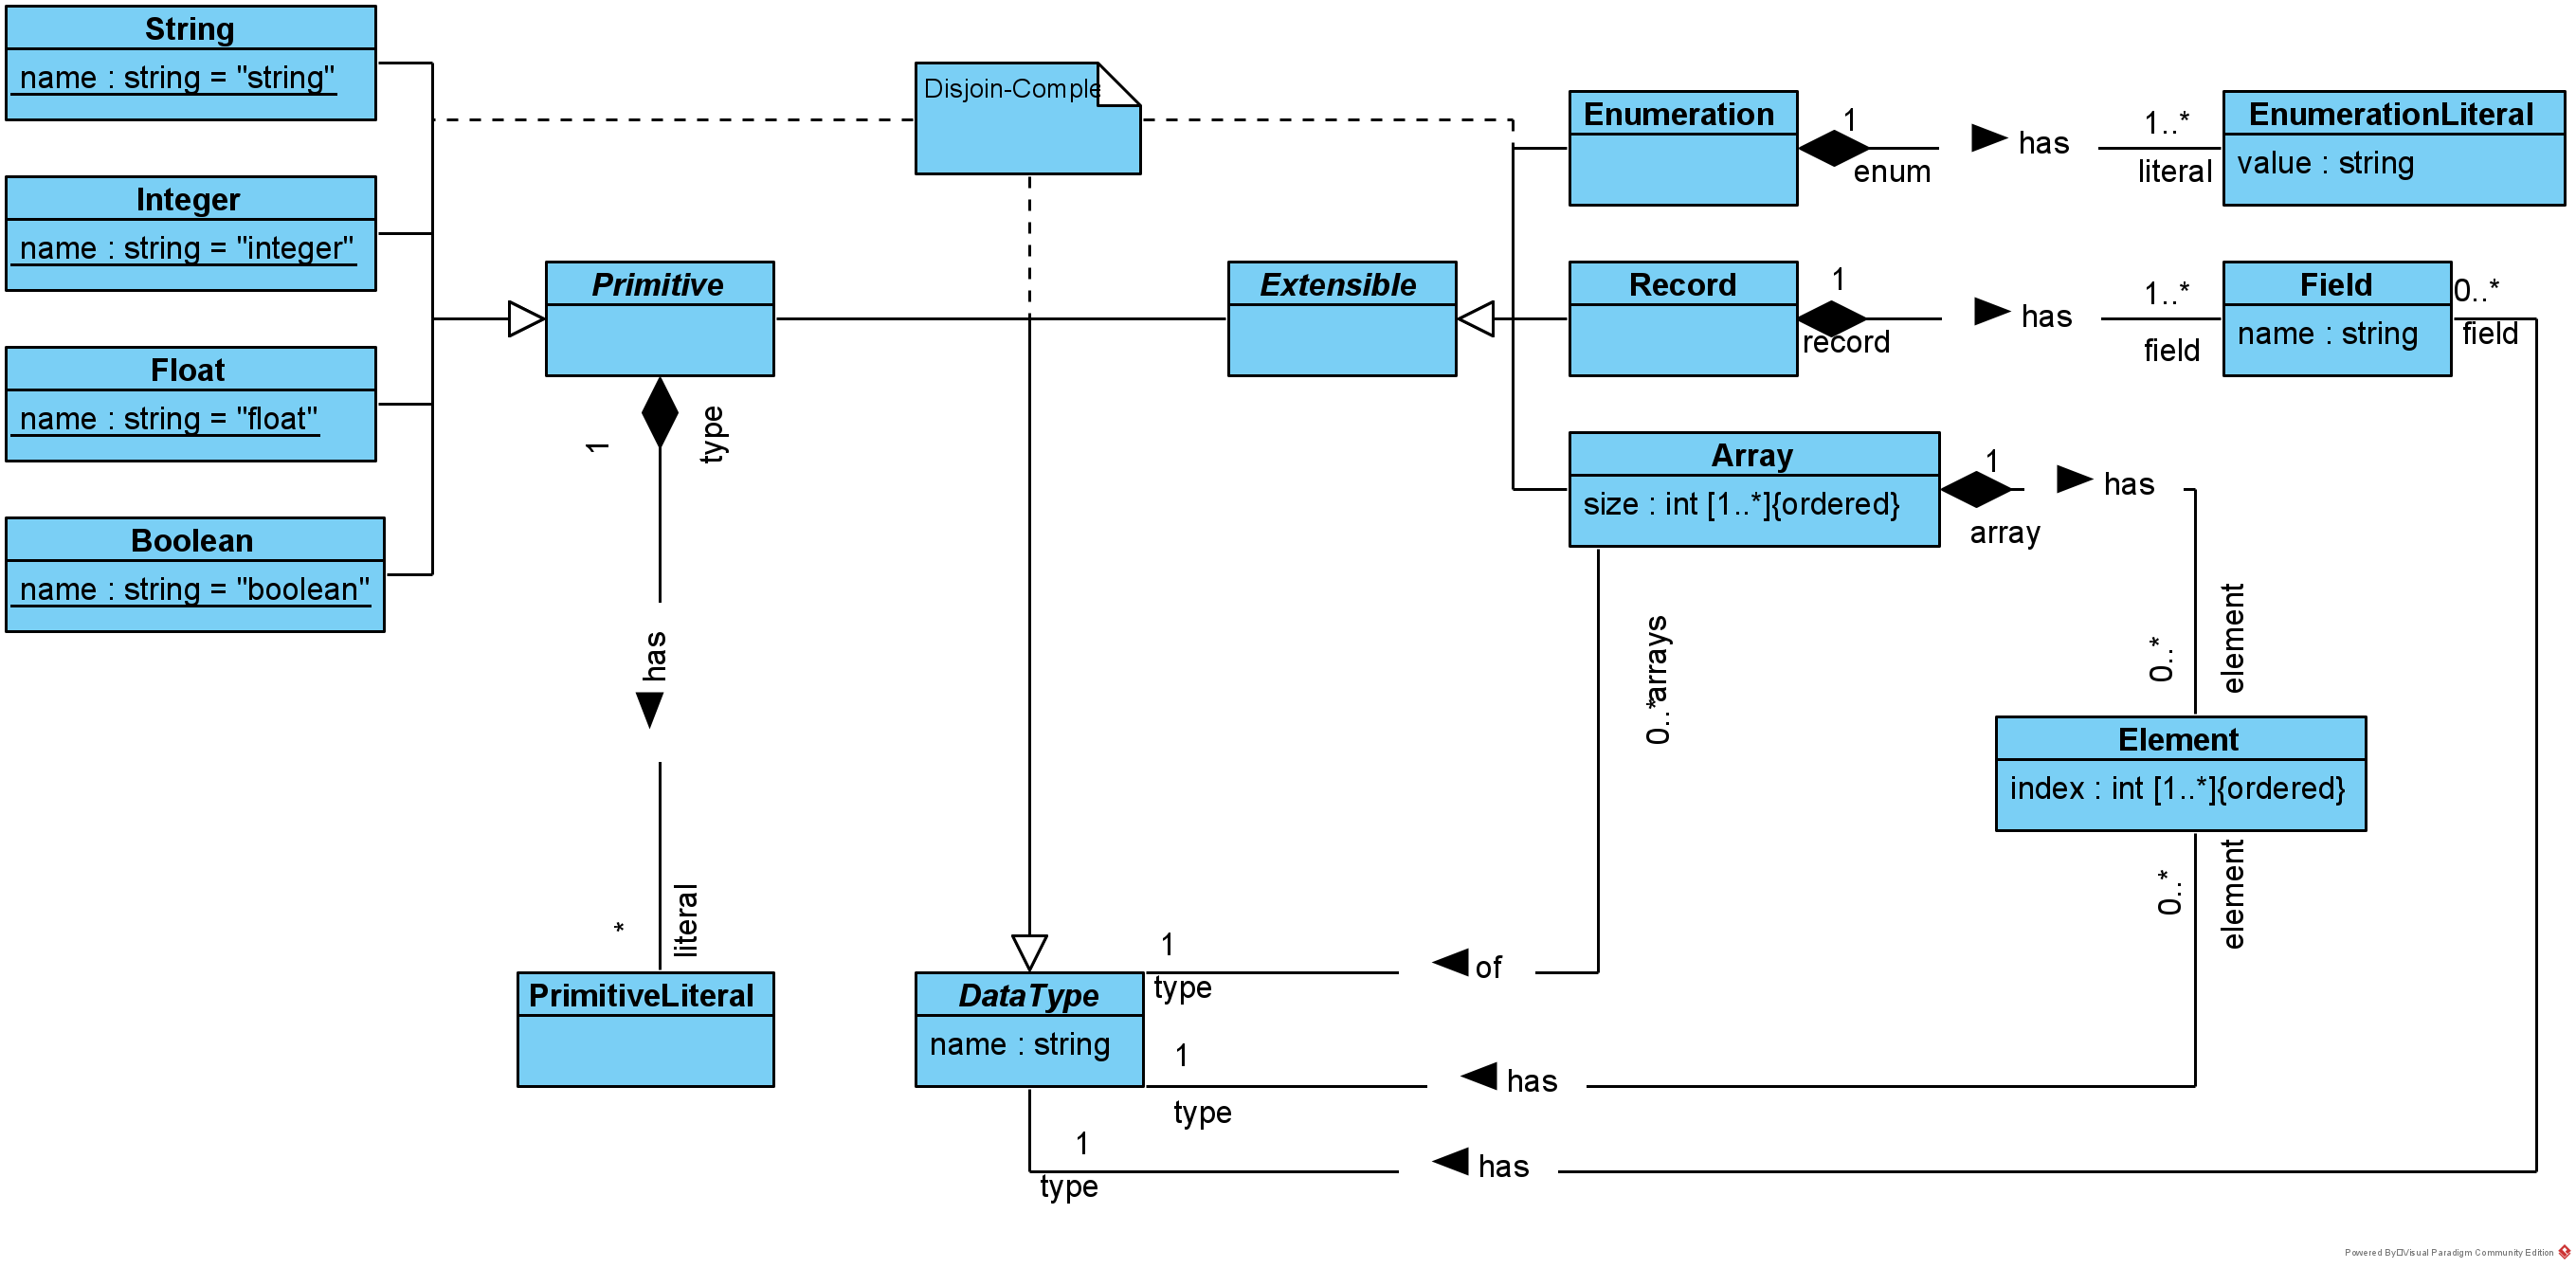
\includegraphics[width=\textwidth,height=\textheight,keepaspectratio]{Diagrams/DS-DataType.png}\newline

\begin{samepage}
    Les types de données peuvent être divisés en deux catégories :
    \begin{itemize}
        \item D'une part, les types \textit{"finis"} qui sont déclarés d'entrée de jeu de manière absolue et définitive\,: 
        \begin{itemize}
            \item types primitifs (entiers, décimaux, booléens, chaînes de caractères)
        \end{itemize}
        \item D'autre part, les types \textit{"extensibles"}, qui peuvent être ajoutés par les développeurs : 
        \begin{itemize}
            \item tableaux
            \item enregistrements
            \item énumérations
        \end{itemize} 
    \end{itemize}
\end{samepage}

Tout type de données est ensuite associé à un ensemble de valeurs possibles.
\begin{itemize}
    \item Les valeurs des types primitifs et des énumérations sont \textit{immédiates}, car leur signification n'est pas sujette à interprétation (ils n'ont qu'une seule valeur et celle-ci est exprimée directement).
    \item Les valeurs des types tableau et enregistrement ne sont en revanche pas aussi claires, ceux-ci étant avant tout des entités d'agrégation de données. Par récursion, ces types finissent toujours par être associés à des valeurs primitives ou des énumérations et peuvent ainsi recevoir une valeur \textit{immédiate}.
\end{itemize}

\subsubsection{Expression}

\textbf{Question 4.12.}\label{Question 4.12.}\newline

\nopagebreak 

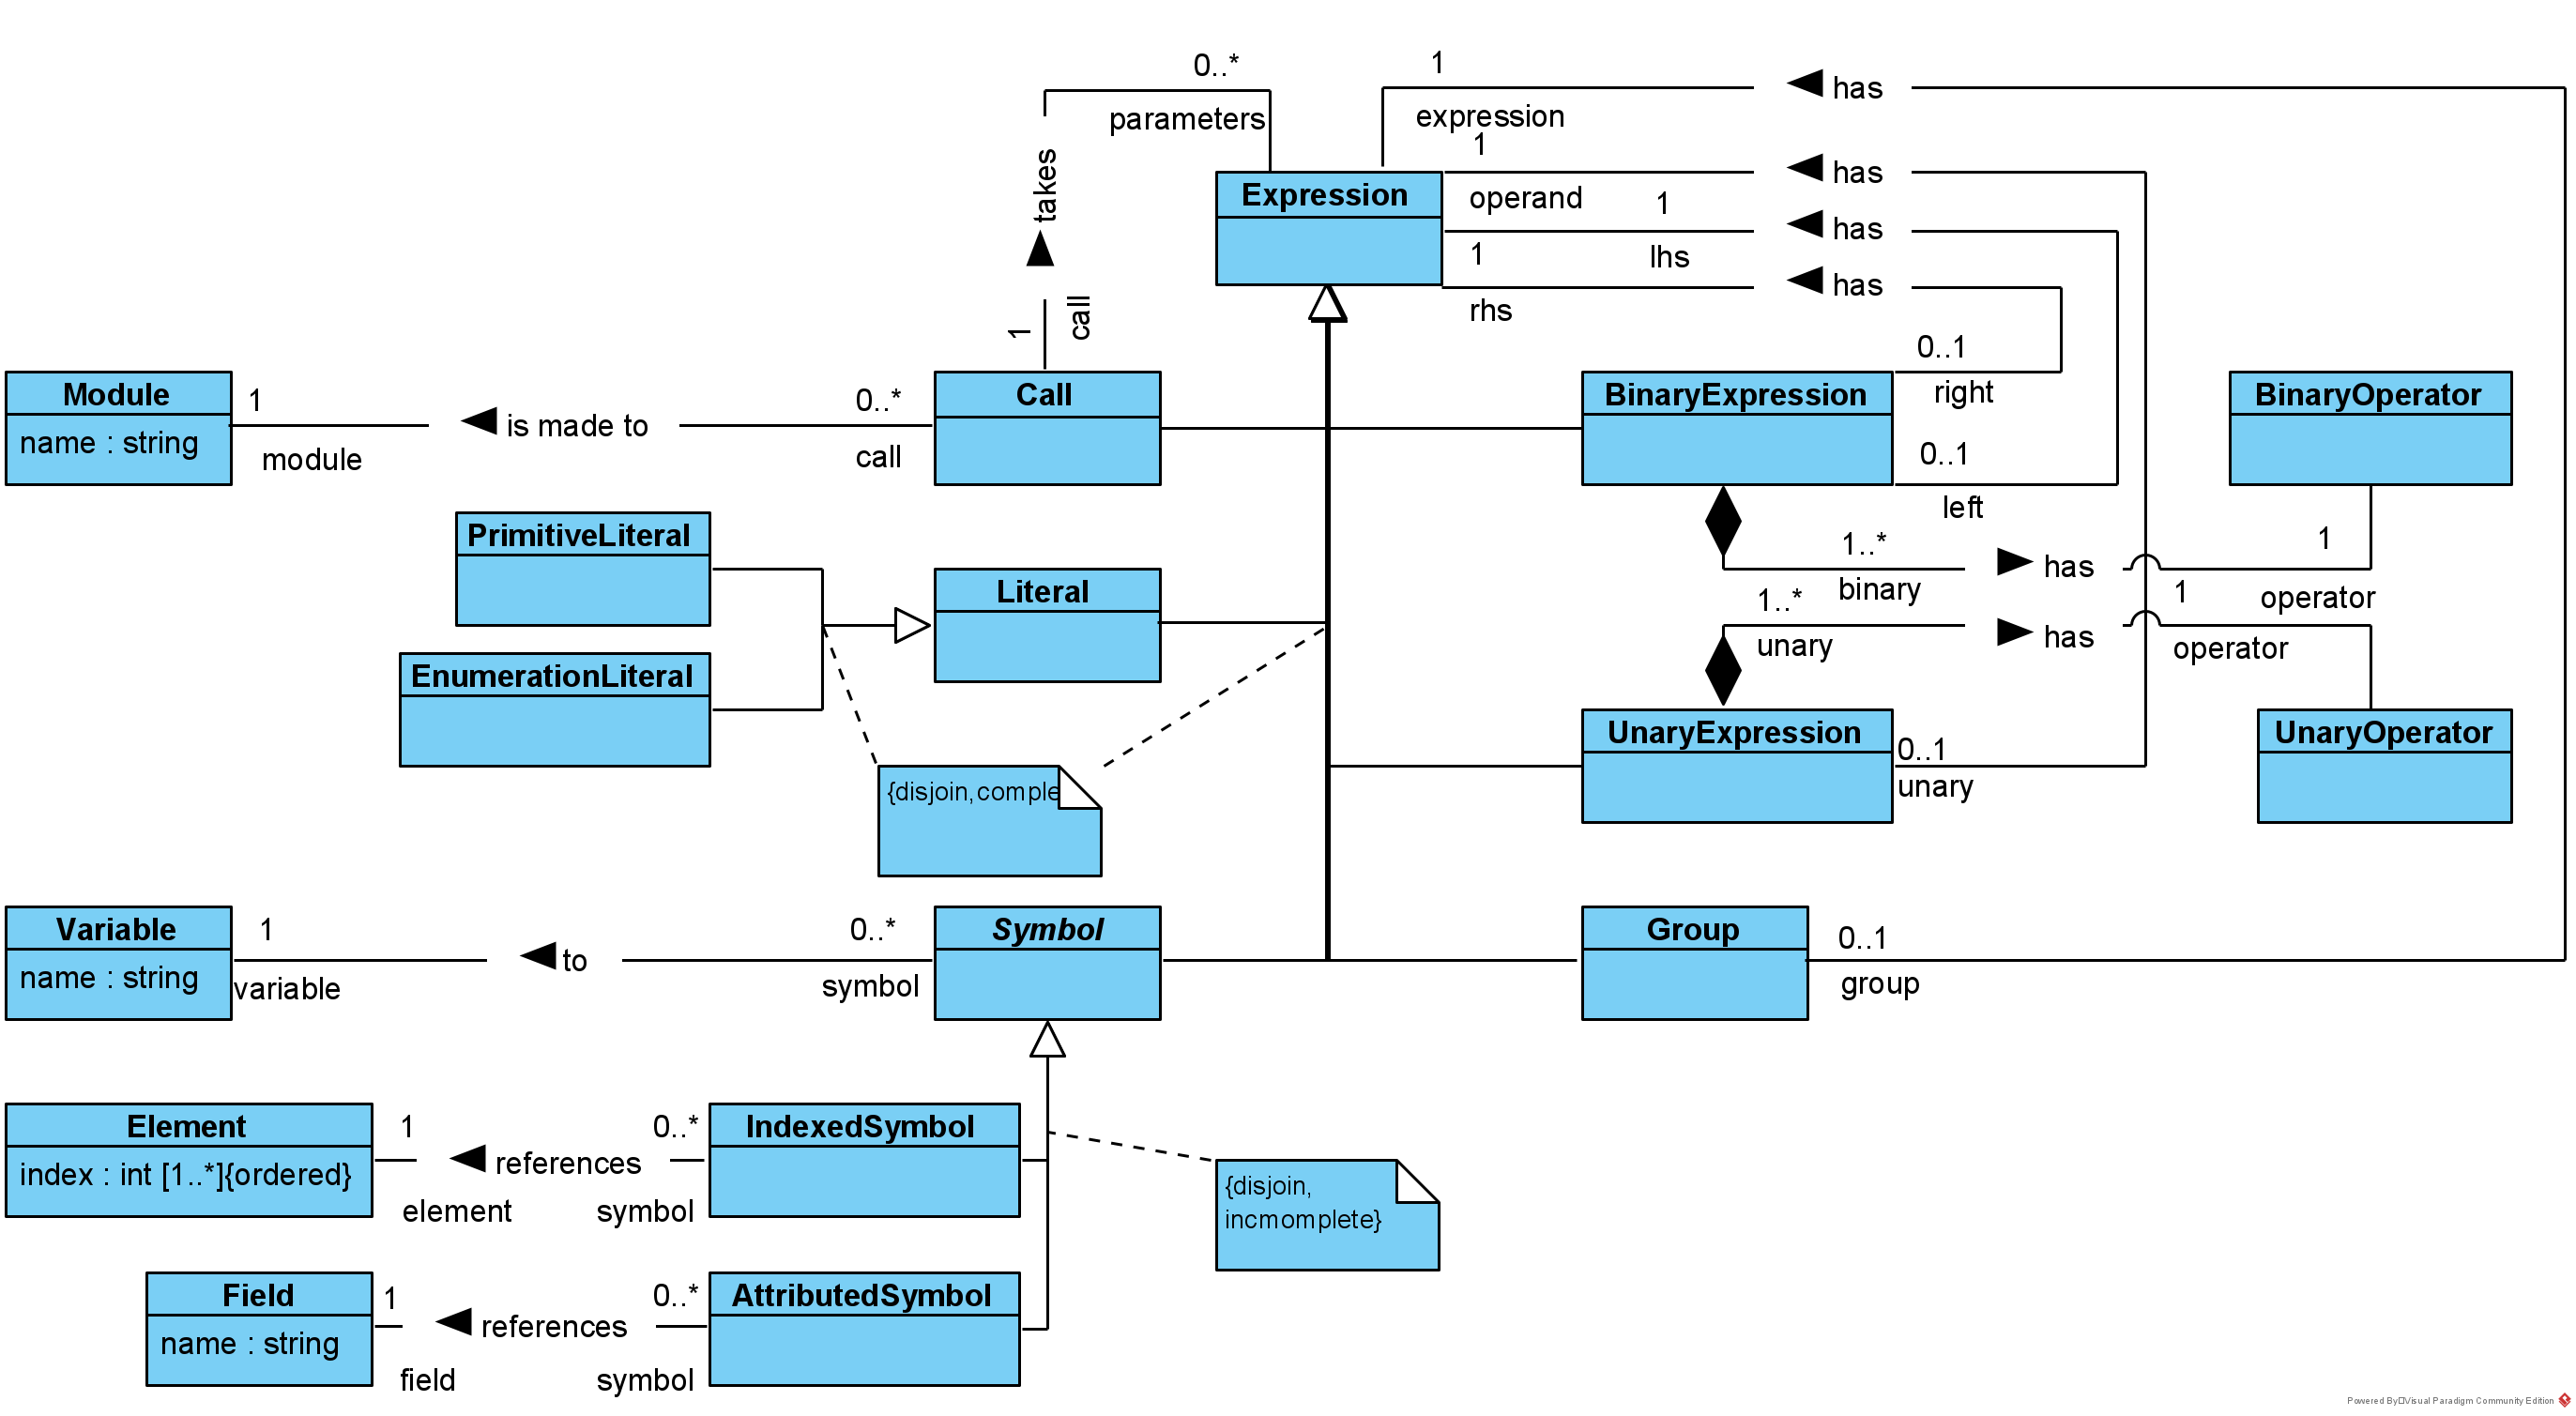
\includegraphics[width=\textwidth,height=\textheight,keepaspectratio]{Diagrams/DS-Expression.png}\newline

Nous pouvons distinguer les expressions sous trois catégories :
\begin{itemize}
    \item Les regroupements : expressions unaires, binaires et regroupées.
    \item Les appels : une expression structurée faisant appel à une séquence d'instruction.
    \item Les représentations : littéraux et symboles (tableaux, enregistrement, etc.).
\end{itemize}

Les expressions de \textbf{regroupement} sont marquées par une certaine forme de récursivité : elles peuvent être enchaînées de manière illimitée pour construire des expressions plus ou moins complexes et combiner des valeurs entre elles. Nous avons remarqué, pour les opérations unaires et binaires, la fonction structurelle des opérateurs : c'est la présence même de ces opérateurs qui constitue l'expression.\newline

Les \textbf{appels de module} font également preuve d'une certaine récursivité, puisqu'ils acceptent des expressions comme des valeurs comme paramètres. Ils font appel à un et un seul module.\newline

\begin{samepage}
Les \textbf{représentations} sont la partie la plus complexe de ce diagramme : nous les avons réparties en deux groupes :
\begin{itemize}
    \item Les valeurs \textit{litérales}, dont le sens est immédiatement perceptible (comme précisé dans la spécification de ce projet et rappelé au point Datatype).
    \item Les valeurs \textit{interprétables}, dont il faut évaluer la référence.
\end{itemize}
\end{samepage}

Les valeurs littérales font directement référence aux valeurs qui sont associées aux types primitifs et aux énumérations : il y a une bijection entre l'ensemble des valeurs concrètes et celui de leur représentation littérale dans les expressions. A l'inverse, les éléments symbolisés (\textit{LHS} dans la spécification) sont des éléments qui peuvent représenter une même information d'autant de manières qu'il y a de déclarations. Nous avons cependant à nouveau distingué trois catégories :
\begin{itemize}
    \item Les symboles \textit{purs} font directement référence à une entrée en mémoire par le nom qui lui a été assigné au cours d'une déclaration. 
    \item Les symboles \textit{indicés} font référence à un élément au sein d'une entrée en mémoire groupée et arrangée (tableau). Dans ce cas, le symbole fait référence à la variable de regroupement et indique ensuite l'emplacement de la valeur à récupérer.
    \item Les symboles \textit{attribués} font référence à un élément au sein d'une entrée-mémoire structurée (enregistrement). Dans ce cas, le symbole fait référence par la variable à la structure générale et indique ensuite le nom de la valeur à récupérer au sein de cette structure.
\end{itemize}

\begin{tcolorbox}
    La modélisation que nous avons choisi ici ne permet pas de gérer l'imbrication de symboles. Par exemple, il n'admettrait pas un symbole tel que monTableau[1].monChamp. Pour pouvoir traiter ce cas, notre modèle nécessite de passer par plusieurs opérations d'assignation successives : 
    \begin{itemize}
        \item Récupérer l'enregistrement dans une variable intermédiaire.
        \item Récupérer le champ souhaité depuis la variable intermédiaire.
    \end{itemize}
        \begin{lstlisting}
                var monEnregistrement : Record = monTableau[1];
                var monChamp : string = monEnregistrement.monChamp;
        \end{lstlisting}
\end{tcolorbox}

Pour les symboles, nous avons choisi d'utiliser une relation de spécialisation disjointe, mais pas complète : un symbole n'est en effet pas forcément indicé ou attribué.

\subsubsection{Instruction}

\textbf{Question 4.13.}\label{Question 4.13.}\newline

\nopagebreak 

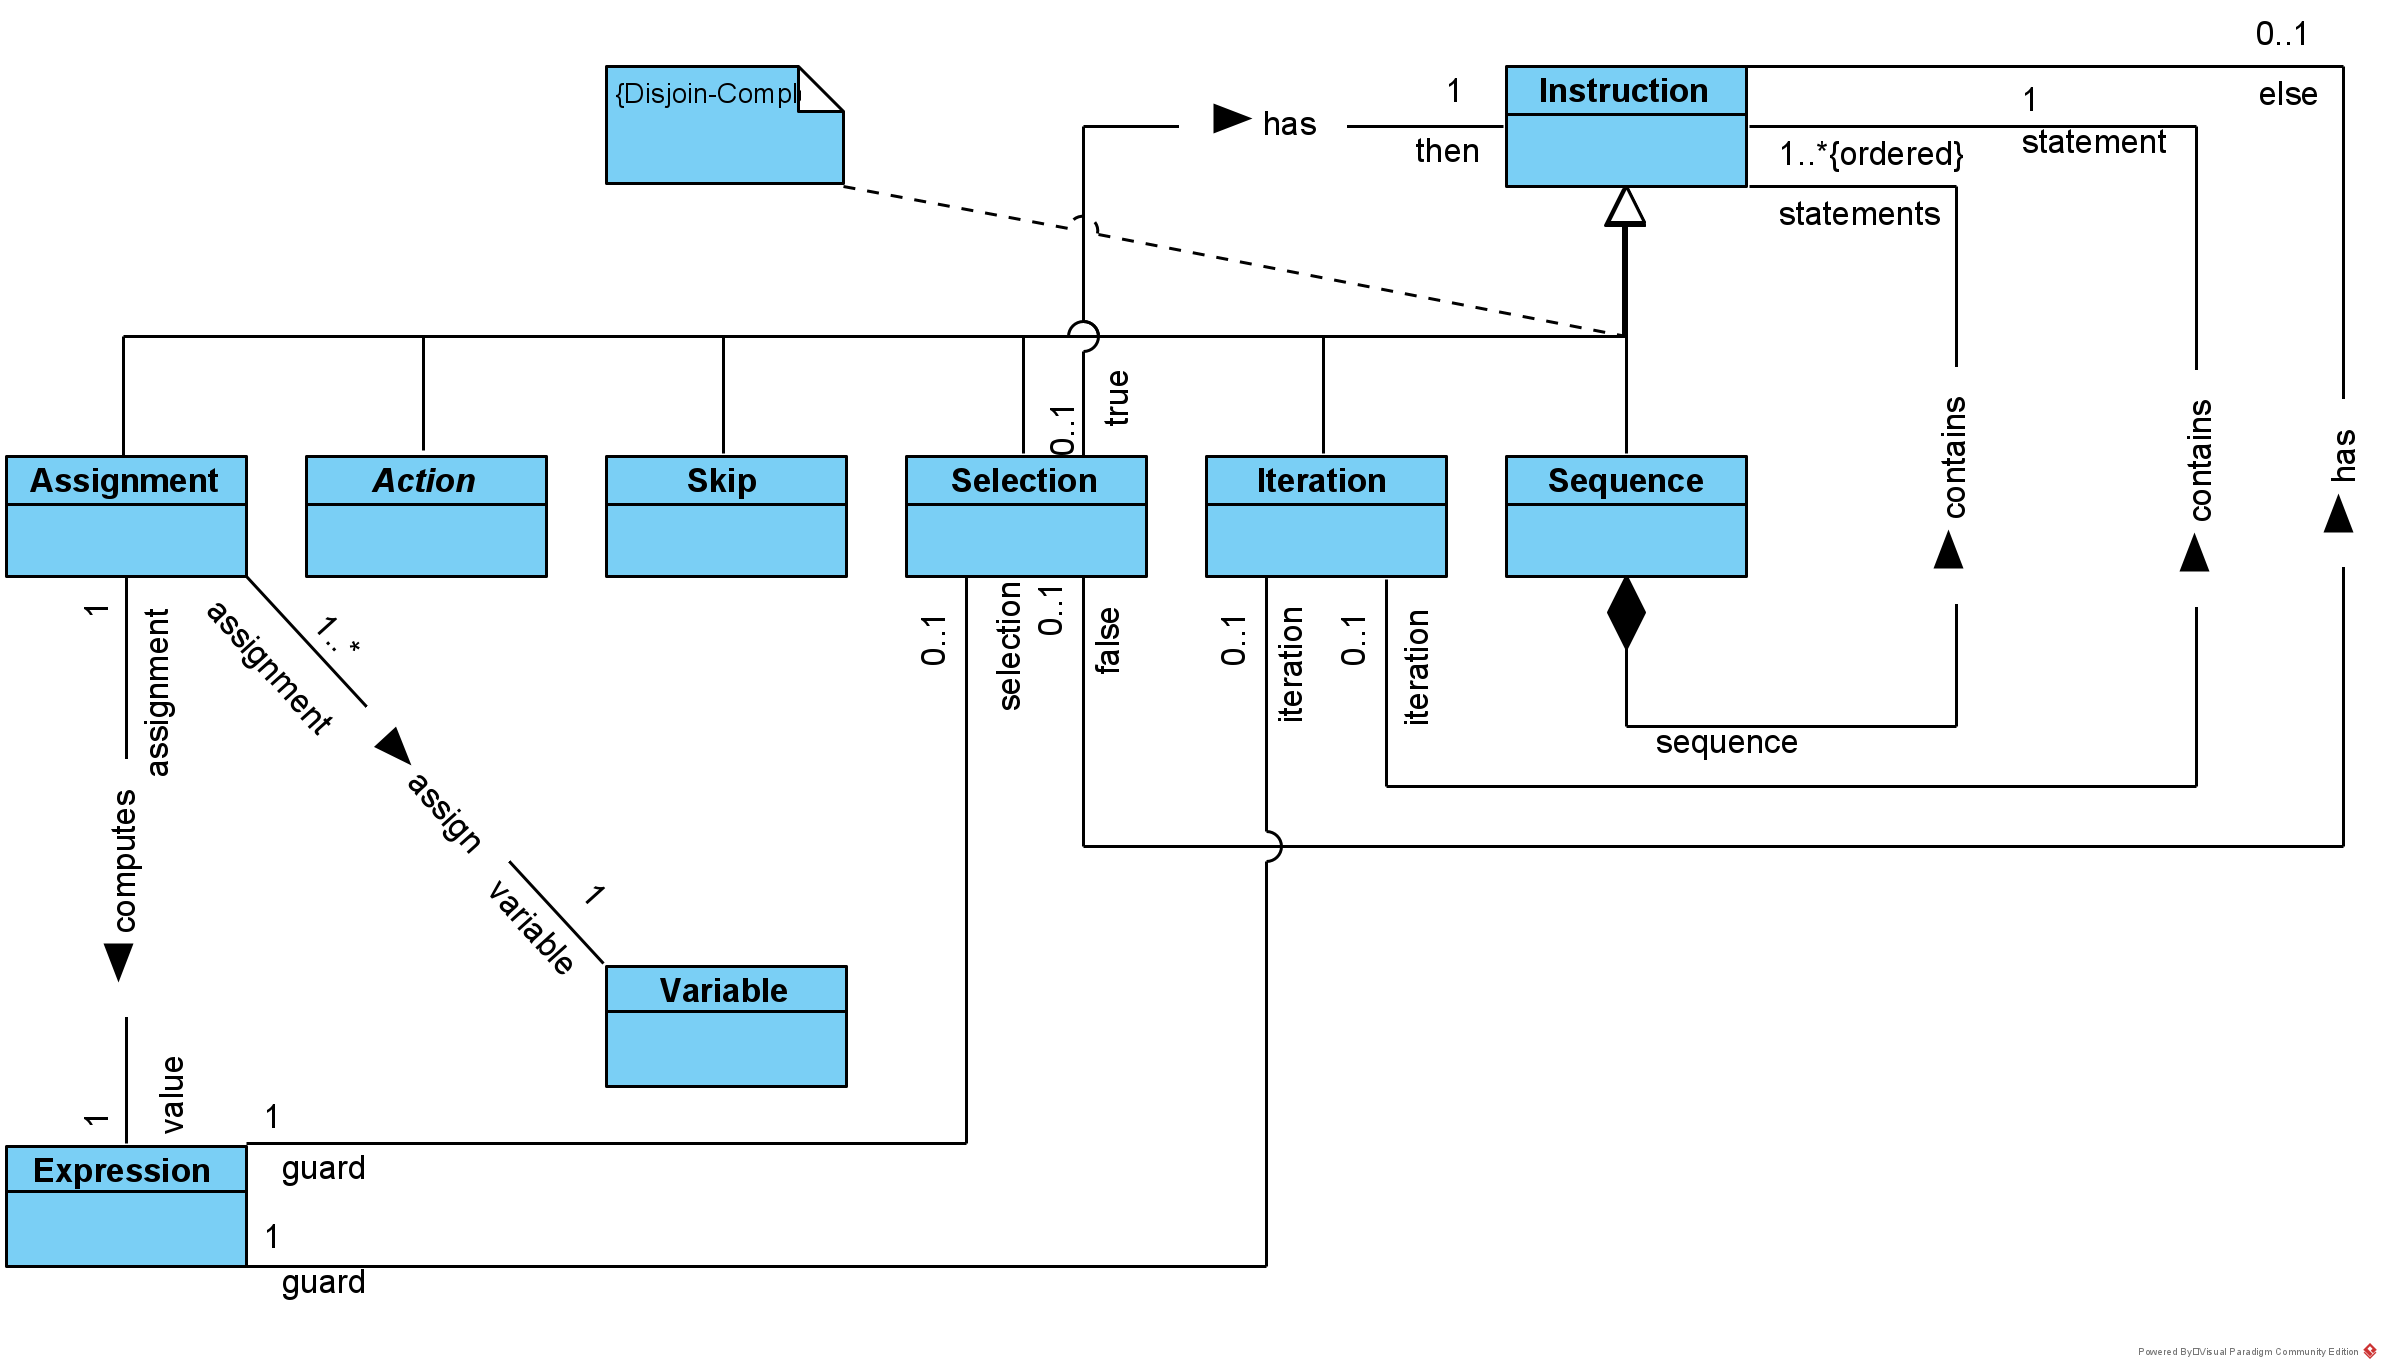
\includegraphics[width=\textwidth,height=\textheight,keepaspectratio]{Diagrams/DS-Instruction.png}

Séquences, itérations et sélections sont des instructions qui n'existent que pour permettre l'occurrence d'autres instructions. 
\begin{itemize}
    \item Les séquences forment le gros de ces instructions : 
    \begin{itemize}
        \item toute instruction forme à elle seule une séquence de 1 instruction.
        \item toute déclaration de module implique la déclaration d'une séquence d'instructions pour former son corps.
        \item tout réaction déploie l'action d'un personnage à travers une série d'instructions et de tests pour déterminer l'action immédiate à prendre. 
    \end{itemize}
    Une séquence d'instruction est, comme son nom l'indique, une suite ordonnée d'instructions. Prises dans le désordre, elles perdraient tout leur sens.
    \item Les itérations sont des instructions qui appellent la même instruction (qui peut être une séquence ou une sélection) encore et encore, sur base d'une expression de contrôle (la garde).
    \item Les instructions de sélection (ou branchement) permettent de choisir entre une (séquence d')instruction(s) gauche(s) et une (séquence d')instruction(s) droite(s), en fonction du résultat du test de la garde. Nous avons choisi de modéliser cette instruction par deux associations distinctes : cela nous permet de mettre en avant la contrainte d'avoir exactement deux branches distinctes, dont l'une est facultative.
\end{itemize}

On retrouve donc, comme pour les expressions, un principe fort de récursion dans les instructions.

Pour terminer la récursion, nous avons trois instructions terminales :
\begin{itemize}
    \item \textit{Je pause} (\textit{skip}), qui vise à signifier l'absence d'action.
    \item \textit{Je réfléchis} (\textit{Assignment}), qui vise à préserver en mémoire le résultat d'une procédure de calcul.
    \item \textit{J'agis} (\textit{Action}), qui vise à réaliser le comportement (sur base d'un arbre d'instructions et des éléments qui auront été mémorisés).
\end{itemize}

\section{Contraintes d'unicité}

\lstset{
	tabsize=4,
	rulecolor=,
	language=[Decorative]OCL,
    emph={self,@pre,@post},emphstyle={\color{dark-green}},
    basicstyle=\footnotesize\ttfamily,
    upquote=true,
    aboveskip={1.5\baselineskip},
    columns=fixed,
    showstringspaces=false,
    extendedchars=true,
    breaklines=true,
    prebreak = \raisebox{0ex}[0ex][0ex]{\ensuremath{\hookleftarrow}},
    frame=single,
    showtabs=false,
    showspaces=false,
    showstringspaces=false,
    stringstyle=\color{pred},
    keywords={oclType, selectByType, post, pre, def, inv, context, let,one,indexOf},
    deletendkeywords={name},
    deletekeywords=[3]{Enumeration},
    keywordstyle=\color[rgb]{0,0,1}\slshape\bfseries,
    commentstyle=\color[rgb]{0.133,0.545,0.133},
    stringstyle=\color[rgb]{0.627,0.126,0.941},
}

\textbf{Question 4.14.}\label{Question 4.14.}\newline

\nopagebreak 

Spécifier les contraintes d'unicité suivantes :

\begin{itemize}
    \item Les modules ont un nom unique au sein d'une même stratégie;
    \begin{lstlisting}
context Strategy inv uniqueModules : 
    self.declarations->selectByType(Module)
        ->forAll(m1,m2|m1<>m2 implies m1.name <> m2.name)
    \end{lstlisting}
    Nous vérifions ici que toutes les déclarations de module d'une même stratégie utilisent un nom différent.

    \item Les variables globales ont un nom unique au sein d'une même stratégie;
    \begin{lstlisting}
context Strategy inv uniqueGlobalVars : 
    self.declarations->selectByType(Variable)
        ->forAll(v1,v2|v1<>v2 implies v1.name<>v2.name)
    \end{lstlisting}
    
    De la même manière, nous vérifions ici que, pour une même stratégie, toutes les déclarations qui concernent des variables utilisent un nom différent.

    \item Les variables locales au sein d'un module possèdent un nom unique;
    \begin{lstlisting}
context Module inv uniqueLocalVars : 
    self.parameters->forAll(v1,v2|v1<>v2 implies v1.name<>v2.name)
    \end{lstlisting}
    
    Nous regroupons ici les variables locales déclarées par le module, qui doivent être toutes nommées différemment.
    \begin{tcolorbox}
        Nous ne vérifions pas ici si les variables locales sont des redéfinitions de variables globales.
    \end{tcolorbox}

    \item Les noms des paramètres d'un module sont tous différents;
    \begin{lstlisting}
context Module inv uniqueParameters : 
    self.parameters->forAll(p1,p2|p1<>p2 implies p1.name<>p2.name)
    \end{lstlisting}
    
    Nous vérifions ici que les paramètres sont tous nommés différemment. Nous ne vérifions par contre pas si les paramètres et les variables déclarés au sein d'un même module ne sont pas en conflit pour un même nom. 
    \begin{tcolorbox}
        \item Pour ce faire, il aurait fallu joindre les deux collections de type \textit{bag} puis comparer à nouveau les valeurs entre elles :
        \begin{lstlisting}
context Module inv uniqueVariables : 
    self.parameters->union(self.variables)->forAll(e1,e2|e1<>e2 implies e1.name<>e2.name)
        \end{lstlisting}
    \end{tcolorbox}

    \item Les noms des types déclarés sont globalement uniques (en particulier, on ne peut pas nommer une énumération et un tableau de manière identique);
    \begin{lstlisting}
context DataType inv uniqueTypeName : 
    Datatype.AllInstances()->forAll(dt1,dt2|dt1<>dt2 implies dt1.name<>dt2.name)
    \end{lstlisting}
    Pour toutes les instances de type de données existantes simultanément (indépendamment de leur localisation), il n'existe aucun autre type qui porte le même nom.
    
    \begin{tcolorbox}
        Nous posons ici le choix fort d'utiliser la méthode \textit{AllInstances} pour s'assurer qu'il ne puisse jamais y avoir de redéfinition d'un type à aucun moment dans le code. Cette démarche nous a semblé acceptable dans la mesure où le nombre de types déclarés devrait rester dans un ordre de grandeur simple.
    \end{tcolorbox}
    
\end{itemize}

\section{Contraintes de règles}

\textbf{Question 4.15.}\label{Question 4.15.}\newline

\nopagebreak 

\textit{Spécifier une contrainte OCL permettant de vérifier qu'une déclaration de type est bien formée :}

\nopagebreak

\begin{itemize}
    \item La liste des littéraux est unique au sein d'une énumération;
    \begin{lstlisting}
context Enumeration inv uniqueLiterals :
    self.literals->forAll(l1,l2|l1<>l2 implies l1.value<>l2.value)
    \end{lstlisting}
    
    \item \textit{liste des champs d'un enregistrement est non-vide ; }
    
    Ce point est déjà couvert par une contrainte de multiplicité sur l'association \textit{"[1]record has [1..*] fields"}.
    
    \item \textit{les noms des champs sont uniques au sein d'un même enregistrement ;}
    \begin{lstlisting}
context Record inv uniqueFields : 
    self.fields->forAll(f1,f2|f1<>f2 implies f1.name<>f2.name)
    \end{lstlisting}
    
    \item \textit{un tableau comporte au moins une dimension ;}
    
    Il n'est pas nécessaire de préciser cette contrainte en OCL : celle-ci est déjà présente dans la cardinalité de l'attribut multiple \textit{dimensions} du tableau : celui-ci doit être strictement supérieur ou égal à 1.
    
    
    \item \textit{Chaque dimension de tableau doit être strictement positive.}
    \begin{lstlisting}
context Array inv positiveDimension : 
    self.dimensions->forAll(dimension|dimension>0)
    \end{lstlisting}
    
\end{itemize}

\section{Programmation par contrat}

\subsection{Expression::type()}

\textbf{Question 4.16.}\label{Question 4.16.}\newline

\nopagebreak 

\textit{Supposons l'existence d'une opération} Expression :: type() : Type \textit{définie dans la classe} Expression\textit{. Spécifier le contrat sur le résultat produit par cette opération pour vérifier que le type retourné correspond :}\newline

Pour répondre à cette question, nous allons d'abord détailler les différents cas de figures de manière individuelle. Une contrainte OCL complète unifiant tous les cas sera ensuite proposée en fin de réponse.

\begin{itemize}
    \item \textit{au type du littéral (par exemple, le type de la valeur} true \textit{doit d'être} Boolean \textit{, celui de la chaîne} "123" \textit{doit d'être} String \textit{et celui de l'entier} 122 Integer\textit{, etc.) ;}
    \begin{lstlisting}
context PrimitiveLiteral::type(): DataType
    pre  nothing      : --none
    post primitiveType: result = self.type
    \end{lstlisting}
    \begin{itemize}
        \item \textbf{Précondition} : aucune précondition spécifique n'est à déclarer pour cette opération.
        \item \textbf{Postcondition} : Le résultat est le type primitif associé à ce litéral.
    \end{itemize}
    

    \item \textit{à l'opérateur unaire, à condition que sa sous-expression corresponde à ce type. Par exemple, les types de expressions unaires} -123 \textit{et} not isVisible \textit{doivent respectivement d'être} Integer \textit{(puisque} 12 \textit{est entier) et} Boolean \textit{(à condition que la variable} isVisible \textit{soit déclarée comme une variable booléenne) ;}
    \begin{lstlisting}
context UnaryOperator::type(): DataType
    pre nothing   : --none
    post unaryType: result = self.operand.type()
    \end{lstlisting}
    \begin{itemize}
        \item \textbf{Précondition} : aucune précondition spécifique n'est à déclarer pour cette opération.
        \item \textbf{Postcondition} : Le résultat est le type déduit depuis la sous-expression.
    \end{itemize}
    
    Nous prenons ici le parti de la récursivité : tant que l'expression contient une sous-expression, l'opération \textit{type()} continue de s'appeler, jusqu'à atteindre une expression litérale ou un symbole qui renvoie vers un type de données modélisé.

    \item l\textit{e type correspondant à l'opérateur binaire, à condition que les types des sous-expressions soient cohérentes. Par exemple,} 12 + total \textit{utilise un opérateur entier} + \textit{sur deux sous-expressions entières, mais} 12 + isVisible \textit{est incohérent ;}
    \begin{lstlisting}
context BinaryOperator::type(): DataType
    pre  isValidBinary: self.operands->forAll(e1,e2|e1.type=e2.type)
    post binaryType   : result = self.operands->first().type()
    \end{lstlisting}

    \begin{itemize}
        \item \textbf{Précondition} : les deux membres de l'expression binaire doivent être de même type.
        \item \textbf{Postcondition} : le résultat est le type de la première expression. 
    \end{itemize}
    
    Nous savons par précondition que les deux expressions sont de même type : l'une ou l'autre peut donc être choisie arbitrairement et renvoyer tout de même le bon résultat. Nous utilisons en outre à nouveau la récursion sur les types d'expression.

    \item \textit{le type de la sous-expression dans une expression parenthésée ;}
    \begin{lstlisting}
context Group::type(): DataType
    pre nothing  : --none
    post exprType: result = self.expression.type()
    \end{lstlisting}
    \begin{itemize}
        \item \textbf{Précondition} : aucune précondition spécifique n'est à déclarer pour cette opération.
        \item \textbf{Postcondition} : Le résultat doit être le type déduit de la sous-expression.
    \end{itemize}
    
    Une fois encore, nous nous appuyons sur la récursivité présente dans le super-type expression.

    \item \textit{le type de sa déclaration pour une expression d'accès à la valeur d'une variable (cf. exemples plus haut avec} isVisible{) ;}
    \begin{lstlisting}
context Symbol::type(): DataType
    pre  nothing   : --none
    post symbolType: result = self.variable.type
    \end{lstlisting}
    \begin{itemize}
        \item \textbf{Précondition} : aucune précondition spécifique n'est à déclarer pour cette opération.
        \item \textbf{Postcondition} : le résultat est le type déclaré de la variable.
    \end{itemize}
    
    Cette opération est permise grâce à la partition incomplète des sous-types de \textit{Symbol} : certains symboles ne sont en effet que des références vers des variables \textit{normales} et peuvent donc renvoyer que le type de cette variable. Pour les symboles à indices ou à champs, une méthode surchargée sera appliquée (cf. ci-dessous).

    \item \textit{le type de l'énumeration pour une expression d'un accès à un littéral d'énumération. Par exemple, `Direction.Up` doit renvoyer le type énumération `Direction` ;}
    \begin{lstlisting}
context EnumerationLiteral::type(): DataType
    pre  nothing : --none
    post enumType: result = self.enum
    \end{lstlisting}
    \begin{itemize}
        \item \textbf{Précondition} : aucune précondition spécifique n'est à déclarer pour cette opération.
        \item \textbf{Postcondition} : le type renvoyé sera l'énumération à laquelle appartient le litéral d'énumération.
    \end{itemize}

    \item \textit{le type de la déclaration du champ dans une expression d'accès à un champ. Par exemple,} origine.x \textit{doit retourner} Integer \textit{puisque le champ} x \textit{est déclaré comme tel ;}
    \begin{lstlisting}
context AttributedSymbol::type(): DataType
    pre  isValidField : self.variable->oclAsType(Record)->one(field=self.field)
    post symbolType   : result = self.field.type
    \end{lstlisting}
    \begin{itemize}
        \item \textbf{Précondition} : la variable passée en paramètre doit être un enregistrement contenant le champ demandé par le symbole d'attribut.
        \item \textbf{Postcondition} : le résultat renvoyé est le type du champ.
    \end{itemize}
    
    \item l\textit{e type du contenu du tableau pour une expression d'accès à un élément de tableau. Par exemple, à partir des exemples déclarés en section} Types \textit{, les expressions} visible[0,0] \textit{et} area[0] \textit{doivent respectivement retourner} Integer \textit{et} VisibleLine \textit{.}
    \begin{lstlisting}
context IndexedSymbol::type(): DataType
    pre  isContained: self.element.index->size() 
                        = self.variable->oclAsType(Array).dimensions->size() and
                      self.element.index
                          ->forAll(i|i>=0 and 
                                     i<self.variable->oclAsType(Array)
                                           .dimensions->at(indexOf(index)))
    post symbolType : result = self.variable.type
    \end{lstlisting}
    \begin{itemize}
        \item \textbf{Précondition} : l'indice/les indices de l'élément recherché par le symbole indicé doivent être compris dans les limites de dimension du tableau correspondant.
        \item \textbf{Postcondition} : Le type retourné est le type déclaré du tableau.
    \end{itemize}
    
    Il s'agit ici de s'assurer que l'élément recherché appartient bien au tableau demandé. On présuppose ici que l'élément est de même type que le tableau.
    
\end{itemize}

Une fois toutes ces fonctions spécifiées, il suffit au moment de la réception d'une expression d'interpréter son sous-type et d'appliquer l'opération surchargée qui lui correspond.

\begin{minipage}{\linewidth}
    \begin{lstlisting}
context Expression::type(): DataType
    pre  nothing    : --none
    post literalType:
         if self.oclIsTypeOf(Group) 
       then result = self->oclAsType(Group).type()
       else if self.oclIsTypeOf(UnaryOperator) 
          then result = self->oclAsType(UnaryOperator).type()
          else if self.oclIsTypeOf(BinaryOperator)
             then result = self->oclAsType(BinaryOperator).type()
             else if self.oclIsTypeOf(PrimitiveLiteral) 
                then result = self->oclAsType(PrimitiveLiteral).type()
                else if self.oclIsTypeOf(EnumerationLiteral)
                   then result = self->oclAsTypeOf(EnumerationLiteral).type()
                   else if self.oclIsTypeOf(AttributedSymbol)
                      then result = self->oclAsType(AttributedSymbol).type()
                      else if self.oclIsTypeOf(IndexedSymbol)
                         then result = self->oclAsType(IndexedSymbol).type()
                         else result = invalid
                         endif
                      endif
                   endif
                endif
             endif 
          endif
       endif
    \end{lstlisting}
\end{minipage}

\begin{itemize}
    \item \textbf{Précondition} : aucune précondition spécifique n'est nécessaire ici.
    \item \textbf{Postcondition} : le résultat correspond au résultat propre au sous-type correspondant.
\end{itemize}

\begin{tcolorbox}
    La norme UML précise qu'une opération peut être redéfinie par un sous-type :\newline
    
\textit{An Operation may be redefined in a specialization of the featuringClassifier. This redefinition may add new preconditions or postconditions, add new raisedExceptions, or otherwise refine the specification of the Operation.} \cite[p.~117]{uml251spec2017} 

Il s'agit ici en effet d'appliquer le principe de \textit{substitution de Liskov} \cite{liskov2000}.
\newline

    Nous n'avons malheureusement pas pu trouver d'exemple concret permettant d'illustrer cette redéfinition et de confirmer notre notation : il y a fort à parier que l'opération décrite ci-dessus soit redondante en raison du principe de substitution, voire jamais appelée (puisque Expression est abstraite).
\end{tcolorbox}

\subsection{Avatar::canCross(tile:Tile): Boolean}

\textbf{Question 4.17.}\label{Question 4.17.}\newline

\nopagebreak 

\textit{Supposons l'existence d'une opération} estTraversableGraceAuxItems(...) : Boolean\textit{, qui rend vrai si et seulement si, pour un personnage donné, une case passée en paramètre est traversable grâce aux items que le personnage possède sans l'intervention du joueur, c'est-à-dire que la case est sur une zone de feu, d'eau ou de glace et que le personnage possède respectivement des bottes pare-feu, un kit de plongée et des bottes à crampon.}
\begin{itemize}
    \item \textit{Quelle classe de votre Diagramme de Classe pourrait contenir cette opération ?}
    
        La classe la plus appropriée est celle de l'avatar : c'est lui dont on veut vérifier la capacité à traverser une tuile donnée, en fonction des objets qu'il possède dans son inventaire.

    \item \textit{Définir cette opération en précisant quel(s) serai(en)t ses paramètre(s), et quel serait le contrat OCL sur cette opération.}

    \begin{minipage}{\linewidth}
    \begin{lstlisting}
    context Avatar::canCross(tile:Tile): Boolean
        pre validTile   : tile->notEmpty()
        post isCrossable: result = 
            tile.obstacle->isEmpty()
        or (tile.obstacle.oclIsTypeOf(Area) and
                (tile.obstacle.type=AreaType::FIRE
            or  (tile.obstacle.type=AreaType::ICE and
                 self.items->select(i|i.oclIsTypeOf(Capaciter) and
                                      i.type=CapaciterType::ICEBOOT)->notEmpty())
            or  (tile.obstacle.type=AreaType::WATER and
                 self.items->select(i|i.oclIsTypeOf(Capaciter) and
                                      i.type=CapaciterType::DIVEMASK)->notEmpty())))
        or (tile.obstacle.oclIsTypeOf(Area) and
            self.items->select(i|i.oclIsTypeOf(Buff) and
                                 i.type=BuffType::CAPE)->notEmpty())
        or (self.items->select(i|i.oclIsTypeOf(Buff) and
                                 i.type=BuffType::CAPE and
                                 i.useLeft>0)->notEmpty())
        \end{lstlisting}
    \end{minipage}
    \begin{itemize}
        \item \textbf{Précondition} : la tuile doit être non-nulle.
        \item \textbf{Postcondition} : la tuile est traversable selon plusieurs cas de figure.
        \begin{itemize}
            \item La tuile ne contient aucun obstacle.
            \item La tuile contient une zone de feu et l'avatar peut la franchir sans condition. Le fait d'avoir des \textit{bottes de feu} ne lui permet que d'éviter de perdre des PV.
            \item La tuile contient une zone d'eau ou de glace et dans ce cas, l'avatar doit posséder l'objet-capaciteur correspondant.
            \item La tuile contient une zone et le personnage possède la cape de mage dans ses objets.
            \item La tuile contient n'importe quel obstacle et le personnage possède la cape de mage avec des points d'utilisation restants.
        \end{itemize}
    \end{itemize}
    
        Il s'agit ici de vérifier uniquement si la tuile concernée est traversable par le joueur : rien ne nécessite de vérifier si l'avatar du joueur est placé à côté ni même si la tuile fait partie du plateau de jeu sur lequel se trouve l'avatar.
        
        \begin{tcolorbox}
        Nous appliquons ici le \textit{principe de responsabilité unique} \cite{martin2003agile}.
        \end{tcolorbox}
        
        Nous ne vérifions pas non plus que la tuile ne contient pas d'ennemi, puisque ce n'est pas l'objet de la méthode et que cette contrainte est déjà exprimée sur le diagramme de classe par les cardinalités.
    
\end{itemize}

\subsection{Avatar::collect(): Void}

\textbf{Question 4.18.}\label{Question 4.18.}\newline

\nopagebreak 

\textit{Supposons l'existence d'une opération} ramasser(...) : Void \textit{dont l'effet est le suivant : si la case passée en paramètre contient un item ramassable, alors préciser le contexte (càd. sur quelle classe est défini l'opération) et la signature (càd. les paramètres) de l'opération ramasser et définir le contrat sur son résultat.}\newline

La classe à laquelle s'applique cette opération est bien entendu \textit{Avatar} : le contexte est défini par le personnage, puisque c'est lui qui bénéficie de l'opération de ramassage.

\begin{itemize}
\begin{minipage}{\linewidth}
    \item \textit{Si l'item est un bonus de défense ou d'attaque, le ratio correspondant du personnage se trouve modifié en multipliant l'ancienne valeur par la valeur du bonus ;}

\begin{minipage}{\linewidth}
    \begin{lstlisting}
context Avatar::collectBooster(booster:Booster): Void
    pre  itemPresent: booster->notEmpty()
    post apBooster  : 
          if booster.type=BoosterType::ATTACK
        then self.attackRatio = self.attackRatio@pre * booster.value
        else self.attackRatio = self.attackRatio@pre
        endif
    post dpBooster  : 
          if booster.type=BoosterType::DEFENSE
        then self.defenseRatio = self.defenseRatio@pre * booster.value
        else self.defenseRatio = self.defenseRatio@pre
       endif
    \end{lstlisting}
\end{minipage}

    \begin{itemize}
        \item \textbf{Précondition} : l'objet doit être non-nul.
        \item \textbf{Postcondition} : en fonction du type de Booster ramassé, le ratio d'attaque ou de défense de l'avatar est modifié proportionnellement à la valeur du booster.
    \end{itemize}
\end{minipage}

    \item \textit{Si l'item est un radar, il double la visibilité de la position de l'adversaire ;}
    
\begin{minipage}{\linewidth}
    \begin{lstlisting}
context Avatar::collectPointer(pointer:Pointer): Void
    def packedRadar : 
        Pointer = self.items->selectByType(Pointer)
                            ->select(i|i.oclAsType(Pointer).type=Pointer::RADAR)
                            ->first()
    def packedMap   : 
        Pointer = self.items->selectByType(Pointer)
                            ->select(i|i.oclAsType(Pointer).type=Pointer::MAP)
                            ->first()
    pre  itemPresent: pointer->notEmpty()
    post addRadar   : if pointer.type=Pointer::RADAR 
                    then if packedRadar->notEmpty()
                       then packedRadar.timeLeft = packedRadar.timeLeft@pre * 2
                       else self.items.append(pointer)
                      endif
                    else self.items=self.items@pre
                   endif
    post addMap     : if pointer.type=Pointer::MAP
                    then if packedMap->isEmpty()
                       then self.items.append(pointer)
                       else self.items = self.items@pre
                      endif
                    else self.items = self.items@pre
                   endif
    \end{lstlisting}
\end{minipage}
    \begin{itemize}
        \item \textbf{Précondition} : l'objet doit être non-nul.
        \item \textbf{Postcondition} : Si l'avatar possède déjà un radar dans son inventaire, sa durée restante est doublée, sinon le nouveau radar est ajouté à l'inventaire.
    \end{itemize}

    \item \textit{Si l'item est de la nourriture, de l'eau, des munitions, des bottes, des palmes, une cape ou une cotte de maille, l'item est simplement rajouté dans l'inventaire.}
\begin{minipage}{\linewidth}
    \begin{lstlisting}
context Avatar::collectConsumable(consumable:Consumable): Void
    pre  itemPresent: consumable->notEmpty()
    post isPacked: self.items.append(consumable)
    \end{lstlisting}
\end{minipage}
\begin{minipage}{\linewidth}
    \begin{lstlisting}
context Avatar::collectBuff(buff:Buff): Void
    pre  itemPresent: buff->notEmpty()
    post isPacked: self.items.append(buff)
    \end{lstlisting}
\end{minipage}
\begin{minipage}{\linewidth}
    \begin{lstlisting}
context Avatar::collectCapaciter(capaciter:Capaciter): Void
    pre  itemPresent: capaciter->notEmpty()
    post isPacked: self.items.append(capaciter)
    \end{lstlisting}
\end{minipage}
\begin{itemize}
    \item \textbf{Précondition} : l'objet doit être non-nul.
    \item \textbf{Postcondition} : l'objet est simplement ajouté à l'inventaire de l'avatar.
\end{itemize}

\end{itemize}

\begin{samepage}
Maintenant que nous avons défini les comportements propres à chaque type d'objet, nous pouvons établir le comportement général au ramassage d'objet :

\begin{minipage}{\linewidth}
    \begin{lstlisting}
context Avatar::collect(tile : Tile): Void
    def item       : Item = tile.item@pre
    pre isOnTile   : self.ground = tile
    post tileLooted: tile.item->isEmpty()
    post itemPacked:
            if item->notEmpty()
          then if item.oclIsTypeOf(Booster)
            then self.collectBooster(item->oclAsType(Booster))
            else if item.oclIsTypeOf(Consumable)
               then self.collectConsumable(item->oclAsType(Consumable))
               else if item.oclIsTypeOf(Pointer)
                  then self.collectPointer(item->oclAsType(Pointer))
                  else if item.oclIsTypeOf(Buff)
                     then self.collectBuff(item->oclAsType(Buff))
                     else if item.oclIsTypeOf(Capaciter)
                        then self.collectCapaciter(item->oclAsType(Capaciter))
                        else self = self@pre
                       endif
                   endif
                endif
             endif
          endif
    \end{lstlisting}
\end{minipage}
\end{samepage}

\begin{itemize}
    \item \textbf{Précondition} : l'avatar doit se trouver sur la tuile correspondante.
    \item \textbf{Postcondition} : si la tuile contient un objet, alors elle est \textit{pillée}, tandis que l'effet spécifique de l'objet est appliqué à l'avatar en fonction des règles énoncées ci-avant.
\end{itemize}

\subsection{Instruction::isValid()}

\textbf{Question 4.19.}\label{Question 4.19.}\newline

\nopagebreak 

\textit{Spécifier le contrat OCL sur une opération `Instruction::estValide(): Boolean` qui vérifie qu'une instruction est valide :}
\begin{itemize}
    \item \textit{L'instruction Skip est toujours valide ;}
        \begin{lstlisting}
context Skip::isValid(): Boolean
    pre  nothing: --none
    post isTrue : result = true
        \end{lstlisting}
        \begin{itemize}
            \item \textbf{Précondition} : aucune précondition n'est applicable pour cette opération.
            \item \textbf{Postcondition} : vrai dans tous les cas.
        \end{itemize}
    
    \item \textit{La garde d'une conditionnelle ou d'une itération doit être de type booléen ;}
        \begin{lstlisting}
context Selection::isValid(): Boolean
    pre  nothing     : --none
    post booleanGuard: result = self.guard.type().oclIsTypeOf(Boolean)
        \end{lstlisting}
        \begin{lstlisting}
context Iteration::isValid(): Boolean
    pre  nothing     : --none
    post booleanGuard: result = self.guard.type().oclIsTypeOf(Boolean)
        \end{lstlisting}
        \begin{itemize}
            \item \textbf{Précondition} : aucune précondition n'est applicable pour cette opération.
            \item \textbf{Postcondition} : vrai si la garde de l'instruction est une expression dont le type est \textit{Boolean}.\newline
            (cf. Question 4.16.).
        \end{itemize}
    
    \item \textit{La partie gauche et droite d'une affectation doivent être de même type.}
        \begin{lstlisting}
context Assignment::isValid(): Boolean
    pre  nothing : --none
    post sameType: result = self.variable.type = self.expression.type()
        \end{lstlisting}
        \begin{itemize}
            \item \textbf{Précondition} : aucune précondition n'est applicable pour cette opération.
            \item \textbf{Postcondition} : vrai si le type associé au symbole de destination correspond au type retourné par l'expression.\newline
            (cf. Question 4.16.)
        \end{itemize}
\end{itemize}

Maintenant que tous ces opérations sont décrites pour chaque sous-type, nous pouvons détailler l'opération générale.

\begin{minipage}{\linewidth}
        \begin{lstlisting}
context Instruction:IsValid(): Boolean
    pre  nothing : --none
    post sameType: 
            if self.oclIsTypeOf(Skip)
          then result = true
          else if self.oclIsTypeOf(Selection)
             then result = self->oclAsTypeOf(Selection).isValid()
             else if self.oclIsTypeOf(Iteration)
                then result = self->oclAsTypeOf(Iteration).isValid()
                else if self.oclIsTypeOf(Assignment)
                   then result = self.statements->forAll(s|s.isValid())
                   else if self.oclIsTypeOf(Assignment)
                      then result = self->oclAsTypeOf(Assignment).isValid()
                      else if self.oclIsTypeOf(Action)
                         then result = true
                         else return invalid
                        endif
                     endif
                  endif
               endif
            endif
         endif
        \end{lstlisting}
\end{minipage}

\begin{tcolorbox}
    A nouveau, nous utilisons le principe de redéfinition des opérations autorisé par la spécification UML \cite{uml251spec2017}, avec la réserve sur la formulation de l'opération au niveau du super type.
\end{tcolorbox}

\section{Questions de priorités}

\textbf{Question 4.20.}\label{Question 4.20.}\newline

\nopagebreak 

\textit{Spécifier une contrainte OCL vérifiant la cohérence des règles d'une stratégie par rapport à son objectif :}
\begin{itemize}
    \item \textit{Toutes les règles d'un même objectif (à court ou long terme) ont des priorités différentes pour assurer leur déclenchement déterministe.}
        \begin{lstlisting}
context Rule inv hasPriority : 
    self.priority->notEmpty()
    \end{lstlisting}
    \begin{lstlisting}
context Objective inv uniquePriorities : 
    self.rules.priorities->forAll(p1,p2|p1<>p2 
                                        implies p1.priority<>p2.priority)
        \end{lstlisting}
        On établit ici deux invariants
        \begin{itemize}
            \item Un invariant sur \textit{Rule} qui statue que toute directive a nécessairement une priorité.
            \item Un invariant sur \textit{Objective} qui s'assure que toutes les directive afférentes ont une priorité différente.
        \end{itemize}
        
    \item \textit{Une réaction de règle ne contient qu'une seule action `seDéplacer`.}
        \begin{lstlisting}
context Reaction inv uniqueMovement : 
    self.sequence->closure(statements)->forAll(statement|statement.oclIsKindOf(Action)) and 
    self.sequence->closure(statements)->selectByType(Move).size()=1
        \end{lstlisting}
        Une réaction ne peut être composée que d'une séquence d'instruction d'action, et celles-ci ne peuvent contenir qu'une seule action de mouvement.

    \item \textit{Seules les métarègles peuvent contenir l'action `changer`.}
        \begin{lstlisting}
context Rule inv changeOnlyMeta : 
    self.sequence->closure(statements)->exists(statement|statement.oclIsTypeOf(Change))
        implies self.meta=true
        \end{lstlisting}
        S'il existe une action de type changement parmi l'une des actions appartenant à une directive, alors cette dernière doit avoir le type \textit{"meta"}.
        \begin{tcolorbox}
            Il s'agit d'une implication: cela signifie qu'une règle méta n'a pas nécessairement d'action de type \textit{Change}.
        \end{tcolorbox}

\end{itemize}

\chapter{Diagrammes d'objet}

\section{Tile::containsGrail()}

\textbf{Question 4.21.}\label{Question 4.21.}\newline

\nopagebreak 

\textit{À partir de la situation définie en question 4.6, définir une stratégie constituée des visions suivantes:}
\begin{itemize}
    \item \textit{à long terme, se rendre vers le Graal;}
    \item \textit{à court terme, ramasser un maximum de nourriture.}
\end{itemize}
\textit{On ne définira pas les règles correspondantes, mais on déclarera en plus dans la stratégie un module} estCaseGraal(...) : Boolean\textit{ qui renvoie vrai si et seulement la case contient le Graal. On supposera une variable réservée} result\textit{ dont le type correspond au type de retour du module, et qui sera affectée du résultat.}

    \begin{lstlisting}
context Tile::containsGrail(): Boolean
    pre  nothing      : --none
    post containsGrail: result = tile.item->notEmpty() and 
                                 tile.item.oclIsTypeOf(Grail)
    \end{lstlisting}
    
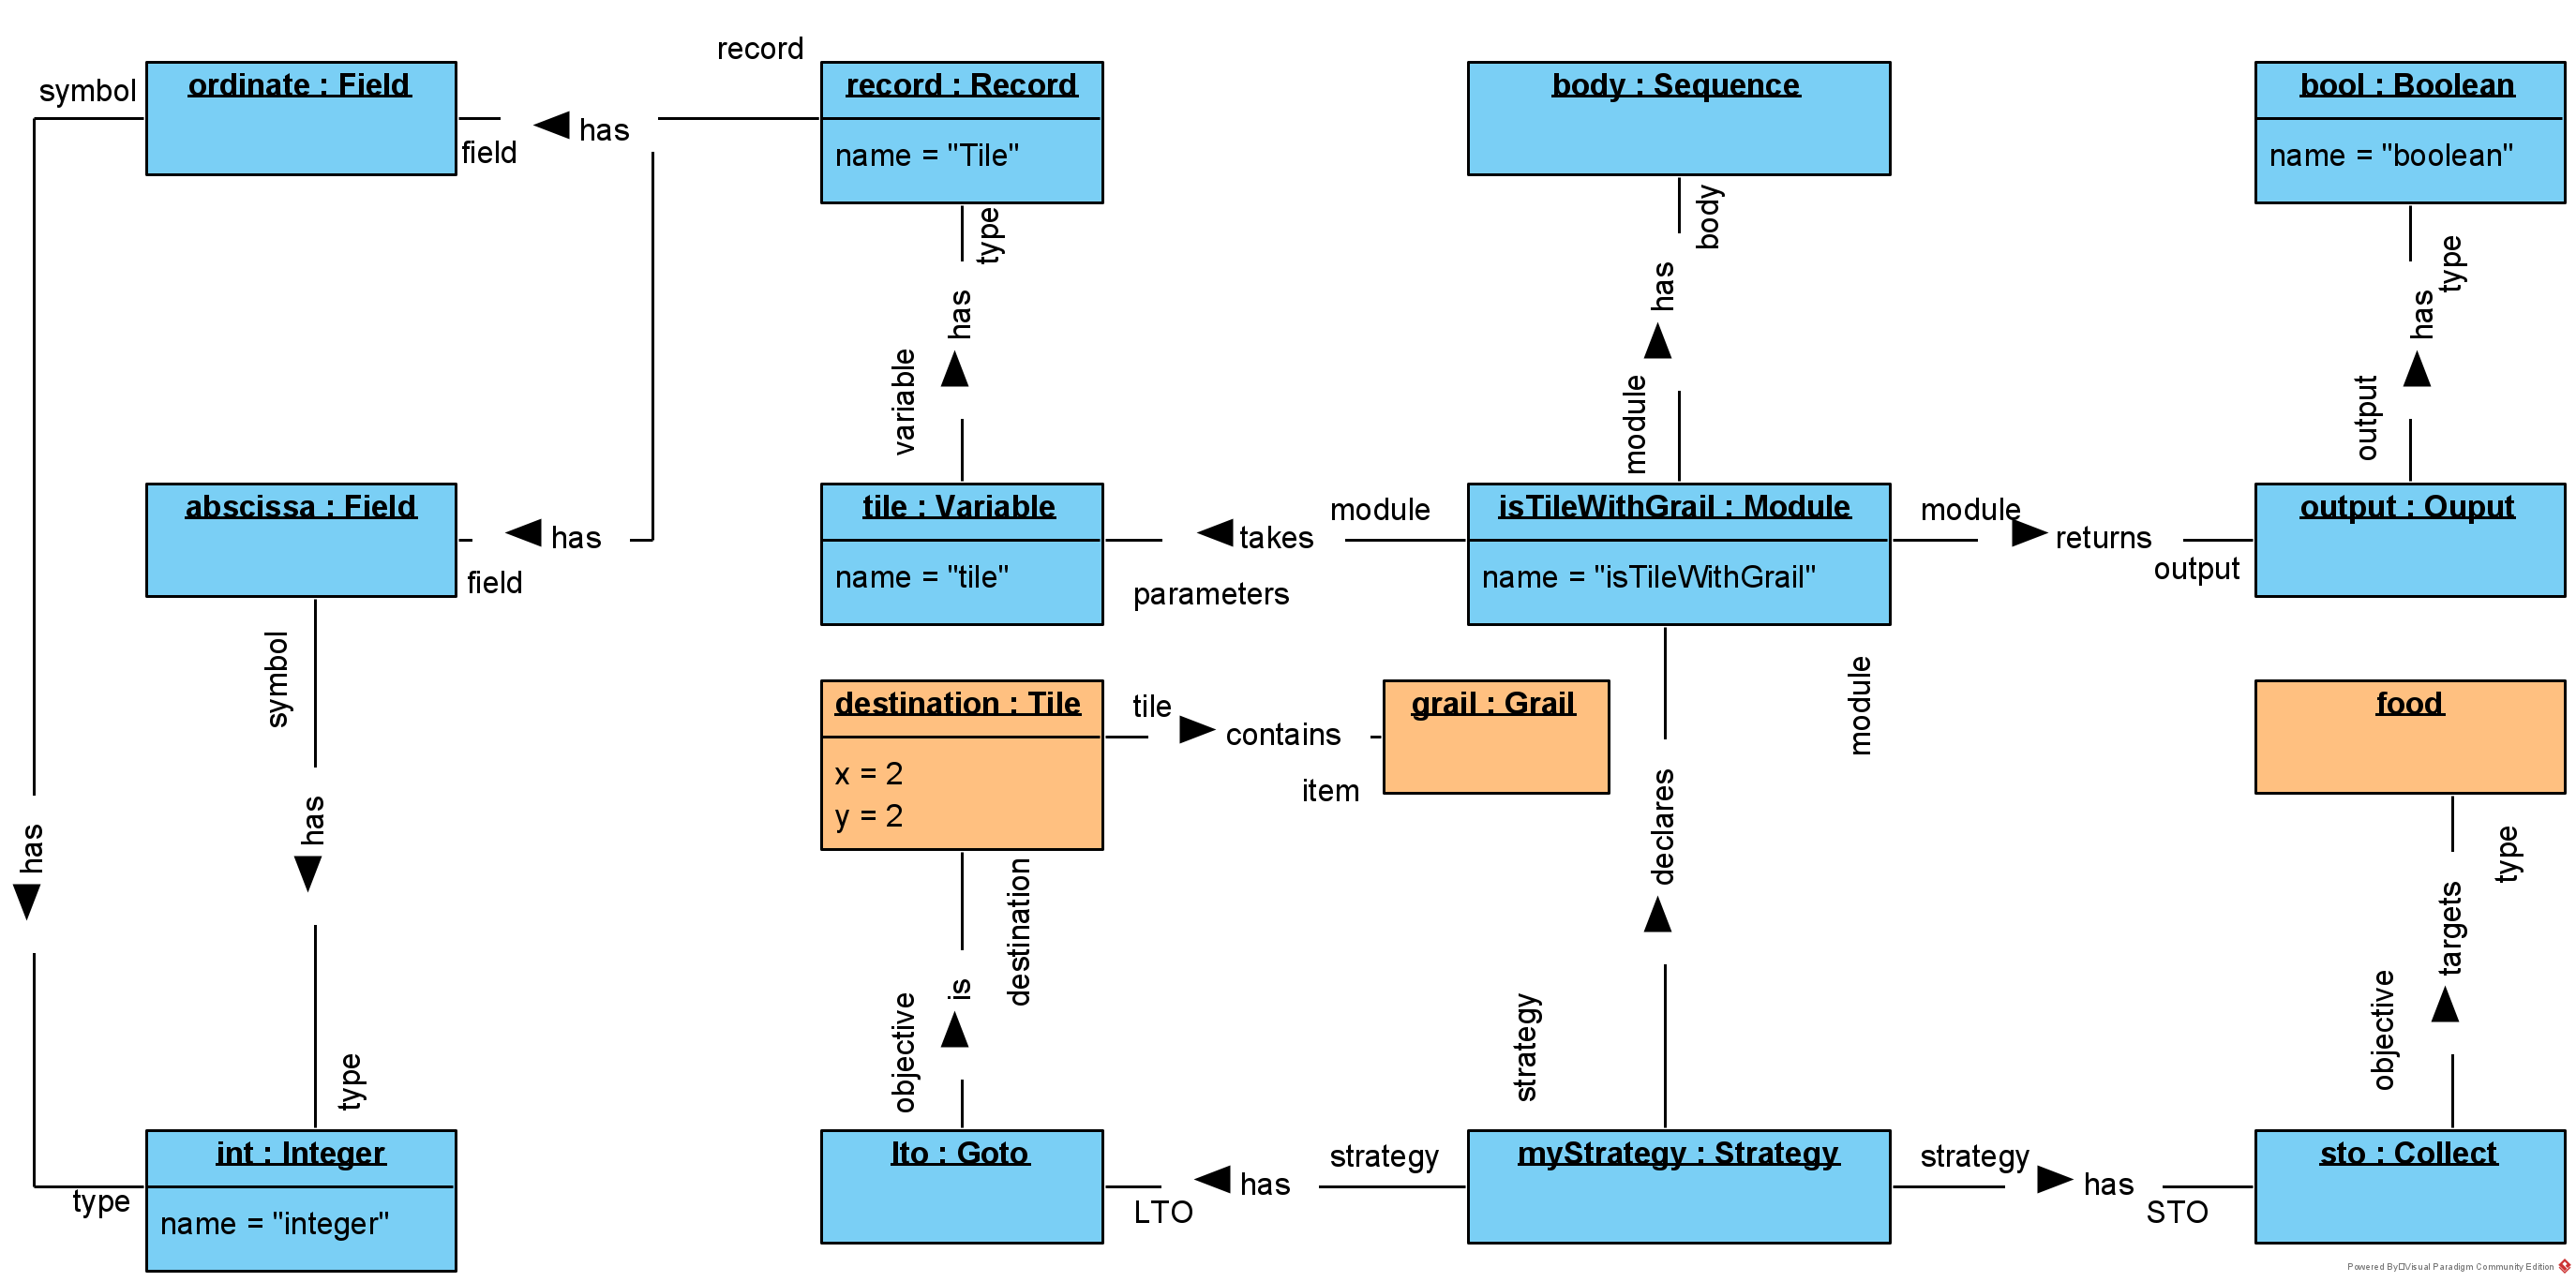
\includegraphics[width=\textwidth,height=\textheight,keepaspectratio]{Diagrams/OD-Strategy.png}\newline

La stratégie est composée de deux objectifs : 
\begin{itemize}
    \item Un objectif de long-terme de type GOTO (\textit{AllerVers}) - se rendre à une destination.
    \item Un objectif de court-terme de type COLLECT (\textit{CollecterMax}) - ramasser le plus d'objets possible sur le chemin.
\end{itemize}

\lstset{
	backgroundcolor=\color{lbcolor},
	tabsize=4,
	rulecolor=,
    emph={isTileWithGrail,x,y},emphstyle={\color{dark-green}},
    basicstyle=\footnotesize\ttfamily,
    upquote=true,
    aboveskip={1.5\baselineskip},
    columns=fixed,
    showstringspaces=false,
    extendedchars=true,
    breaklines=true,
    prebreak = \raisebox{0ex}[0ex][0ex]{\ensuremath{\hookleftarrow}},
    frame=single,
    showtabs=false,
    showspaces=false,
    showstringspaces=false,
    stringstyle=\color{pred},
    keywords={module, param,produces, begin,end, type, var},
    classoffset=1,
    keywordstyle={\color[rgb]{0,0,1}\bfseries},
    classoffset=0,
    commentstyle=\color[rgb]{0.133,0.545,0.133},
    stringstyle=\color[rgb]{0.627,0.126,0.941},
}

Pour réaliser ces objectifs, la stratégie a déclaré un module permettant de tester si une tuile contient le Graal.  Ce module accepte un paramètre en entrée (une tuile \textit{tile}), produit une sortie de type booléen, et est composé d'une séquence indéterminée d'instructions.
    \begin{lstlisting}
module isTileWithGrail
param tile : Tile
produces boolean
begin
    ...
end
    \end{lstlisting}

Le type tuile est un symbole de type \textit{Record} composé lui-même de deux champs (\textit{Field}) dont le type est \textit{Integer}. Ce sont ces champs qui nt la position de la tuile.
    \begin{lstlisting}
type Tile : record
    x : integer;
    y : integer;
endrecord
    \end{lstlisting}

\chapter{Maturité et modularité}

\textbf{Question 4.22}\label{Question 4.22.}\newline
\textit{Dans l'état actuel du jeu, une case ne peut pas superposer un item sur un obstacle. Pourtant, ce serait parfois utile de donner au joueur un gros bonus à condition qu'il puisse traverser une zone de feu.}

\begin{itemize}
    \item \textit{Comment proposeriez-vous de modifier votre diagramme de définition du monde pour intégrer cette possibilité ?}
    
            Dans le diagramme de base, un invariant spécifie qu'il ne peut y avoir soit qu'un obstacle soit qu'un objet sur une tuile. Il suffit de retirer cet invariant pour permettre à une tuile de contenir simultanément un obstacle et un objet.
          
    \item \textit{Quel impact cela a-t-il sur votre modélisation du langage de stratégie, et sur les contraintes OCL définies de part et d'autre ?}
        
    Puisque la contrainte était exprimée par un invariant, il n'y a pas de contrainte OCL à ré-écrire ou à supprimer ou de changement à apporter au DSL.
    
\end{itemize}

\newpage
\chapter{Conclusion}

La réalisation de ce laboratoire nous a permis de comprendre la difficulté qu'il peut y avoir à modéliser correctement un phénomène lorsqu'il est spécifié de manière informelle : nous avions commencé ce travail en construisant les objets au fur et à mesure de la spécification, sans analyse préparatoire. Ceci nous a conduit à de nombreuses erreurs et incompatibilités et a rendu nécessaire de revoir le modèle à de nombreuses reprises.\newline

Notre compréhension du sujet a réellement évolué à partir du moment où nous avons réalisé une liste exhaustive et précise de l'ensemble des spécifications ainsi qu'un glossaire. Cela nous a en effet permis de clarifier les concepts, de réduire les ambiguïtés et d'effectuer des recoupements. De cette analyse, nous avons pu dresser la liste des différentes classes nécessaires et commencer la réalisation des diagrammes.\newline

Nous nous sommes ensuite attaqué à la réalisation des associations et avons pu nous confronter à la seconde difficulté qu'entraîne un exercice de modélisation : la rapidité avec laquelle un certain modèle peut prendre forme et sembler complet vis-à-vis de notre sujet. Pour s'assurer que notre modèle est correct, il faut régulièrement le remettre à l'épreuve, que ce soit à la suite de changements dans d'autres sections du diagramme ou simplement pour s'assurer qu'il répond aux conditions énoncées. Nous avons ainsi dû revenir plusieurs fois sur une partie du modèle pour la reformuler entièrement, parce qu'un aspect manquait dans la conceptualisation (importance du \textit{rubber duck debug} \begin{tikzpicture}[scale=0.2]\duck[mask=teal,cape=teal]\end{tikzpicture}).\newline

En conclusion, nous retiendrons l'importance du systématisme et de la documentation dans la réussite d'une modélisation : découpe claire des concepts, choix des termes et harmonisation.

\newpage

\part{Annexes}
\chapter*{Spécifications}
\addcontentsline{toc}{chapter}{Spécifications}  
\renewcommand*{\theHsection}{chY.\the\value{section}}
\setcounter{chapter}{1}
\renewcommand{\thesection}{\arabic{section}}

\section{Description du jeu}

\subsection{Game}
Le \textbf{jeu} est la raison principal de ce laboratoire : il s'agit d'une construction complexe permettant à des êtres humains de se divertir en s'opposant de manière ludique.
    
\subsection{Series}
La \textbf{série} est le coeur même du jeu : c'est au cours de séries que les joueurs peuvent effectivement \textit{jouer} les uns avec les autres.
    \begin{itemize}
        \item Une série possède un identifiant unique..
        \item Une série est composée d'un ensemble de rencontres.
            \begin{itemize}
                \item Une série de rencontres comprend au moins une rencontre.
                \item Le nombre de rencontres au sein d'une série est impair.
                \item Les rencontres sont jouées en ordre successif.
                \item Une seule rencontre peut être jouée à la fois.
                \item Chaque rencontre ne peut être jouée qu'une seule fois.
            \end{itemize} 
        \item Une série est gagnée par le joueur qui a remporté le plus de rencontres durant la série. 
            \begin{tcolorbox}
                Il se peut que la série ne compte pas de gagnant.
            \end{tcolorbox}
        \item Une série peut se jouer selon deux modes :
            \begin{itemize}
                \item DUEL :        mode duel (2 joueurs uniquement)
                \item MULTIPLAYER : mode multi-joueurs (3+ joueurs)
            \end{itemize}
        \item Une série est jouée selon deux formules :
            \begin{itemize}
                \item REALTIME :   soit en formule temps-réel (également appelée \textit{interactive}).
                \item TURN-BASED : soit en formule tour-par-tour (également appelée \textit{éducative}).
            \end{itemize}
        \item En formule éducative, les joueurs ne jouent pas directement, mais choisissent des stratégies.
        \item Pour initier une nouvelle série, les joueurs humains doivent :
            \begin{itemize}
                \item Choisir le mode de jeu.
                \item Choisir la formule de jeu et la limite de temps.\newline
                      Selon le type d'adversaire, une rencontre peut ou ne peut pas être chronométrée.
                    \begin{itemize}
                        \item Contre un ordinateur : FREE est autorisé.
                        \item Contre un ou plusieurs joueurs humains : FREE est interdit.
                    \end{itemize}
                \item S'ils jouent contre un ordinateur, choisir un niveau de difficulté.
                \item Choisir le nombre de rencontres que comptera la série.
                \item Choisir l'avatar qui le représentera au cours de cette partie
            \end{itemize}
    \end{itemize}
    
\subsection{Match}
La \textbf{rencontre} est le composant d'une série au cours de laquelle les joueurs s'affrontent effectivement par le biais de leurs avatars.
    \begin{itemize}
        \item Un rencontre est identifié de manière unique.
        \item Toute rencontre se déroule sur un plateau propre.
        \item Une rencontre ne peut pas être rejouée.
        \item Un rencontre voit se rencontrer les avatars des joueurs.
    
        \item Un match peut être libre ou limité:
            \begin{itemize}
                \item FREE : sans limite
                \item TIMER/TURN : soit par chronomètre, soit par compte-tours, selon la formule de jeu choisie.
            \end{itemize}
    
        \item Selon le type d'adversaire, une rencontre peut ou ne peut pas être chronométrée.
            \begin{itemize}
                \item Contre un ordinateur : FREE est autorisé.
                \item Contre un ou plusieurs joueurs humains : FREE est interdit.
            \end{itemize}
        
        \item La limite d'une rencontre ainsi choisie s'exprime soit:
            \begin{itemize}
                \item en temps restant.
                \item en tours restants.
            \end{itemize}
    
        \item Une rencontre peut être remporté de deux manières :
            \begin{itemize}
                \item LAST-MAN-STANDING : seul un dernier avatar est encore en vie.
                \item FOUND-GRAIL : un avatar a trouvé le Graal.
            \end{itemize}
        \begin{tcolorbox}
            Une rencontre peut ne pas compter de vainqueur, si le temps restant est écoulé/le nombre de tours autorisés dépassés, ou si les deux derniers avatars meurent au même moment.
        \end{tcolorbox}
        
        \item Au cours d'une rencontre, les avatars suivent les directives de stratégies choisies pas les joueurs.
    \end{itemize}
    
\subsection{Player}
Le \textbf{joueur} est un acteur principal dans le jeu : c'est lui qui détermine et participe aux séries de rencontres, donne des instructions aux avatars et remportent les victoires.
    \begin{itemize}
        \item Un joueur possède un nom unique qui l'identifie parmi tous les joueurs.
        \item Un joueur est soit un être humain, soit un ordinateur.
        \item Un ordinateur a trois niveaux de difficulté possibles
            \begin{itemize}
                \item BEGINNER
                \item NORMAL
                \item EXPERT
            \end{itemize}
        \item Un joueur possède des apparences, dont au moins une apparence par défaut.
        \item Un joueur possède au moins un avatar et peut en avoir davantage.
        \item Un joueur participe à des séries pour jouer.    
        \item Un joueur possède un historique des séries et rencontres jouées et remportées, ainsi que des opposants dans ces parties.
        \item Au cours d'une rencontre, les joueurs voient :
            \begin{itemize}
                \item Le plateau de jeu, avec 
                    \begin{itemize}
                        \item Les limites du plateau.
                        \item Le brouillard de guerre.
                        \item La tuile sur laquelle leur avatar est positionné.
                        \item Un ensemble de tuiles du plateau dans un périmètre autour de l'avatar, défini par la ligne de mire de celui-ci
                        \item Leur avatar.
                    \end{itemize}
                \item Une barre de menu avec
                    \begin{itemize}
                        \item Les caractéristiques de cet avatar.
                        \item L'inventaire courant de cet avatar.
                    \end{itemize}
            \end{itemize}
    \end{itemize}
    
\subsection{Avatar}
L'\textbf{avatar} est le composant qui s'affronte effectivement sur les plateaux de jeu.
    \begin{itemize}
        \item Un avatar est possédé par un et un seul joueur.
        \item Un avatar possède un identifiant unique parmi les avatars d'un joueur.
        \item Un avatar porte une et une seule apparence (qui peut être changée).
        \item Un avatar se trouve au maximum sur une et une seule tuile.
        \item L'avatar possède un inventaire.
        \item Un avatar possède différentes caractéristiques : 
        \begin{itemize}
            \item Un potentiel de vie, exprimé en points.
            \item Des niveaux d'attaque et de défense, exprimés en ratios.
            \item Une portée de vue
        \end{itemize}
        \item Un avatar dont les points de vies sont à zéro meurt. Il perd la rencontre en cours et est retiré du plateau.
        \item Un avatar possède un inventaire rassemblant les objets collectés par l'avatar au cours des différentes rencontres.
        \item Un avatar peut utiliser différents objets pour s'aider au cours d'une rencontre.
        \item Un avatar est la cible des attaques des zombies à proximité.
        \item Un avatar suit les directives d'une stratégie en mode tour-par-tour.
        \item Un avatar est positionné sur 0 ou 1 tuile (suivant qu'il est utilisé dans une partie ou non).
        \item Un avatar possède des coordonnées absolues, correspondant à la tuile sur laquelle il se trouve.
    \end{itemize}
    
\begin{tcolorbox}
    La description du jeu ne précise pas explicitement ce qu'il se passe lorsqu'un avatar meure au cours d'une rencontre en milieu de série :
    \begin{itemize}
        \item Est-ce que le joueur doit choisir un remplaçant pour continuer la série ?
        \item Est-ce que le joueur perd immédiatement la série, sans jouer les rencontres restantes\:?
        \item Est-ce que l'avatar est \textit{ressuscité} avec des caractéristiques par défaut et un inventaire donné ?
    \end{itemize}
\end{tcolorbox}
    
\subsection{Skin}
L'\textbf{apparence} est une représentation graphique d'un avatar.
    \begin{itemize}
        \item Une apparence est soit libre, soit payant (\textit{premium}).
        \item Une apparence est disponible mais pas forcément encore acquise par un des joueurs.
        \item Une apparence peut être porté par n'importe quel avatar, pour autant que son joueur-propriétaire l'ait acheté préalablement.
        \item Il existe au moins une apparence non-payante.
    \end{itemize}

\subsection{Inventory}
L'\textbf{inventaire} représente un ensemble d'objets appartenant à un même avatar.
    \begin{itemize}
        \item Au cours des rencontres, les avatars accumulent des objets, qu'ils stockent dans leur inventaire.
        \item À la fin d'une rencontre et d'une série, certains objets sont conservés, d'autres sont défaussés.
        \item L'inventaire d'un avatar peut contenir
            \begin{itemize}
                \item Un stock de munitions/boissons.
                \item Des objets lui conférant de nouvelles aptitudes permanentes.
                \item Des objets à activer qui confèrent des aptitudes temporaires.
            \end{itemize}
    \end{itemize}

\subsection{Board}
Le \textbf{plateau} de jeu est l'endroit sur lequel s'affrontent les joueurs au cours d'une rencontre.
    \begin{itemize}
        \item Au cours de la rencontre, les avatars des joueurs se déplacent sur et interagissent avec les éléments du plateau.
        \item Un plateau est de dimension figée et carrée.
        \item Un plateau est découpé selon une grille bi-dimensionnelle.
        \item Un plateau est composé de tuiles, en nombre spécifié par ses dimensions.
        \item Les tuiles du plateau sont posées les unes à côtés des autres de manière ordonné et bidimensionnelle.
        \item Il n'existe pas de "trou" au sein d'un plateau.
        \item Un plateau est habité par des personnages qui sont soit les avatars des joueurs, soit des zombies contrôlés par l'ordinateur.
        \item Un plateau est toujours délimité par une rangée d'obstacles infranchissables sur son contour.
        \item Au début d'une rencontre, le plateau de jeu est entièrement révélé aux joueurs pour leur permettre d'établir une stratégie. Le plateau est ensuite recouvert d'un brouillard de guerre, permettant aux avatars de voir les tuiles dans un périmètre défini par leur ligne de mire.
    \end{itemize}
    
\subsection{Tile}
La \textbf{tuile} est le composant principal, atomique, du plateau de jeu.
\begin{itemize}
    \item Une tuile possède des coordonnées absolues qui renseignent sa position sur le plateau.
    \item Une tuile peut être positionnée à côté de 0 à 4 tuiles adjacentes, selon les quatre directions cardinales.
    \item Une tuile peut de manière facultative contenir différents éléments :
        \begin{itemize}
            \item Un personnage (avatar ou zombie).
            \item Un obstacle.
            \item Un objet.
        \end{itemize}
      \item Une tuile ne peut avoir au maximum qu'un seul personnage présent à la fois.
      \item Une tuile ne peut avoir au maximum qu'un seul obstacle présent à la fois.
      \item Une tuile ne peut avoir au maximum qu'un seul objet présent à la fois.
      \item Une tuile ne peut contenir simultanément un obstacle et un objet.
    \end{itemize}

\subsection{Zombie}
Le \textbf{zombie} est le personnage antagoniste aux avatars.
    \begin{itemize}
        \item Un zombie se trouve nécessairement sur une tuile sur un plateau donné.
        \item Un zombie erre dans le monde sans but, jusqu'à apercevoir un avatar.
        \item La distance à partir de laquelle un zombie aperçoit un avatar est fonction de son ratio d'attaque.
        \item Lorsqu'il aperçoit un avatar, le zombie se lance à sa poursuite : il essaye de s'en rapprocher, puis d'effectuer une attaque au corps-à-corps.
        \item Un zombie effectue une attaque au corps-à-corps lorsqu'il frappe une tuile adjacente dans la direction observée par le zombie.
        \item Un zombie n'attaque pas les autres zombies.
        \item Un zombie ne collecte pas les objets présents sur le plateau.
        \item Un zombie est présent sur une et une seule tuile.
        \item Un zombie a, comme les avatars, un certain nombre de caractéristiques.
        \begin{itemize}
            \item Un potentiel de vie, exprimé en points
            \item Un niveau d'attaque, exprimé sous forme de ratio.
            \begin{tcolorbox}
                Un zombie n'a pas de niveau de défense, contrairement aux avatars.
            \end{tcolorbox}
        \end{itemize}
        \item Un zombie dont le potentiel de vie est à zéro meurt et disparaît du plateau.
        \item Un zombie observe une direction parmi les directions cardinales.
        \item Un zombie adapte sa direction à la suite de chaque mouvement : elle prend la valeur de la direction du mouvement effectué.
      \end{itemize}
      
\subsection{Obstacle}
Les \textbf{obstacles} sont des éléments de décor qui opposent une résistance aux personnages.
\begin{itemize}
    \item Un obstacle se trouve nécessairement sur une tuile sur un plateau donné.
    \item Un obstacle est parfois franchissable, parfois destructible.
        \begin{itemize}
            \item Un obstacle est \textit{franchissable} si un avatar peut le franchir sous certaines conditions :
                \begin{itemize}
                    \item par la possession d'un objet spécifique.
                    \item au prix d'un nombre défini de points de vie.
                \end{itemize}
            \item Un obstacle est \textit{destructible} si un avatar peut le détruire au moyen d'une attaque directe ou indirecte.
                \begin{itemize}
                    \item Un obstacle qui est détruit disparaît de la case et du plateau de jeu.
                \end{itemize}
        \end{itemize}
        
    \item Les obstacles destructibles sont :
        \begin{itemize}
          \item THORN : les ronces
          \item BUSH :  les buissons
          \item TRUNK : les troncs d'arbre
          \item SKULL : les têtes de mort
        \end{itemize}
    \item Les obstacles indestructibles sont répartis en deux catégories :
        \begin{itemize}
            \item Les obstacles permanents.
                \begin{itemize}
                    \item WALL : mur
                    \item TREE : arbre
                    \item ROCK : menhir
                \end{itemize}
            \item Les obstacles de zone.
                \begin{itemize}
                    \item FIRE : zone de feu
                    \item ICE : zone de glace
                    \item WATER : zone d'eau
                \end{itemize}
        \end{itemize}
    \item Les conditions pour qu'un avatar puisse franchir un obstacle sont les suivantes :
        \begin{itemize}
            \item l'avatar possède la cape de mage et 
                \begin{itemize}
                    \item L'obstacle est une zone.
                    \item L'obstacle est un obstacle permanent ou destructible et la cape de mage possède des points d'utilisation restants.
                \end{itemize}
            \item L'obstacle est une \textit{zone de feu} et
                \begin{itemize}
                    \item l'avatar possède une cape de mage et/ou des bottes de feu.
                    \item autrement, l'avatar perd un nombre défini de points de vie.\newline Le nombre de points de vie perdu est fonction de la durée de séjour sur la zone de feu : 1 point par tour ou un nombre indéfini par minute.
                \end{itemize}
            
            \item L'obstacle est une \textit{zone d'eau} et l'avatar possède la cape de mage et/ou un kit de plongée
            \item L'obstacle est une \textit{zone de glace} et l'avatar possède la cape de mage et/ou des bottes à crampons.
        \end{itemize}
    \end{itemize}

\subsection{Item}
Les \textbf{objets} sont des éléments disséminés sur le plateau et pouvant être collectés par les joueurs pour leur conférer un avantage/une aptitude temporaire ou permanent.
\begin{itemize}
    \item Il existe plusieurs types d'objets :
        \begin{itemize}
            \item GRAIL : Graal.
            \item CONSUMABLE : consommables.
            \item BOOSTER : améliorants.
            \item CAPACITER : capaciteurs.
            \item BUFF : super-pouvoirs.
            \item POINTER : pointeurs.
        \end{itemize}

        \item Le \textit{Graal} est l'un des deux objectifs pour remporter une rencontre. 
            \begin{itemize}
                \item Il existe nécessairement un et un seul Graal sur le plateau.
                \item Il est activé automatiquement lorsque ramassé.
                \item Il ne rentre jamais dans l'inventaire.
            \end{itemize}
        
        \item Les \textit{consommables} permettent au joueur de récupérer des points de vie ou de lancer des projectiles.
        \begin{itemize}
            \item Les consommables sont de trois types :
                \begin{itemize}
                    \item FOOD : Nourriture
                    \item DRINK : Boisson
                    \item AMMO : Munitions
                \end{itemize}
            \item La nourriture et les boissons permettent de restaurer les points de vie de l'avatar.
            \item Les munitions permettent à l'avatar de lancer un projectile.
            \item Un consommable doit être activé pour réaliser son objet.
            \item Lorsqu'un consommable est activé, il est défaussé de l'inventaire.
            \item Les consommables non-utilisés sont permanents : ils restent dans l'inventaire de l'avatar après la fin de la rencontre et de la série.
        \end{itemize}

        \item Les \textit{améliorants} augmentent de manière permanente les caractéristiques de l'avatar qui les collecte.
            \begin{itemize}
                \item Les améliorants sont de deux types :
                    \begin{itemize}
                        \item ATTACK :  Boosteur d'attaque
                        \item DEFENSE : Boosteur de défense
                    \end{itemize}
                \item Les améliorants sont automatiquement activés lorsque ramassés par l'avatar.
                \item Les améliorants sont immédiatement défaussés après activation.
            \end{itemize}
            
        \item Les \textit{capaciteurs} confèrent une nouvelle aptitude permanente à l'avatar qui les collecte. 
            \begin{itemize}
                \item Les capaciteurs sont de trois types :
                    \begin{itemize}
                        \item FIREBOOT: bottes de feu.
                        \item ICEBOOT: bottes à crampons.
                        \item DIVEMASK: kit de plongée.
                    \end{itemize}
                \item Les bottes de feu permettent de franchir une zone de feu sans perdre de points de vie.
                \item Les bottes à crampons permettent de franchir une zone de glace.
                \item Le kit de plongée permet de franchir une zone d'eau.
                \item Les capaciteurs sont automatiquement activés lorsque ramassés par l'avatar.
                \item Les capaciteurs sont permanents : ils restent dans l'inventaire de l'avatar après la fin de la rencontre et de la série.
            \end{itemize}
            
        \item Les \textit{super-pouvoirs} donnent à l'avatar une capacité temporaire puissante.
            \begin{itemize}
                \item Les super-pouvoirs sont de deux types :
                    \begin{itemize}
                        \item ARMOR : cotte de mailles
                        \item CAPE : cape de mage
                    \end{itemize}
                \item La cotte de mailles rend l'avatar qui la porte insensibles aux attaques des autres avatars et zombies.
                \item La cape de mage permet à l'avatar qui la porte de traverser zones et obstacles sans dommages.
                \item La cape de mage ne permet de traverser des obstacles infranchissables que trois fois. Un compteur sous forme de points d'utilisation permet de mesurer combien d'utilisations restantes subsistent.
                \item Un super-pouvoir doit être activé pour réaliser son objet.
                \item Un super-pouvoir n'est actif que pour une durée limitée, exprimée en termes de temps ou nombre de tours restants, selon la formule de jeu retenue :
                \begin{itemize}
                    \item TURN-BASED: la durée correspond à [$\frac{1}{10}^e$ des points de vie de l'avatar].
                    \item REALTIME:   la durée correspond à $1$ minute.
                \end{itemize}
                \item Lorsqu'un super-pouvoir est activé, un compteur est enclenché et réduit progressivement la durée restante d'activité du super-pouvoir.
                \item Lorsqu'un super-pouvoir n'a plus de durée d'activité restante, il est défaussé de l'inventaire et l'avatar perd son pouvoir.
                \item Les super-pouvoirs non-utilisés sont permanents : ils restent dans l'inventaire de l'avatar après la fin de la rencontre et de la série.
            \end{itemize}
            
        \item Les \textit{pointeurs} aident l'avatar (et le joueur) à s'orienter vers le plateau, en indiquant la direction à vol d'oiseau vers le(s) autre(s) avatar(s) ou le Graal.
            \begin{itemize}
                \item Les pointeurs sont de deux types :
                    \begin{itemize}
                        \item MAP : carte.
                        \item RADAR : radar.
                    \end{itemize}
                \item La carte indique la direction à vol d'oiseau vers le Graal du plateau.
                \item La carte n'a pas de durée limitée.
                \item La carte est automatiquement activée lorsqu'elle est ramassée.
                \item La carte n'est pas permanente : elle est défaussée à la fin de la rencontre.
                \item Le radar indique la direction à vol d'oiseau vers le/les adversaire(s).
                \item Le radar doit être activé par l'avatar pour fonctionner.
                \item Le radar a une durée limitée, exprimée en terme de temps/tours restants.
                \item A chaque fois qu'un nouveau radar est ramassé, 
                    \begin{itemize}
                        \item si l'avatar ne possède pas encore de radar, il est simplement ajouté à l'inventaire.
                        \item si le joueur possède déjà un radar, celui-ci voit son temps restant d'utilisation doublé (qu'il soit actif ou non). Le nouveau radar est immédiatement défaussé.
                    \end{itemize}
                \item Les radars non-utilisés sont permanents : ils restent dans l'inventaire de l'avatar après la fin de la rencontre et de la série.
            \end{itemize}
        
        \item Un objet peut être ramassé par l'avatar présent sur la même tuile.
        \item Un objet ramassé disparaît du plateau et apparaît dans l'inventaire du joueur selon les conditions décrites ci-dessus.
    \end{itemize}

\section{Description des stratégies}

\subsection{Strategy}
Les \textbf{stragégies} sont des mécanismes de jeu automatique permettant au joueur de faire des rencontres en tour-par-tour.
    \begin{itemize}
        \item Une stratégie permet aux avatars d'effectuer des actions et des déplacements sans input direct des joueurs.
        \item Une stratégie est composée :
            \begin{itemize}
                \item d'objectifs ;
                \item de variables globales ;
                \item de modules.
            \end{itemize}
        \item Une stratégie comporte toujours deux objectifs :
            \begin{itemize}
                \item Un objectif de long-terme, à poursuivre en toutes circonstances.
                \item Un objectif de court-terme, à réaliser de manière opportuniste.
            \end{itemize}
        \item L'ordre de réalisation de ces objectifs est implicite :
        \begin{itemize}
            \item L'objectif de court-terme prime sur l'objectif de long-terme.
            \item Un objectif est réalisable tant qu'une de ses directives est activable.
            \item Un objectif néant est nécessairement précédé par l'autre objectif.
            \item Il ne peut pas y avoir deux objectifs néant au sein d'une stratégie.
        \end{itemize}
        \item Tous les modules au sein d'une stratégie sont nommés différemment.
        \item Toutes les variables globales au sein d'une stratégie sont nommées différemment.
    \end{itemize}

\subsection{Objective}
Les \textbf{objectifs} permettent de donner une direction et une liste d'actions possibles à des avatars pour remporter une rencontre.
    \begin{itemize}
        \item Un objectif est caractérisé par une cible :
            \begin{itemize}
                \item \textbf{Néant} (\textit{Random}) - déplacements aléatoires.
                \item \textbf{AllerVers} (\textit{Goto}) - déplacements en direction d'une tuile.
                \item \textbf{Contourner} (\textit{Avoid}) - déplacement en direction d'une tuile avec contournement.
                \item \textbf{Éviter} (\textit{Evade}) - déplacement d'éloignement d'un personnage ou d'une tuile.
                \item \textbf{CollecterMax} (\textit{Collect}) - priorisation du ramassage d'un certain type d'objet.
                \item \textbf{Combattre} (\textit{Attack}) - attaque de personnages avoisinants.
            \end{itemize}
        \item Les objectifs \textit{Néant} et \textit{Combattre} n'acceptent aucun paramètre.
        \item L'objectif \textit{AllerVers} prend en paramètre une tuile de destination.
        \item L'objectif \textit{Contourner} prend en paramètre une tuile de destination, ainsi qu'un ensemble de consignes d'évitements constituées d'un couple 
            \begin{itemize}
                \item élément à éviter et 
                \item direction à emprunter pour l'évitement.
            \end{itemize}
        \item L'objectif \textit{Éviter} prend en paramètre un personnage ou une tuile dont s'éloigner.
        \item L'objectif \textit{CollecterMax} prend en paramètre un type d'objet à rechercher et ramasser.
        \item Un objectif peut uniquement être changé au moyen d'une action Changer.
        \item Un objectif définit un ensemble de directives.
        \item Un objectif a nécessairement une directive par défaut. La priorité de cette directive a la valeur zéro.
        \item Lorsque plusieurs directives sont activées simultanément, seule celle dont la valeur de priorité est la plus proche de 0 est appliquée.
        \item Les priorités des directives d'un objectif sont toutes différentes.
        \item La directive par défaut n'a pas de pré-requis d'exécution.
    \end{itemize}
    
\subsection{Rule}
Les \textbf{directives} décrivent les actions à entreprendre pour la réalisation d'un objectif et les conditions dans lesquelles elles s'appliquent.
\begin{itemize}
    \item Il existe deux catégories de directives :
        \begin{itemize}
            \item les directives normales.
            \item les méta-directives.
        \end{itemize}
    \item Une directive est composée de trois éléments
        \begin{itemize}
            \item une priorité explicite (\textit{priority}.
            \item un déclencheur (\textit{trigger})
            \item une réaction (\textit{reaction})
        \end{itemize}
    \item La priorité indique le niveau de préséance d'une directive parmi les directives d'un objectif. 
        \begin{itemize}
            \item La priorité est un entier positif.
            \item Le niveau de priorité d'une directive est inversement proportionnel à sa valeur.
            \item La règle par défaut d'un objectif a la priorité zéro.
        \end{itemize}
    \item Le déclencheur est une expression booléenne qui, si elle est évaluée à vraie, signifie que la directive peut être appliquée.
    \item La réaction est un ensemble d'instructions élémentaires et de paramètres permettant la réalisation de la directive.
    \begin{itemize}
    \item Une réaction est composée de :
        \begin{itemize}
            \item des variables ;
            \item une séquence d'instructions.
        \end{itemize}
        \item Dans la séquence d'instructions, il peut y avoir plusieurs actions.
        \item Dans la séquence d'instructions, il ne peut y avoir qu'une seul action de type \textit{mouvement}.
        \item Seule une méta-directive peut inclure une action de type \textit{Changer}.
    \end{itemize}
\end{itemize}

\subsection{Action}
Les \textbf{actions} décrivent les interactions qu'un joueur peut entretenir avec le jeu et son avatar.
\begin{itemize}
    \item Il existe différent catégories d'action :
    \begin{itemize}
        \item \textbf{Mouvement} : action permettant au joueur de déplacer son personnage.
        \item \textbf{Activité} : action permettant au joueur d'interagir avec l'environnement direct du personnage.
        \item \textbf{Méta} : action permettant au joueur d'influer sur le comportement de son personnage.
    \end{itemize}
    \item L'action de mouvement est \textit{SeDéplacer} et consiste à modifier l'emplacement du personnage vers une tuile adjacente (en vérifiant les conditions de franchissement).
    \item Les actions de type \textit{activité} sont de cinq types :
    \begin{itemize}
        \item \textbf{Frapper} (\textit{slash})
        \item \textbf{Tirer} (\textit{fire})
        \item \textbf{Revêtir} (\textit{wear})
        \item \textbf{UtiliserItem} (\textit{use})
        \item \textbf{ConsulterRadar} (\textit{read})
    \end{itemize}
    \item L'action de frapper consiste 
\end{itemize}

\subsection{Module}
Les \textbf{modules} sont les éléments déclaratifs de la programmation et renseignent sur les calculs pouvant être réalisés et leur conditions d'exécution.
\begin{itemize}
    \item Un module est composé
        \begin{itemize}
            \item de variables locales ;
            \item de paramètres optionnels en entrée ;
            \item d'un retour facultatif ;
            \item d'un corps.
        \end{itemize}
    \item Un module possède un nom.
    \item Un module peut utiliser les variables globales de la stratégie à laquelle il appartient.
    \item Toutes les paramètres au sein d'un module sont nommées différemment.
    \item Toutes les variables au sein d'un module sont nommées différemment.
    \item Une variable locale ne peut avoir le même nom qu'une variable globale définie par la stratégie à laquelle le module appartient.
\end{itemize}

\subsection{Types}
Les \textbf{types} sont les éléments informatifs de la programmation et renseignent sur le format des données manipulées.
\begin{itemize}
    \item Il existe des types \textit{"finis"}, prédéfinis et figés.
    \item Il existe des types \textit{"extensibles"}, qui peuvent être ajoutés selon les besoins.
    \item Il existe différentes natures, ou formats : 
        \begin{itemize}
            \item Les types primitifs
            \item Les énumérations
            \item Les tableaux
            \item Les enregistrements
        \end{itemize}
    
    \item Les types \textit{primitifs} sont au nombre de 4 : string, integer, float, boolean.
    
    \item Les \textit{énumérations} établissent un ensemble fini de valeurs auto-expressives.
        \begin{itemize}
            \item Une énumération établit au moins une valeur.
            \item Les valeurs établies par une énumération porte un nom.
            \item Tous les noms de valeur d'une énumération doivent être différents.
        \end{itemize}
        
    \item Les \textit{tableaux} sont des séquences de valeurs, de longueur finie et organisées de manière multi-dimensionnelle.
        \begin{itemize}
            \item Un tableau possède un type (qui peut être un autre tableau).
            \item Un tableau définit une séquence de valeurs.
            \item Toutes les valeurs d'un tableau ont le même type.
            \item Un tableau possède au moins une dimension.
            \item La dimension d'un tableau doit être strictement positive.
        \end{itemize}
        
    \item Les \textit{enregistrements} sont des ensembles non-ordonnés et finis de valeurs de type variable.
        \begin{itemize}
            \item Un enregistrement déclare un ensemble de champs avec un certain type et un nom.
            \item Un enregistrement doit avoir au moins un champ.
            \item Les champs d'un enregistrement peuvent être de différents types.
            \item Les champs déclarés au sein un enregistrement possèdent un nom unique entre eux.
        \end{itemize}
    \item Les types possèdent un nom unique permettant de les identifier.
\end{itemize}


\subsection{Expression}
Les \textbf{expressions} sont l'élément de représentation textuelle des données dans le système.
\begin{itemize}
    \item Un expression peut être de six types :
        \begin{itemize}
            \item \textbf{Littéral} - un objet auto-exprimé.
            \item \textbf{Symbole} - un élément de la mémoire pouvant être assigné (LHS) ou récupéré (RHS).
            \item \textbf{Unaire} - Un opérateur unaire lié à un expression.
            \item \textbf{Binaire} - Un opérateur binaire lié à deux expressions.
            \item \textbf{Parenthésée} - Un groupe d'expressions
            \item \textbf{Appel de module} - un appel à un module prenant (ou non) des paramètres et produisant (ou non) un retour.
        \end{itemize}
    \item Un \textit{littéral} est une expression comprenant uniquement un élément auto-suffisant, c'est-à-dire un élément de type primitif ou une énumération.
    \item Un \textit{symbole} est une expression référençant un objet en mémoire pouvant être plus ou moins complexe.
    \item Une expression \textit{unaire} est une expression composée d'un opérateur unaire et d'un opérande. Cet opérande est lui-même une expression.
    \item Une expression \textit{binaire} est une expression composée d'un opérateur binaire et de deux opérandes : un à gauche et un à droite. Ces opérandes sont eux-mêmes des expressions.
    \item Une expression \textit{parenthésée} est une expression contenant une sous-expression entre deux marqueurs.
\end{itemize}

\subsection{Instruction}
Les \textbf{instructions} sont l'élément effectif de programmation qui permet de manipuler effectivement les données.
\begin{itemize}
    \item Une instruction peut être de cinq différents types :
        \begin{itemize}
            \item \textbf{Saut} (\textit{Skip}) - une instruction sans effet.
            \item \textbf{Conditionnelle} (\textit{Selection}) - une instruction de branchement, composée d'une garde et de 1 ou 2 branches (\textit{if...then...else...}).
            \item \textbf{Itération} (\textit{Iteration}) - une instruction de répétition, composée d'une garde de sortie et d'un corps d'instruction.
            \item \textbf{Séquence} (\textit{sequence}) - une instruction composée d'une suite d'instructions.
            \item \textbf{Affectation} (\textit{Assignment}) - une instruction composée d'une partie gauche et d'une partie droite et consistant à assigner la valeur de la partie droite dans la partie gauche.
            \item \textbf{Action} (\textit{Action}) - une instruction réalisant une action.
        \end{itemize}
    \item Elle permet
        \begin{itemize}
            \item de manipuler les données et
            \item d'effectuer des opérations : mouvements, interactions.
        \end{itemize}
\end{itemize}

\printglossary[nonumberlist, title={Glossaire}]

\nocite{ocl24}
\printbibliography[heading=bibintoc,title={Bibliographie}]

\end{document}
